\documentclass[12pt,twoside]{article}
%
%Packages----------------------------------------------------------
%\usepackage{german}  %  Alte Rechtschreibung
% \usepackage{ngerman} %  Neue Rechtschreibung
%\usepackage{showkeys}
\usepackage{amssymb}
\usepackage{caption}
%\usepackage{umlaute}
\usepackage[latin1]{inputenc}
\usepackage{defjs1}
\usepackage{psfig}
\usepackage{psfrag}
\usepackage{latexsym}
%\usepackage[draft]{graphicx}
% \usepackage{makeidx}     % allows index generation
\usepackage{graphicx}
\usepackage{multicol}    % used for the two-column index
\usepackage{psfrag}
\usepackage[usenames]{color}
%\usepackage[xdvi]{color}
\usepackage{ifthen}
\usepackage{fancyhdr}
\usepackage[T1]{fontenc}
\usepackage{epsfig}
\usepackage{bbm}




\usepackage[all]{xy}
\usepackage[usenames]{color}
\usepackage{epsfig}
\usepackage{rotating}
\usepackage{color}
\usepackage{colortbl}
\usepackage{slashbox}
%\usepackage{here} % \begin{figure}[H]  \includegraphicx{DATEINAME} \end{figure}
%                  Durch [H] wird erreicht, dass die Graphik nicht verschoben
%                  wird, sondern so wie im Quelltext platziert wird. Dazu benötigt 
%                  man noch das Package „here“.

\usepackage{alltt}  % Quellcodes per 'input' einlesen
%                     \begin{alltt}\input{quellcode}\end{alltt}
\usepackage{multirow}  % Mehrere Zeilen in tabular/array zusammenfassen



\def\sprl{\mbox{\boldmath $\Bigl[\hspace{-0.08cm}\mid$}}
\def\sprr{\mbox{\boldmath $\mid\hspace{-0.08cm}\Bigr]$}}

%-----------------------------------------------------------------------
%   BOLD FACE MATH ITALIC UNDERLINE:  MATRICES
%-----------------------------------------------------------------------
%
\newcommand{\matbA}{\underline{\bf A}}
\newcommand{\matbB}{\underline{\bf B}}
\newcommand{\matbC}{\underline{\bf C}}
\newcommand{\matbD}{\underline{\bf D}}
\newcommand{\matbE}{\underline{\bf E}}
\newcommand{\matbF}{\underline{\bf F}}
\newcommand{\matbG}{\underline{\bf G}}
\newcommand{\matbH}{\underline{\bf H}}
\newcommand{\matbI}{\underline{\bf I}}
\newcommand{\matbJ}{\underline{\bf J}}
\newcommand{\matbK}{\underline{\bf K}}
\newcommand{\matbL}{\underline{\bf L}}
\newcommand{\matbM}{\underline{\bf M}}
\newcommand{\matbN}{\underline{\bf N}}
\newcommand{\matbO}{\underline{\bf O}}
\newcommand{\matbP}{\underline{\bf P}}
\newcommand{\matbQ}{\underline{\bf Q}}
\newcommand{\matbR}{\underline{\bf R}}
\newcommand{\matbS}{\underline{\bf S}}
\newcommand{\matbT}{\underline{\bf T}}
\newcommand{\matbU}{\underline{\bf U}}
\newcommand{\matbV}{\underline{\bf V}}
\newcommand{\matbW}{\underline{\bf W}}
\newcommand{\matbX}{\underline{\bf X}}
\newcommand{\matbY}{\underline{\bf Y}}
\newcommand{\matbZ}{\underline{\bf Z}}
%
\newcommand{\matba}{\underline{\bf a}}
\newcommand{\matbb}{\underline{\bf b}}
\newcommand{\matbbb}{\underline{\bf b}}
\newcommand{\matbc}{\underline{\bf c}}
\newcommand{\matbd}{\underline{\bf d}}
\newcommand{\matbe}{\underline{\bf e}}
\newcommand{\matbbf}{\underline{\bf f}}
\newcommand{\matbff}{\underline{\bf f}}
\newcommand{\matbg}{\underline{\bf g}}
\newcommand{\matbh}{\underline{\bf h}}
\newcommand{\matbi}{\underline{\bf i}}
\newcommand{\matbj}{\underline{\bf j}}
\newcommand{\matbk}{\underline{\bf k}}
\newcommand{\matbl}{\underline{\bf l}}
\newcommand{\matbm}{\underline{\bf m}}
\newcommand{\matbn}{\underline{\bf n}}
\newcommand{\matbo}{\underline{\bf o}}
\newcommand{\matbp}{\underline{\bf p}}
\newcommand{\matbq}{\underline{\bf q}}
\newcommand{\matbr}{\underline{\bf r}}
\newcommand{\matbs}{\underline{\bf s}}
\newcommand{\matbt}{\underline{\bf t}}
\newcommand{\matbu}{\underline{\bf u}}
\newcommand{\matbv}{\underline{\bf v}}
\newcommand{\matbw}{\underline{\bf w}}
\newcommand{\matbx}{\underline{\bf x}}
\newcommand{\matby}{\underline{\bf y}}
\newcommand{\matbz}{\underline{\bf z}}

\newcommand{\matbnull}{\underline{\bf 0}}
\newcommand{\matbeins}{\underline{\bf 1}}
%
%-----------------------------------------------------------------------
%   Special Operators                           
%-----------------------------------------------------------------------
% some relevant fourth-order tensors
\newcommand{\IB}{\underline{\mathbb{B}}} % FEM B-Matrix mit Unterstrich
\newcommand{\IBB}{\mathbb{B}}            % FEM B-Matrix ohne Unterstrich
%\newcommand{\IN}{\underline{\mathbb{N}}} % FEM B-Matrix mit Unterstrich
%\newcommand{\INN}{\mathbb{N}}            % FEM N-Matrix ohne Unterstrich
\newcommand{\IT}{\mathbb{T}}
\newcommand{\IW}{\mathbb{W}}
\newcommand{\ISy}{\mathbb{S}}
%\newcommand{\IT}{{\rm T\kern-.45em T}} 
%\newcommand{\IW}{{\rm W\kern-.95em W}} 
%\newcommand{\ISy}{{\rm S\kern-0.415em S}} 
%
\def\sym{{\rm sym}}          %sym
\def\bone{{\bf 1}}           %bold 1
\def\bzero{{\bf 0}}          %bold 0
%
%\newcommand{\IH}{{\rm I\kern-.25em H}}           % H
%\newcommand{\II}{{\rm I\kern-.18em I}}           % 4th order identitytensor
%\newcommand{\IP}{{\rm I\kern-.18em P}}           % 4th order projectiontensor
\def\IR{{\rm I\kern-.25em R}}
%\def\IN{{\rm I\kern-.25em N}}                    % oben neu definiert
%
%\newcommand{\IA}{{\rm\kern.22em                  %fourth order tensor A
%    \vrule width.02em
%        height0.5ex depth 0ex
%    \kern-.24em A}}
%\newcommand{\IC}{{\rm\kern.24em                  %fourth order tensor C
%   \vrule width.02em height1.4ex depth-.05ex
%   \kern-.26em C}}
%\newcommand{\ID}{{\rm\kern.24em                  %fourth order tensor D (mak)
%   \vrule width.02em height1.6ex depth-.05ex
%   \kern-.30em D}}
%\newcommand{\IS}{{\rm\kern.24em                  %fourth order Eshelby tensor
%   \vrule width.02em height1.4ex depth-.05ex
%   \kern-.26em S}}
%















%Seitenlayout-------------------------------------------------------
\sloppy
\oddsidemargin   0.30cm            % linker Rand ungerade Seiten
\evensidemargin  0.30cm            % linker Rand gerade Seiten (twoside)
\topmargin       0.15cm            % OK Blatt - OK Kopfzeile
\topmargin      -1.35cm            % OK Blatt - OK Kopfzeile bei PS
\headheight      0.15cm            % H�e der Kopfzeile
\headsep         0.70cm            % UK Kopfzeile - OK Rumpf
\topskip         0.60cm            % OK Rumpf - UK Textzeile
\textheight     24.50cm            % Texth�e
\textwidth      16.00cm            % Textbreite
\footskip        1.00cm            % Uk Rumpf - UK Fu�eile
\fboxsep.3cm                       % Rahmenaufweitung 0.3cm
\setlength{\parindent}{0.0cm}      % Einzug 1. Zeile eines Absatzes
\setlength{\parskip}{1.ex}         % Abstand zweier Abs"atze
\setcounter{secnumdepth}{4}        % Tiefe der section Nummern
%Headings-----------------------------------------------------------
\setlength{\headheight}{16pt}
\pagestyle{fancy}
\renewcommand{\MakeUppercase}[1]{#1}    % Kopfzeilen nicht in gross
\fancyhead{Finite Element Method: Foundations, SS08, J. Schr\"oder, D. Balzani}  % Kopfzeile
\fancyhead[re] {\thepage}
\fancyhead[ro] {\thepage}
\fancyhead[ce] {\slshape}
\fancyhead[co] {\slshape}
\fancyfoot{}                            % Fusszeile
%%\fancyfoot[c]{\sffamily\small Version vom \today}
\fancypagestyle{plain}{%
  \fancyhead{}%
  \fancyfoot[c]{\sffamily\thepage}%
  \renewcommand{\headrulewidth}{0pt}%
}
\makeatletter                           % Leere Fuellseiten
\def\cleardoublepage{\clearpage\if@twoside \ifodd\c@page\else
  \hbox{}
  \vspace*{\fill}
  \thispagestyle{empty}
  \newpage
  \if@twocolumn\hbox{}\newpage\fi\fi\fi}
\makeatother
%\renewcommand{\chaptermark}[1]{\markboth {\chaptername\ \thechapter.\ #1}{}}
%\renewcommand{\sectionmark}[1]{\markright{\thesection\ #1}}
%
%Vorgaben Einbinden von Gleitobjektion-----------------------------
\setcounter{topnumber}{10}
\setcounter{bottomnumber}{10}
\setcounter{totalnumber}{10}
\renewcommand{\topfraction}{1.}
\renewcommand{\bottomfraction}{1.}
\renewcommand{\textfraction}{0.}
%-------------------------------------------------------------------
%\definecolor{mygrey}{gray}{0.75}
%-------------------------------------------------------------------
\renewcommand{\dir}{}
\newcommand{\setdir}[1]{\renewcommand{\dir}{#1}}
\newcommand{\load}[1]{\setdir{#1}%-------------------------------------------------------------------------
\sect{Classification of partial differential equations of 
second order}
\label{Section21}
%-------------------------------------------------------------------------
In this chapter some foundations and definitions are 
repeated in the context of partial differential equations 
with view to mechanical engineering problems. 
In the sequel we classify partial differential 
equations of second order and present prototypes of the 
particular classes. 

The linear partial differential equation in the two 
variables $\bx := (x_1 , x_2)^T$ and the unknown function 
$u (\bx )$ is given by 
%
\begin{equation}
  A(\bx) u,_{11} + 2 B(\bx) u,_{12} + C(\bx) u,_{22} + \dots
  = F(\bx) 
\label{eq:allgdgl}
\end{equation}
%
for all $\bx$ in the considered domain ${\cal B}$. 
Herein, we have used the abbreviations 
%
\begin{eqnarray}
  u,_{1} :=  \pp{u}{x_1} \, ; \quad u,_{11}  :=  \pppp{u}{x_1}{x_1} \, ; 
  \quad u,_{12} := \pppp{u}{x_1}{x_2} 
  \, ; \qquad \dots 
\end{eqnarray}
%
The type of partial differential equation depends on the 
sign of the discriminant 
%
\begin{equation}
\delta := AC-B^2
\label{eq:ac-b^2}
\end{equation}
%
in the considered domain. 
We distinguish between the following four cases: 
%
\begin{eqnarray}
\left. 
\begin{array}{l}
1. \; \delta < 0 : \textnormal{hyperbolic DE} \\
2. \; \delta = 0 : \textnormal{parabolic DE} \\
3. \; \delta > 0 : \textnormal{elliptic DE} \\
4. \; \delta \; \textnormal{modifies its sign: mixed type} \\
\end{array}
\right\} \, . 
\end{eqnarray}
%
The sign of the discriminant is invariant to any 
transformations of the independent variables. 
Hence, the type of the differential equation is an 
invariant with respect to the independent variables. 

In case of the classification of partial differential 
equations with more than two independent variables we 
consider the description 
%
\begin{equation}
\sum_{i,k} a_{ik} \pppp{u( \bx )}{x_i}{x_k} + \dots = 0
\label{eq:pdiff}
\end{equation}
%
with the symmetric real matrix $\bA = (a_{ik})$. 
If the coefficients $a_{ik}$ are no functions of the 
$\bx$, we refer to the differential equation as linear 
differential equation of second order with constant 
coefficients. 
By the use of a linear transformation, Equation 
(\ref{eq:pdiff}) can be reformulated by 
%
\begin{equation}
\sum_{i} \kappa_i \ppp{u (\bx )}{x_i^2}+ \dots = 0 \, ,
\end{equation}
%
in such a way that all coefficients $\kappa_i$ take the 
values $+1, -1$ or $0$. 

Depending on the signs we consider the following cases:
\begin{eqnarray}
\left. 
\begin{array}{ll}
1. & \textnormal{The DE is hyperbolic, if all coefficients 
          $\kappa_i$ differ from zero} \\
   & \textnormal{and one $\kappa_i$ has a converse sign
          with respect to the others.} \\
2. & \textnormal{The DE is parabolic, if one of the coefficients
          $\kappa_i$ vanishes} \\
   & \textnormal{and the others differ from zero and have the 
         same sign.} \\ 
3. & \textnormal{The DE is elliptic, if all coefficients 
         differ from zero} \\
   & \textnormal{and have the same sign.} \\
4. & \textnormal{An equation is called parabolic, 
         hyperbolic or elliptic, if it} \\
   & \textnormal{exhibits the corresponding characteristics 
         for all points of the domain.}
\end{array}
\right\}
\end{eqnarray}










{\bf Prototype of a hyperbolic differential equation: 
wave equation}

The motion of a string ${\cal B}$ with ${\cal B} \in [0,l]$, 
with given (zero) displacements at both ends, is described 
by 
%
\begin{eqnarray}
\left. 
\begin{array}{lrl}
\mbox{PDE}: & \dfrac{1}{c^2} u,_{tt} - u,_{11} = 0 & x \in {\cal B}
\, , t \ge 0 \\ [1.1ex]
\mbox{Boundary conditions:}   & u(0,t) = u(l,t) =  0 & t \ge 0 \\
\mbox{Initial state:}         & u(x,0) = u_0 (x) & x \in {\cal B} \\
\mbox{Initial velocity} & u,_t (x,0) = v_0 (x) & x \in {\cal B}
\end{array}
\right\}
\end{eqnarray}
%
Herein, the parameter $c>0$ characterizes the velocity 
of wave propagation. 
We consider the tranformed partial differential equation 
%
\begin{equation}
c^2 u,_{11} - u,_{tt} = 0
\end{equation}
%
and identify the values of the coefficients 
$A=c^2$, $B=0$ and $C=-1$. 
The discriminant 
%
\begin{eqnarray}
\delta=-c^2 < 0 \, ,
\end{eqnarray}
%
shows that the wave equation is hyperbolic. 





{\bf Prototype of a parabolic differential equation: 
equation of heat conduction}

Parabolic problems describe equalizing processes like 
diffusion or heat conduction. 
With proceeding time these processes exhibit a smoothing 
effect. 
Let $\vartheta ( \bx, t)$ be the distribution of 
temperature in points $\bx = (x_1 , x_2)^T$ of the body ${\cal B}\subset\IR^2$
with the boundary $\partial {\cal B} $ at a time $t$. 
The heat flux $\bh$ results from the Fourier law 
%
\begin{eqnarray}
\bh = - \kappa \, \grad \vartheta (\bx,t) \qquad \mbox{bzw.} \qquad
\left[ 
\begin{array}{c}
h_1 \\ h_2
\end{array}
\right]
= - \kappa
\left[ 
\begin{array}{c}
\vartheta,_1 \\ \vartheta,_2 
\end{array}
\right] \, ,
\end{eqnarray}
%
where $\kappa$ is the heat conductivity constant. 
From the law of conservation of energy we obtain the 
classical equation of the heat flux (without 
thermomechanical coupling) 
%
\begin{eqnarray}
\rho c_p \vartheta,_t = \kappa \triangle \vartheta+ \rho r
\end{eqnarray}
%
with a constant density $\rho$, a constant specific heat 
capacity $c_p$, the available heat source $r$ and the
Laplace operator $\triangle \vartheta = \sum_j \displaystyle
\ppp{\vartheta}{x_j^2}$. 
In case of parabolic problems we deal with initial boundary 
value problems. 
The system is described by 
%
\begin{eqnarray}
\left. 
\begin{array}{lrl}
\mbox{PDE}: & \rho c_p \vartheta,_t = \kappa \triangle \vartheta + \rho r 
& \bx \in {\cal B} \, , t>0 \\
\mbox{Boundary conditions:} & \vartheta(\bx,t) = \vartheta_0 (\bx) & \bx \in
\partial {\cal B} \, ,t \ge 0 \\
\mbox{Initial temperature:} & \vartheta(\bx , 0) = \vartheta_1 (\bx) & \bx 
\in {\cal B} \, , t=0
\end{array}
\right\}
\label{eq:dglvartheta}
\end{eqnarray}
%
Let us consider the one-dimensional case of equation 
$(\ref{eq:dglvartheta})_1$ we obtain 
%
\begin{eqnarray}
\rho c_p \vartheta,_t = \kappa \vartheta,_{11}+ \rho r \, .
\end{eqnarray}
%
With $A=\kappa$, $B=0$ and $C=0$ we obtain from 
Equation (\ref{eq:ac-b^2}) the discriminant 
%
\begin{eqnarray}
\delta = 0 \, ,
\end{eqnarray}
%
i.e. the diffusion equation is parabolic. 












{\bf Prototype of an elliptic differential equation:
potential equation}

A classical example of an elliptic differential equation
is the potential equation.
We consider a domain ${\cal B} \subset \IR^2$, in which
a function $u(\bx) $ is searched for satisfying the 
differential equation of 2nd Order 
%
\begin{equation}
u,_{11} + u,_{22} = 0 \, . 
\label{eq:dglu}
\end{equation}
%
In order to solve such problems corresponding boundaries 
$u$ have to be formulated, for example 
%
\begin{equation}
u =  0 \qquad \mbox{auf} \qquad \partial {\cal B} \, .
\end{equation}
%
Identifying the coefficients in equation 
(\ref{eq:allgdgl}), i.e. $A=C=1$ and $B=0$, 
the discriminant of equation (\ref{eq:ac-b^2}) yields 
%
\begin{eqnarray}
\delta=1>0 \, ,
\end{eqnarray}
%
and we find that Equation (\ref{eq:dglu}) is elliptic. 

{\bf Remark:} The potential equation $\triangle u = 0$ is 
a special case of the Poisson equation 
%
\begin{eqnarray}
\triangle u (\bx ) = - f(\bx) \, .
\end{eqnarray}
%

{\bf Summary: Classification in $\bn$ variables in case of 
linear differential equations of second order}

The general partial differential equation of 2nd order 
has the form 
%
\begin{equation}
- \sum_{i,k=1}^n a_{ik} (\bx) u,_{ik} + \sum_{i=1}^n b_i (\bx) u,_i +
c(\bx) u = f(\bx) \, .
\label{eq:dgltyp}
\end{equation}
%
If $u(\bx)$ is two times consistently differentiable, we 
are able to conclude from $u,_{ik}=u,_{ki}$ the symmetry 
$a_{ik}=a_{ki}$. 
The corresponding coefficient matrix $\bA$ is symmetric. 

Following classifications are valid:
%
\begin{eqnarray}
\left. 
\begin{array}{ll}
1. & \textnormal{The DE in equation (\ref{eq:dgltyp}) 
                 is hyperbolic in a point $\bx$, if $\bA(\bx)$ } \\
   & \textnormal{has one negative eigenvalue and $n-1$ 
                 positive eigenvalues.} \\
2. & \textnormal{The DE in equation (\ref{eq:dgltyp}) 
                 is parabolic in a  point $\bx$, if $\bA(\bx)$ } \\
   & \textnormal{is positive semidefinite.} \\
3. & \textnormal{The DE in equation (\ref{eq:dgltyp}) 
								is elliptic in a point $\bx$, if $\bA(\bx)$} \\
   & \textnormal{is positive definite.} \\
4. & \textnormal{The DE has the property 1., 2. or 3., 
                 if it has the associated properties  } \\
   & \textnormal{for all points of the area.} \\
\end{array}
\right\}
\end{eqnarray}
%	
In general, the partial differential equation can be
transformed to the representation
%
\begin{equation}
\left. 
\begin{array}{rclccl}
\ddot{\bu} + \bL \bu & = & \bff &&& \textnormal{hyperbolic case} \\
\dot{\bu} + \bL \bu  & = & \bff &&& \textnormal{parabolic case}\\ 
             \bL \bu & = & \bff &&& \textnormal{elliptic case} 
\end{array}
\right\} \, . 
\end{equation}
%
Herein, $\bL$ is an elliptic differential operator, 
see {\sc Braess} \cite{Bra:1992:fe}.
%%% Local Variables: 
%%% mode: latex
%%% TeX-master: t
%%% End: 
}
%-------------------------------------------------------------------
%Trennungsvorgaben
%\hyphenation{Span-nungs}
%\hyphenation{Ver-zer-rungs}
\hyphenation{Stab-rich-tung}
\hyphenation{Ap-prox-ima-tion}
%-------------------------------------------------------------------
\newcommand{\sworcol}{col}
%\newcommand{\sworcol}{sw}
%-------------------------------------------------------------------

\newcommand{\kedim}{{\tt k^e_{dim}}}
\newcommand{\nodesele}{{\tt nodes_{ele}}}
\newcommand{\numele}{{\tt num_{ele}}}
\newcommand{\nel}{{\tt nel}}
\newcommand{\numnodes}{{\tt num_{nodes}}}
\newcommand{\dofnodes}{{\tt dof_{nodes}}}
\newcommand{\npzbd}{{\tt npzbd}}
\newcommand{\numeq}{{\tt num_{eq}}}
\newcommand{\numdbc}{{\tt num_{dbc}}}
%Matrix
%\newcommand{\IB}{{\rm I\kern-.20em B}}   % FEM B-Matrix , oben neu definiert
\newcommand{\INN}{{\rm I\kern-.20em N}}  % FEM N-Matrix , oben neu definiert

\newcommand{\hi}{{{}^i}}


%%% Included by D. Balzani Begin (modified for FEM-Skript)
\newcommand{\nodeid}[1]{{
     \hspace{-0.52em}
     \renewcommand{\arraystretch}{0.58}
     \begin{array}{c}
     {\scriptstyle \bigcirc}\\[-3.0mm]{\scriptscriptstyle #1}
     \end{array}
     \hspace{-0.45em}
     }}
\newcommand{\nodeidnel}{%
     (nel)
     }
\newcommand{\elemid}[1]{{%
%     \fboxsep0.1em
%     \fboxrule0.3pt
%     \fbox{\mbox{$\scriptscriptstyle #1$}}
      \hspace{-0.47em}
      \renewcommand{\arraystretch}{0.1}
      \begin{array}{c}
      {\textstyle \Box}\\[-2.27mm]{\scriptscriptstyle #1}
      \end{array}
      \hspace{-0.40em}
     }}
\newcommand{\elemidnele}{%
     [nele]
     }
%%% Included by D. Balzani End

%%% Included by M.-A. Keip Begin -- nodeid in .fig-dateien
\newcommand{\nodeidpic}[1]{{
     \hspace{-0.25em}
     \renewcommand{\arraystretch}{0.55}
     \begin{array}{c}
     {\scriptstyle \bigcirc}\\[-2.7mm]{\scriptscriptstyle #1}
     \end{array}
     \hspace{-0.2em}
     }}
%%% Included by M.-A. Keip End


%%%%%%%%%%%%%%%%%%%%%%%%%%%%%%%%%%%%%%%%%%%%%%%%%%%%%%%%%%%%%%%%%%%%
%%%                           m_H
%%%%   Definition von          A      ------>   \Assem
%%%                           e=1
%%%%%%%%%%%%%%%%%%%%%%%%%%%%%%%%%%%%%%%%%%%%%%%%%%%%%%%%%%%%%%%%%%%%
% Font fuer Assembly-Operator
%% Assembly Operator ohne elemente JS
\newcommand {\Assemjs}{\unitlength=1mm\rule[-4mm]{0mm}{8mm}\begin{picture}(8,7)\put(0,-4){
       $\stackrel{\stackrel{\mbox{\tiny 
        \phantom{$\rm num_{ele}$}}}{\mbox{\Sf A}}}{\mbox{\tiny e }}$}\end{picture}}
%% Assembly Operator rhs
\newcommand {\Assemrhs}{\unitlength=1mm\rule[-4mm]{0mm}{8mm}\begin{picture}(8,7)\put(0,-4){
       $\stackrel{\stackrel{\mbox{\tiny 
                 $\numele$}}{\mbox{\Sf A}}}{\mbox{\tiny e = 1}}$}\end{picture} \; }
%% Assembly Operator ohne elemente JS for allocation of right hand side
\newcommand {\Assemrhso}{\unitlength=1mm\rule[-4mm]{0mm}{8mm}\begin{picture}(8,7)\put(0,-4){
       $\stackrel{\stackrel{\mbox{\tiny 
        \phantom{$\rm num_{ele}$}}}{\mbox{\Sf A}}}{\mbox{\tiny e }}$}\end{picture}}


\begin{document}
\frenchspacing                               % optional
%
%Diese Zeilen werden ge"andert; sonst nichts.
%
%%\fancyhead[ce] {\slshape Inhaltsverzeichnis}
%%\fancyhead[co] {\slshape Inhaltsverzeichnis}
\load{title} % Titel
\newpage
\pagenumbering{Roman}
\setcounter{page}{1}
\tableofcontents
\newpage
\pagenumbering{arabic}
\setcounter{page}{1}
%


\load{sec1_introduction} % Introduction
\newpage
\load{sec2_classification} % Classification of Partial Differential Equations
\newpage
\load{sec3_fdm} % Finite Difference Method
\newpage
\load{sec4_calculus_of_variations} % Foundations of the Calculus of Variations
\newpage
\load{sec5_matlab}
\newpage
%-------------------------------------------------------------------------
\sect{Linear Finite Element Method}
\label{FEM1}
%-------------------------------------------------------------------------

The Finite Element Method (FEM) is a general purpose procedure for engineering
analysis of solids and structures as well as for computations 
of heat transfer and fluid mechanics, etc.
The ancestor of the Finite Element Method is matrix structural analysis.
The first formulations in discrete aeroelasticity date from the 1930s.
A formal unification of force and displacement methods was then presented by Argyris and
Kelsey (1954,1955). The direct stiffness method proposed by Turner (1959) can be seen as the 
first appearance of the hitherto unnamed Finite Element Method. A paper by Turner, Clough, 
Martin and Topp (1956), which applied this method to vibration analysis, is often considered 
the first reference in history to FEM.
 
The name ``finite element", however, was established in a paper by Clough (1960)
which attracted very little attention. There are many other early 
contributions concerning FEM, of which we cite here only Zienkiewicz and Cheung (1967).
Contributions to the history of the method can be found e.g. in Felippa (2000) and
Clough (2004).

We refer to Zienkiewicz and Taylor  (2000), Bathe (1996), Stein {\it et al.} (2004a,b),
Belytschko, Liu and Moran (2000), Oden (1972), Wriggers (2001), Cook, Malkus and Plesha (1989),
Dhatt, Touzot and Cantin (1985) and Hughes (1987) as standard texts in this field.




%---------------------------------------------------------------------------
\ssect{Illustration of the Finite Element Concept}
\label{Illustration of the Finite Element Concept}
%---------------------------------------------------------------------------

In solid-, structural- and fluid mechanical analysis in
modern engineering technology, it is impossible to calculate exact (analytical)
solutions due to the complexity of the (initial) boundary value problems.
On account of their complexity, it is necessary to compute approximate solutions
which converge in some manner to given (unknown) analytical solutions.
For the explanation of the basic steps used for a finite
element analysis we consider a truss structure as depicted in Figure
\ref{trussstruc} and restrict ourselves to geometrical and physical 
linear systems.

\begin{figure}[htb] \unitlength 1 cm
\begin{picture}(14,3.)%
\put(3.0,-0.3){\scalebox{0.8}{\input{./figfoundFEM/bild833.pstex_t}}}
\end{picture}
\setlength{\baselineskip}{11pt} 
\caption{Physical domain $\B$ of a plane truss structure.}
\label{trussstruc}
\end{figure}

\noindent
The typical steps for a finite element analysis are as follows:
\begin{itemize}
\item[i)]   idealization of the real system,
\item[ii)]  division of the idealized structure into finite elements,
\item[iii)] approximation of the basic field variables  
            (e.g. displacement-, pressure-, temperature-field) with appropriate ansatz functions,
\item[iv)] computation of the element matrizes,
\item[v)] assembly of the individual elements 
          taking into account the Dirichlet boundary conditions;
\item[vi)] calculation of the solution to the final algebraic system of equations. 
\end{itemize}

%---------------------------------------------------------------------------
\sssect{Idealization of the Physical System}
%---------------------------------------------------------------------------
The actual physical system must be idealized and described by a mathematical 
model. This model can be a set of partial differential equations or a variational 
functional.
%
\begin{figure}[htb] \unitlength 1 cm
\begin{picture}(14,3.5)%
\put(3.0,-0.6){\scalebox{0.8}{\input{./figfoundFEM/ten052.pstex_t}}}
\end{picture}
\setlength{\baselineskip}{11pt}
\caption{Idealization of the physical system as a plane truss structure, global coordinate
system $\rm x_1,x_2$ and parametrization of the individual trusses with 
$\rm \tilde x$.}
\label{model}
\end{figure}

As an example, we assume in this simple system the existence of a total potential 
energy functional in the form
\ebn
\rm
\Pi(\bu) = \int_{\B} \dfrac{1}{2} EA 
\left[\tilde{u}'(\tilde x)\right]^2 \; d \tilde x - F^{\nodeid{\rm D}}_1 \; u^{\nodeid{\rm D}}_1 
                                          - F^{\nodeid{\rm D}}_2 \; u^{\nodeid{\rm D}}_2 \; ,
\een
with some additional Dirichlet boundary conditions at the points A, B and C (Figure \ref{model}).
Here, EA characterizes the axial stiffness of the bar, 
$\rm \tilde u(\tilde x)$ the local displacement field
and $\rm {\tilde u}^{\prime}(\tilde x)$ the derivative of the local displacements 
with respect to the local coordinate 
$\rm \tilde x$ of each individual bar.  
The last two terms in the above-mentioned total potential represent the work done by  
the load vector
\eb
\rm \bF^{\nodeid{\rm D}} = (F^{\nodeid{\rm D}}_1,F^{\nodeid{\rm D}}_2)^T
\ee 
acting at point (node) D. In the equilibrium state $\Pi$ must 
be minimal:
\eb
\rm
\delta \Pi(u, \delta u) = 
   \int_{\B} EA \tilde u^{\prime}(\tilde x) \delta \tilde u'(\tilde x) \; d \tilde x 
- F^{\nodeid{\rm D}}_1 \; \delta u^{\nodeid{\rm D}}_1 
- F^{\nodeid{\rm D}}_2 \; \delta u^{\nodeid{\rm D}}_2 = 0 ,
\label{1varpi}
\ee
where $\rm \delta \tilde u$ is the virtual diplacement field of the individual trusses,
 and 
$\rm \delta u^{\nodeid{\rm D}}_1, \rm \delta u^{\nodeid{\rm D}}_2$ represent the 
horizontal and vertical virtual displacements of node D.

\bigskip
%---------------------------------------------------------------------------
{\bf Division of the System into Finite Elements:}
The body under consideration $\cal B$
is approximated by $\rm {\cal B}^h$. Let $\numele$ denote the number of finite elements 
$\rm \B^e$, then we write 
\ebn
\rm
\B \approx {\cal B}^h = \bigcup_{e\;=\;1}^{\numele} {\cal B}^e  .
\een
This leads to the following representation of (\ref{1varpi})
\eb
\rm
\delta \Pi(u, \delta u) = \sum_{e\;=\;1}^{\numele} 
\underbrace{\rm \int_{\B^e}  
EA \tilde u'(\tilde x) \delta \tilde u'(\tilde x) \; d \tilde x}_{\rm \displaystyle =: \delta \Pi^{e, int}} 
- F^{\nodeid{\rm D}}_1 \; \delta u^{\nodeid{\rm D}}_1 
- F^{\nodeid{\rm D}}_2 \; \delta u^{\nodeid{\rm D}}_2 = 0 ,
\label{1varpi2}
\ee
where $\rm \delta \Pi^{e, int}$ is the contribution of a typical element to the
first variation of the total potential energy. The division of the 
whole structure into individual elements is depicted in Figure \ref{division}.
Here we have chosen three two-noded finite elements for simplicity.

\begin{figure}[htb] \unitlength 1 cm
\begin{picture}(14,3.)%
\put(2.0,-0.3){\scalebox{0.8}{\input{./figfoundFEM/bild835.pstex_t}}}
\end{picture}
\setlength{\baselineskip}{11pt} 
\caption{Division of the structure into three finite elements ${\B^e}$ for e = 1,2,3.}
\label{division}
\end{figure}

\bigskip
%---------------------------------------------------------------------------
{\bf Approximation of the Basic Variables:}
The individual finite elements play a major role in this approximation method. Over the region $\rm \B^e$
we interpolate the variable of interest, so we introduce the local 
coordinate system $\rm \tilde{x}_1, \tilde{x}_2$ for each individual 
finite element $\rm \B^e$ with length $\rm l^e$, as seen in Figure \ref{coordlocalglobal}.
The approximation of the local displacements 
for the chosen two-noded element with the linear shape functions
\ebn
{\renewcommand{\arraystretch}{2.2}
\begin{array}{lll}
\rm 
N^{\nodeid 1} (\tilde{x}) = \dfrac{1}{2} - \dfrac{\tilde{x}}{l^e}
&
\quad\rightarrow
&
\rm 
\quad 
N^{\nodeid 1} (-\dfrac{l^e}{2} ) = 1  , \qquad
N^{\nodeid 1} (+\dfrac{l^e}{2} ) = 0  ,
\\
\rm 
N^{\nodeid 2} (\tilde{x}) = \dfrac{1}{2} + \dfrac{\tilde{x}}{l^e}
&
\quad\rightarrow 
&
\rm 
\quad 
N^{\nodeid 2} (-\dfrac{l^e}{2} ) = 0  , \qquad
N^{\nodeid 2} (+\dfrac{l^e}{2} ) = 1  ,
\end{array}}
\een
is given in terms of the local nodal displacements 
$\rm {\tilde d}^{\nodeid 1}$ and $\rm {\tilde d}^{\nodeid 2} $ as
\eb
\rm
{\tilde u}_h (\tilde x) = N^{\nodeid 1}  {\tilde d}^{\nodeid 1} + N^{\nodeid 2} {\tilde d}^{\nodeid 2} 
             = \underline{\INN} \, \underline{\tilde \bd} {}^e \; .
\label{jsintu1}
\ee
$\underline{\INN}$ 
denotes the matrix of shape functions and 
$\rm \underline{\tilde \bd}{}^e $ the matrix of the discrete local displacements for a typical finite 
element; these matrices are given by 
\ebn
\rm
\underline{\INN} = [\,  N^{\nodeid 1} ,  \, N^{\nodeid 2} \, ] 
\quad\mbox{and}\quad
\underline{\tilde \bd}{}^e = 
\left[
\begin{array}{c}
\rm \tilde{d}{}^{\nodeid{\rm 1}} \\
\rm \tilde{d}{}^{\nodeid{\rm 2}}
\end{array}
\right] .
\een
Furthermore, we need the derivatives of the displacement interpolations 
with respect to $\rm \tilde x$, see
(\ref{1varpi2}).
The formal derivative of (\ref{jsintu1}) yields
\ebn
\rm
\dfrac{d \tilde u_h(\tilde x)}{d \tilde{x}} = 
\tilde u^{\prime}_h (\tilde x) = N^{\nodeid 1}_{,\tilde{x}} \; \tilde{d}{}^{\nodeid 1} 
                      + N^{\nodeid 2}_{,\tilde{x}} \; \tilde{d}{}^{\nodeid 2} . 
\een
In the use of the Finite Element Method it is common to arrange the derivatives 
of the shape functions into so-called 
$\IB$
-matrices to obtain expressions of the form
\eb
\rm
\tilde u^{\prime}_h (\tilde x) = \IB \, \tilde{\underline \bd}{}^e
\quad\mbox{with}\quad
\IB = [ \, N^{\nodeid 1}_{,\tilde{x}} , \, N^{\nodeid 2}_{,\tilde{x}} \, ] .
\label{bbarintro}
\ee

\begin{figure}[htb] \unitlength 1 cm
\begin{picture}(14,4.2)%
\put(0.7,-0.3){\scalebox{0.8}{\input{./figfoundFEM/ten077.pstex_t}}}
\put(0.4,-0.3){a)}
\put(5.7,-0.3){b)}
\end{picture}
\setlength{\baselineskip}{11pt} 
\caption{Finite element $\rm \B^e$ in the a) local and b) global coordinate system.}
\label{coordlocalglobal}
\end{figure}

We now transform the local discrete nodal displacements 
$\rm \underline{\tilde \bd}{}^e =(\tilde{d}{}^{\nodeid 1},\tilde{d}{}^{\nodeid 2})^T$ 
into the global nodal displacements 
$\rm \underline \bd^e =(d^{\nodeid 1}_1,d^{\nodeid 1}_2,d^{\nodeid 2}_1,d^{\nodeid 2}_2)^T$,
see Figure \ref{coordlocalglobal} for details. 
This transformation
is accomplished by using the transformation matrix $\underline \bT$ as shown below
\eb
\rm
\underline{\tilde \bd}{}^e = \underline \bT \, \underline \bd^e 
\quad \rightarrow \quad
\left[
{\renewcommand{\arraystretch}{1.5}
\begin{array}{c}
\rm \tilde{d}{}^{\nodeid 1} \\
\rm \tilde{d}{}^{\nodeid 2}
\end{array}}
\right] 
= 
\left[
\renewcommand{\arraystretch}{1.5}
\begin{array}{@{\hspace{0.2cm}}c@{\hspace{0.2cm}}c|@{\hspace{0.2cm}}c@{\hspace{0.2cm}}c@{\hspace{0.2cm}}}
\rm cos \alpha & \rm sin \alpha & \rm          0 & \rm 0 \\
\rm 0          & \rm 0          & \rm cos \alpha & \rm sin \alpha  
\end{array}
\right] 
\;
\left[
\renewcommand{\arraystretch}{1.5}
\begin{array}{c}
\rm d_1^{\nodeid 1} \\
\rm d_2^{\nodeid 1} \\
\hline
\rm d_1^{\nodeid 2} \\
\rm d_2^{\nodeid 2} 
\end{array}
\right] \; .
\label{transintro}
\ee

\noindent
Inserting the transformation rule (\ref{transintro}) into (\ref{bbarintro}) yields 
\ebn
\rm
\tilde u^\prime_h (\tilde x) = \IB \, \underline\bT \, \underline\bd^e \;.
\een
Using the same interpolation for the virtual displacement fields 
$\rm \delta \tilde u(\tilde x)$ as for the displacement field, i.e.,
\eb
\rm
\delta \tilde u_h (\tilde x) = N^{\nodeid 1} \delta \tilde{d} {}^{\nodeid 1} 
                    + N^{\nodeid 2} \delta \tilde{d} {}^{\nodeid 2}
                    = \underline{\INN} \, \delta \underline{\tilde\bd} {}^e  ,
\label{jsintu2}
\ee
the equation for the approximation of $\rm \delta \tilde u^\prime $ is converted into the form
\ebn
\rm \delta u'_h(\tilde x) = \IB \, \underline \bT \, \delta \underline \bd^e , 
\een
where
$\rm \delta \underline{\tilde \bd} {}^e$ and $\rm \delta \underline \bd^e$ 
characterize the element vectors of discrete virtual displacements in the 
local and global coordinate systems, respectively. Inserting these relationships 
into $\rm \delta \Pi^{e, int}$ along with the element-wise constant matrix 
$\rm \underline{\bT}$ yields
\eb
\rm
\delta \Pi^{e, int}_h = \delta \underline \bd^{eT} 
\underbrace{
\rm \underline \bT^T \; \underline{\tilde{\bk}}^e \; \underline \bT}_{
\rm \displaystyle =: \underline \bk^e} \bd^e \quad with \quad 
\underline{\tilde \bk}^e = \int_{\B^e} \IB^T EA \IB \; d \tilde x ,
\label{stiffmat}
\ee
where $\rm \underline{\tilde \bk} {}^e$ and $\rm \underline \bk^e$ are the element stiffness matrices
in the local and global coordinate systems, respectively.


%---------------------------------------------------------------------------
\sssect{The Assembly Procedure}
\label{The Assembly Procedure}
%---------------------------------------------------------------------------
Another major component of the Finite Element Method is the assembly procedure. 
For a descriptive motivation of this step we consider the algebraic expression
\eb
\rm
\delta \Pi_h = \sum_{e\;=\;1}^{\numele} \delta \underline \bd^{eT} 
\underline \bk^e \underline \bd^{e} - F^{\nodeid 2}_1 \delta d^{\nodeid 2}_1 
                                    - F^{\nodeid 2}_2 \delta d^{\nodeid 2}_2 = 0 ,
\label{stiffmat2}
\ee
using the assignments
\ebn
\rm
\{ A,B,C,D \} \quad \rightarrow \quad \{ 1,3,4,2 \}
\een
for the global nodes, compare Figures \ref{model} and \ref{division}.
Here we must take into account the global node numbers of the
discretized system in order to assemble the global system of equations:
\eb
\rm
\delta \Pi_h =  \delta \underline{\bD}^{T} ( \underline{\bK}
 \;\underline{\bD} - \underline{\bP} ) = 0 
\label{stiffmat3}
\ee
where the global displacement vector is
\ebn
\rm
\underline{\bD} = (D_1,D_2,D_3,D_4,D_5,D_6,D_7,D_8)^T , 
\een
analogously, we define $\delta \underline{\bD}$; the global load vector is then
\ebn
\rm
\underline{\bP} = (0,0, F^{\nodeid 2}_1, F^{\nodeid 1}_2,0,0,0,0)^T ,
\een
and the global stiffness matrix $\underline{\bK}$ has to be assembled.

\begin{figure}[htb] \unitlength 1 cm
\begin{picture}(14,3.0)%
\put(2.6,-0.4){\scalebox{0.8}{\input{./figfoundFEM/ten085.pstex_t}}}
\end{picture}
\setlength{\baselineskip}{11pt} 
\caption{Global degrees of freedom $\rm D_1,D_2,D_3,D_4,D_5,D_6,D_7,D_8$.}.
\label{ten085}
\end{figure}


The arrangement of the actual nodal and virtual nodal displacements
in the global vectors $\underline{\bD}$ and $\delta \underline{\bD}$ 
controls the assembly process. For further clarification we introduce the connectivity 
matrix\\
\begin{center}
\definecolor{Gray}{gray}{0.9}
\newcolumntype{A}{%
>{\columncolor{white}}c}
\newcolumntype{B}{%
>{\columncolor{Gray}}c}
\renewcommand{\arraystretch}{2}
\begin{tabular}{|@{\hspace{0.1cm}}A@{\hspace{0.1cm}}|B|B|B|}
\hline \rowcolor{white}
%\raisebox{-1.3ex}[-1.5ex]{local node} \vline \quad \raisebox{1.5ex}[-1.5ex]{element} & \hspace{1cm} 1 \hspace{1cm} & \hspace{1cm} 2 \hspace{1cm} & \hspace{1cm} 3 \hspace{1cm} \\ 
\backslashbox{local node}{element} & \hspace{1cm} 1 \hspace{1cm} & \hspace{1cm} 2 \hspace{1cm} & \hspace{1cm} 3 \hspace{1cm} \\ 
\hline
 1&1&3&2\\ 
\hline
2&2&2&4\\
\hline
\end{tabular}
\end{center}
\vspace{0.5cm}
The connectivity matrix assigns the local nodes to the global ones (addressed in the gray 
shaded boxes). For example, the local nodes 1 and 2 of element 2 are 
the global nodes 3 and 2, respectively. Neglecting the displacement boundary conditions at this
point, we obtain a global stiffness matrix $\underline{\bK} \in \IR^{8 \times 8}$ 
because we have 4 global nodes, each of which is endowed with 2 degrees of freedom. 
The assembly process is denoted by
\eb
\rm
\underline{\bK} = \Assem \; \underline \bk^e ,
\ee
where $\Assem$ represents the assembling operator.\\
\\
For the simple case depicted in Figures \ref{model} and \ref{division}, 
we obtain the element stiffness matrices 
$\rm \bk^e$ with respect to the global coordiante system 
as well as the element vectors for the virtual $\rm \delta \underline \bd^e$
and actual $\rm \underline \bd^e$ displacements for $\rm e=1,2,3$ 
having the form
\ebn
\rm
\delta \underline \bd^{\elemid 1} =
\left[
\renewcommand{\arraystretch}{1.5}
\begin{array}{c}
\delta\rm D_{1} \\
\delta\rm D_{2} \\
\delta\rm D_{3} \\
\delta\rm D_{4} 
\end{array}
\right]
, \quad
\underline \bk^{\elemid 1}
= 
\left[
\renewcommand{\arraystretch}{1.5}
\begin{array}{@{\hspace{0.2cm}}c@{\hspace{0.2cm}}c@{\hspace{0.2cm}}c@{\hspace{0.2cm}}c@{\hspace{0.2cm}}}
\rm k^{\elemid 1}_{11} & \rm k^{\elemid 1}_{12} & \rm k^{\elemid 1}_{13} & \rm k^{\elemid 1}_{14} \\
\rm k^{\elemid 1}_{21} & \rm k^{\elemid 1}_{22} & \rm k^{\elemid 1}_{23} & \rm k^{\elemid 1}_{24}  \\
\rm k^{\elemid 1}_{31} & \rm k^{\elemid 1}_{32} & \rm k^{\elemid 1}_{33} & \rm k^{\elemid 1}_{34}  \\
\rm k^{\elemid 1}_{41} & \rm k^{\elemid 1}_{42} & \rm k^{\elemid 1}_{43} & \rm k^{\elemid 1}_{44}  
\end{array}
\right] 
, \quad
\underline \bd^{\elemid 1} =
\left[
\renewcommand{\arraystretch}{1.5}
\begin{array}{c}
\rm D_{1} \\
\rm D_{2} \\
\rm D_{3} \\
\rm D_{4} 
\end{array}
\right] , 
\een
and
\ebn
\rm
\delta \underline \bd^{\elemid 2} =
\left[
\renewcommand{\arraystretch}{1.5}
\begin{array}{c}
\delta\rm D_{5} \\
\delta\rm D_{6} \\
\delta\rm D_{3} \\
\delta\rm D_{4} 
\end{array}
\right] 
, \quad
\rm
\underline \bk^{\elemid 2}
= 
\left[
\renewcommand{\arraystretch}{1.5}
\begin{array}{@{\hspace{0.2cm}}c@{\hspace{0.2cm}}c@{\hspace{0.2cm}}c@{\hspace{0.2cm}}c@{\hspace{0.2cm}}}
\rm 0 & \rm 0                  & \rm 0 & \rm 0                   \\
\rm 0 & \rm k^{\elemid 2}_{22} & \rm 0 & \rm k^{\elemid 2}_{24}  \\
\rm 0 & \rm 0                  & \rm 0 & \rm 0                   \\
\rm 0 & \rm k^{\elemid 2}_{42} & \rm 0 & \rm k^{\elemid 2}_{44}  
\end{array}
\right]
, \quad
\rm
\underline \bd^{\elemid 2} =
\left[
\renewcommand{\arraystretch}{1.5}
\begin{array}{c}
\rm D_{5} \\
\rm D_{6} \\
\rm D_{3} \\
\rm D_{4} 
\end{array}
\right]
, \quad 
\een
and
\ebn
\rm
\delta \underline \bd^{\elemid 3} =
\left[
\renewcommand{\arraystretch}{1.5}
\begin{array}{c}
\delta\rm D_{3} \\
\delta\rm D_{4} \\
\delta\rm D_{7} \\
\delta\rm D_{8} 
\end{array}
\right] 
, \quad
\underline \bk^{\elemid 3}
= 
\left[
\renewcommand{\arraystretch}{1.5}
\begin{array}{@{\hspace{0.2cm}}c@{\hspace{0.2cm}}c@{\hspace{0.2cm}}c@{\hspace{0.2cm}}c@{\hspace{0.2cm}}}
\rm k^{\elemid 3}_{11} & \rm 0 & \rm k^{\elemid 3}_{13} & \rm 0 \\
\rm 0                  & \rm 0 & \rm 0                  & \rm 0 \\
\rm k^{\elemid 3}_{31} & \rm 0 & \rm k^{\elemid 3}_{33} & \rm 0 \\
\rm 0                  & \rm 0 & \rm 0                  & \rm 0 \\
\end{array}
\right] 
, \quad
\underline \bd^{\elemid 3} =
\left[
\renewcommand{\arraystretch}{1.5}
\begin{array}{c}
\rm D_{3} \\
\rm D_{4} \\
\rm D_{7} \\
\rm D_{8} 
\end{array}
\right]  .
\een
Performing the summation in (\ref{stiffmat2}) with
\eb
\rm
\sum_{e\;=\;1}^{\numele} \delta \underline\bd^{eT} \underline\bk^e \underline\bd^{e} = 
\delta \underline{\bD}^T \, \underline{\bK} \, \underline{\bD}
\ee
yields the explicit form
\ebn
\rm
\underline{\bK}
=
\rm
\left[
%\setlength{\arraycolsep}{2mm}
\renewcommand{\arraystretch}{1.5}
\begin{array}{@{\hspace{0.5cm}}c@{\hspace{0.5cm}}c@{\hspace{0.5cm}}c@{\hspace{0.5cm}}c@{\hspace{0.5cm}}c@{\hspace{0.5cm}}c@{\hspace{0.5cm}}c@{\hspace{0.5cm}}c@{\hspace{0.5cm}}}
%\begin{array}{cccccccc}
\rm k^{\elemid 1}_{11} & \rm k^{\elemid 1}_{12} & \rm k^{\elemid 1}_{13} & \rm k^{\elemid 1}_{14}            & \rm          & \rm          & \rm          & \rm   \\
\rm k^{\elemid 1}_{21} & \rm k^{\elemid 1}_{22} & \rm k^{\elemid 1}_{23} & \rm k^{\elemid 1}_{24}            & \rm          & \rm          & \rm          & \rm   \\
\rm k^{\elemid 1}_{31} & \rm k^{\elemid 1}_{32} & \rm k^{\elemid 1}_{33} + k^{\elemid 3}_{11} & \rm k^{\elemid 1}_{34} & \rm 0        & \rm 0        & \rm k^{\elemid 3}_{13} & \rm 0 \\
\rm k^{\elemid 1}_{41} & \rm k^{\elemid 1}_{42} & \rm k^{\elemid 1}_{43} & \rm k^{\elemid 1}_{44} + k^{\elemid 2}_{44} & \rm 0        & \rm k^{\elemid 2}_{42} & \rm 0        & \rm 0 \\
\rm          & \rm          & \rm 0        & \rm 0                   & \rm 0        & \rm 0        & \rm          & \rm   \\
\rm          & \rm          & \rm 0        & \rm k^{\elemid 2}_{24}            & \rm 0        & \rm k^{\elemid 2}_{22} & \rm          & \rm   \\
\rm          & \rm          & \rm k^{\elemid 3}_{31} & \rm 0                   & \rm          & \rm          & \rm k^{\elemid 3}_{33} & \rm 0 \\
\rm          & \rm          & \rm 0        & \rm 0                   & \rm          & \rm          & \rm 0        & \rm 0 
\end{array}
\right] .
\een

\bigskip
In the next step we account for the displacement (Dirichlet) boundary
conditions. If we assume zero boundary displacements at nodes 1,3 and 4, we
must modify the assembling equations. To achieve this we delete the rows
and columns numbered 1, 2, 5, 6, 7, 8 (associated with $ \rm D_{1},D_{2},D_{5},D_{6},D_{7}$
and $\rm D_{8}$, respectively) of $\underline{\bK}$ as well as the 
assigned rows in $\underline \bP$. The result is the reduced set of equations
\eb\rm
\underline {\overline\bD}^T
(\underline{\overline\bK} \, \underline {\overline\bD} - 
\underline {\overline\bP} ) = 0 
\quad\forall\; \underline{\overline\bD}^T 
\quad \rightarrow \quad 
\underline{\overline\bK} \, 
\underline {\overline\bD} = \underline {\overline\bP},
\label{reducedstemaafterdirichletbc}
\ee
with the explicit forms of the reduced matrices 
$\underline{\overline\bK}, \underline {\overline\bD}, \underline {\overline\bP}$:
\eb
\left[
\renewcommand{\arraystretch}{1.5}
\begin{array}{@{\hspace{0.2cm}}c@{\hspace{0.2cm}}c@{\hspace{0.2cm}}}
\rm k^{\elemid 1}_{33} + k^{\elemid 3}_{11} & \rm k^{\elemid 1}_{34} \\
\rm k^{\elemid 1}_{43} & \rm k^{\elemid 1}_{44} + k^{\elemid 2}_{44} 
\end{array}
\right] \;
\left[
\renewcommand{\arraystretch}{1.5}
\begin{array}{c}
\rm D_{3} \\
\rm D_{4} 
\end{array}
\right]
=
\left[
\renewcommand{\arraystretch}{1.5}
\begin{array}{c}
\rm F^{\nodeid 2}_{1} \\
\rm F^{\nodeid 2}_{2} 
\end{array}
\right] 
\ee


%---------------------------------------------------------------------------
{\bf Solving the Systems of Equations:}
We now solve the reduced system of equations with respect to
($\rm D_3, D_4$). In this simple situation we can compute the inverse
of the coefficient matrix directly as shown below
\eb
\left[
\renewcommand{\arraystretch}{1.5}
\begin{array}{c}
\rm D_{3} \\
\rm D_{4} 
\end{array}
\right]
=
\dfrac{1}{\det [\underline {\overline\bK}]}
\left[
\renewcommand{\arraystretch}{1.5}
\begin{array}{@{\hspace{0.2cm}}c@{\hspace{0.2cm}}c@{\hspace{0.2cm}}}
\rm k^{\elemid 1}_{44} + k^{\elemid 2}_{44} & \rm - k^{\elemid 1}_{34} \\
\rm - k^{\elemid 1}_{43} & \rm k^{\elemid 1}_{33} + k^{\elemid 3}_{11} 
\end{array}
\right] \;
\left[
\renewcommand{\arraystretch}{1.5}
\begin{array}{c}
\rm F^{\nodeid 2}_{1} \\
\rm F^{\nodeid 2}_{2} 
\end{array}
\right]
\ee
where
\eb
\rm
\det [\underline {\overline\bK}] = 
(k^{\elemid 1}_{33} + k^{\elemid 3}_{11}) (k^{\elemid 1}_{44} + k^{\elemid 2}_{44}) 
- k^{\elemid 1}_{43} \; k^{\elemid 1}_{34} .
\ee
In general, well-established numerical techniques are used to solve the system
of equations. We distinguish between direct methods, such as Gaussian direct
elimination and Cholesky reduction, and iterative methods, such as conjugate gradient
methods and relaxation schemes.

%---------------------------------------------------------------------------
\sssect{Remarks Concerning the Implementation}
\label{remonimp}
%---------------------------------------------------------------------------
For an efficient implementation we have to design 
more sophisticated procedures for the assembly process as indicated above.
We therefore introduce an integer array, which indicates the locations 
of the entries of the element stiffness matrices 
\ebn
\rm
\underline \bk^e \in \IR^{\kedim \times \kedim} 
\een 
in the global stiffness matrix 
\ebn
\rm 
\underline \bK \in \IR^{\numeq \times \numeq}.
\een
The dimension of the element stiffness matrix is governed by
\eb 
\kedim = \nodesele \;* \; \dofnodes ,
\label{einss}
\ee
where $\nodesele$ denotes the nodes per element and $\dofnodes$ represents 
the global degrees of freedom per node.
If we let $\numdbc $ be the number of Dirichlet boundary conditions, then 
the dimension of the global stiffness matrix is given as $\numeq \times \numeq$,
where
\eb 
\numeq = \numnodes \;* \; \dofnodes \; - \;  \numdbc 
\label{zweii}
\ee
with the number of nodes of the whole system designated as $\numnodes$.


\bigskip
%---------------------------------------------------------------------------
{\bf Explanation of the Assembly Process:}
In order to explain the assembly process we consider the 
plane truss structure shown in Figure \ref{ten078}. 
Each individual truss element has two
nodes 
\ebn
\rm
\nodesele = 2 
\een
with two degrees of freedom (the displacements in x- and y-direction)
\ebn
\rm
\quad \dofnodes = 2 .
\een

\begin{figure}[htb] \unitlength 1 cm
\begin{picture}(14,3.0)%
\put(0.5,0){\scalebox{0.8}{\input{./figfoundFEM/ten078.pstex_t}}}
\end{picture}
\setlength{\baselineskip}{11pt} 
\caption{A plane truss structure with nine finite elements.}
\label{ten078}
\end{figure}

The connectivity matrix of the nine truss elements' discretization is given as

\begin{center}
\definecolor{Gray}{gray}{0.9}
\newcolumntype{A}{%
>{\columncolor{white}}c}
\newcolumntype{B}{%
>{\columncolor{Gray}}c}
\renewcommand{\arraystretch}{2}
\begin{tabular}{|@{\hspace{0.1cm}}A@{\hspace{0.1cm}}|B|B|B|B|B|B|B|B|B|}
\hline \rowcolor{white}
%\raisebox{-1.3ex}[-1.5ex]{local node} \vline \quad \raisebox{1.5ex}[-1.5ex]{element} & \hspace{1cm} 1 \hspace{1cm} & \hspace{1cm} 2 \hspace{1cm} & \hspace{1cm} 3 \hspace{1cm} \\ 
\backslashbox{local node}{element} & \hspace{0.2cm} 1 \hspace{0.2cm} & \hspace{0.2cm} 2 \hspace{0.2cm} & \hspace{0.2cm} 3 \hspace{0.2cm} 
& \hspace{0.2cm} 4 \hspace{0.2cm} & \hspace{0.2cm} 5 \hspace{0.2cm} & \hspace{0.2cm} 6 \hspace{0.2cm} 
& \hspace{0.2cm} 7 \hspace{0.2cm} & \hspace{0.2cm} 8 \hspace{0.2cm} & \hspace{0.2cm} 9 \phantom{1}\hspace{0.2cm}\\ 
\hline
1&1&3&1&2&3&4&5&2&4\\ 
\hline
2&3&5&2&3&4&5&6&4&6\\
\hline
\end{tabular}
\end{center}
For the computer implementation we use the form
\eb
\tt
[connectivity] = 
\left[
\renewcommand{\arraystretch}{1.5}
\begin{array}{c@{\hspace{0.1cm}}c@{\hspace{0.1cm}}c@{\hspace{0.1cm}}c@{\hspace{0.1cm}}c@{\hspace{0.1cm}}
c@{\hspace{0.1cm}}c@{\hspace{0.1cm}}c@{\hspace{0.1cm}}c}
1&3&1&2&3&4&5&2&4\\ 
3&5&2&3&4&5&6&4&6
\end{array}
\right]  .
\label{connectivitybsp1}
\ee

The boundary value problem is discretized into nine truss elements, six nodes 
and four (zero) displacement boundary conditions, i.e.,
\ebn 
\numele = 9  ,\quad \numnodes = 6  ,  \quad\numdbc = 4  .
\een
Evaluating (\ref{einss}) and (\ref{zweii}) yields
\ebn
\rm
\underline \bk^e \in \IR^{4 \times 4} \quad and \quad \underline \bK \in \IR^{8 \times 8} .
\een
The assembly process is accomplished with an integer array
\ebn
\tt assemble_{id} \in \IR^{\dofnodes \times \numnodes}
\een
which assigns the location of the individual entries from the element
stiffness matrix $\rm [\bk^e]_{IJ}$ into the global stiffness matrix $\rm [\bK]_{KL}$.
For the boundary value problem shown in Figure \ref{ten078} we obtain

\begin{center}
\definecolor{Gray}{gray}{0.9}
\newcolumntype{A}{%
>{\columncolor{white}}c}
\newcolumntype{B}{%
>{\columncolor{Gray}}c}
\renewcommand{\arraystretch}{2}
\begin{tabular}{|@{\hspace{0.1cm}}A@{\hspace{0.1cm}}|B|B|B|B|B|B|}
\hline \rowcolor{white}
%\raisebox{-1.3ex}[-1.5ex]{local node} \vline \quad \raisebox{1.5ex}[-1.5ex]{element} & \hspace{1cm} 1 \hspace{1cm} & \hspace{1cm} 2 \hspace{1cm} & \hspace{1cm} 3 \hspace{1cm} \\ 
\backslashbox{dof}{\phantom{ab} global node i} & \hspace{0.2cm} 1 \hspace{0.2cm} & \hspace{0.2cm} 2 \hspace{0.2cm} & \hspace{0.2cm} 3 \hspace{0.2cm} 
& \hspace{0.2cm} 4 \hspace{0.2cm} & \hspace{0.2cm} 5 \hspace{0.2cm} & \hspace{0.2cm} 6 \hspace{0.2cm} \\
\hline
$\rm \hi d_{1}$ &1&2&4&6&8&0\\ 
\hline
$\rm \hi d_{2}$ &0&3&5&7&0&0\\
\hline
\end{tabular}
.
\end{center}
As done we introduce an array $\tt assemble_{id} $ for the 
computer implementation
\eb
\tt
[\tt assemble_{id}] = 
\left[
\renewcommand{\arraystretch}{1.5}
\begin{array}{c@{\hspace{0.1cm}}c@{\hspace{0.1cm}}c@{\hspace{0.1cm}}c@{\hspace{0.1cm}}c@{\hspace{0.1cm}}c}
1 & 2 & 4 & 6 & 8 & 0\\ 
0 & 3 & 5 & 7 & 0 & 0
\end{array}
\right]  .
\label{assembleidbsp1}
\ee
\noindent In order to explain the assembling procedure 
\eb
\rm
\underline \bK = \Assem \; \underline \bk^e 
\label{assemblebsp}
\ee
\noindent we describe the procedure used to assemble elements in the connectivity matrix (\ref{connectivitybsp1}). 
First, we pre-allocate the global stiffness matrix $\underline \bK$ with zeros, i.e.,
\ebn
\rm
K_{IJ} = 0.0 \quad for \quad I,J = 1,...8 \;. 
\een
Next, we pass through all elements to build the (local)
element stiffness matrices and to update the global stiffness matrix. 
The iteration over the first element in the assembly process is denoted by
\eb
\rm
\underline \bK = \hspace{-0.3cm} \Assemjs \; \underline \bk^e 
\quad\mbox{for}\quad e = 1
\ee
with the element stiffness matrix 
\ebn
\rm
\renewcommand{\arraystretch}{1.5}
\begin{array}{rrccccl|l}
 & & 1 & 0 & 4 & 5 & & \mbox{global dof}\\\cline{2-8}
%
& \multirow{4}{2mm}{$\renewcommand{\arraycolsep}{0mm}\left[\begin{array}{r}
\phantom{1}\\\phantom{1}\\\phantom{1}\\\phantom{1}
\end{array}\right.$}
& \rm k^{\elemid 1}_{11} & \rm k^{\elemid 1}_{12} & \rm k^{\elemid 1}_{13} & \rm k^{\elemid 1}_{14} &
\multirow{4}{2mm}{\hspace*{-7mm}$\left.\begin{array}{l}
\phantom{1}\\\phantom{1}\\\phantom{1}\\\phantom{1}
\end{array}\right]$}
& \rule{0mm}{3.5ex}1\\
%
\multirow{2}*{$\underline \bk^{\elemid 1} =$}  & & \rm k^{\elemid 1}_{21} & \rm k^{\elemid 1}_{22} & \rm k^{\elemid 1}_{23} & \rm k^{\elemid 1}_{24} && 0 \\
%
& & \rm k^{\elemid 1}_{31} & \rm k^{\elemid 1}_{32} & \rm k^{\elemid 1}_{33} & \rm k^{\elemid 1}_{34} && 4\\
%
& & \rm k^{\elemid 1}_{41}  & \rm k^{\elemid 1}_{42} & \rm k^{\elemid 1}_{43} & \rm k^{\elemid 1}_{44} && 5 
\end{array} .
\een
The first two rows and columns of $\rm \underline \bk^{\elemid 1}$ are associated with the vertical 
and horizontal degrees of freedom of the global node 1; The third and fourth row and column
are associated with the global node 3. For a further explanation see the first column in  the connectivity array (\ref{connectivitybsp1}).

In order to update the global stiffness matrix we now use 
the information given in the $\tt assemble_{id}$-array 
(\ref{assembleidbsp1}) and this yields the following update
\ebn
\renewcommand{\arraystretch}{1.5}
\begin{array}{r@{\Longleftarrow}l@{\hspace{4ex}}r@{\Longleftarrow}l@{\hspace{4ex}}r@{\Longleftarrow}l}
\rm K_{11} & K_{11} + k^{\elemid 1}_{11}\,, & \rm K_{14} & K_{14} + k^{\elemid 1}_{13}\,, & \rm K_{15} & K_{15} + k^{\elemid 1}_{14}\,, \\
%
\rm K_{41} & K_{41} + k^{\elemid 1}_{31}\,, & \rm K_{44} & K_{44} + k^{\elemid 1}_{33}\,, & \rm K_{45} & K_{45} + k^{\elemid 1}_{34}\,, \\
%
\rm K_{51} & K_{51} + k^{\elemid 1}_{41}\,, & \rm K_{54} & K_{54} + k^{\elemid 1}_{43}\,, & \rm K_{55} & K_{55} + k^{\elemid 1}_{44}\,.
\end{array}
\een
For the next increment in the assembly loop, i.e.,
\eb
\rm
\underline \bK = \hspace{-0.3cm} \Assemjs \; \underline \bk^e 
\quad\mbox{for}\quad e = 2, 
\ee

\noindent we update the global stiffness matrix by adding
the entries of the element stiffness matrix 
\ebn
\rm
\renewcommand{\arraystretch}{1.5}
\begin{array}{rrccccl|l}
 & & 4 & 5 & 8 & 0 & & \mbox{global dof}\\\cline{2-8}
%
& \multirow{4}{2mm}{$\renewcommand{\arraycolsep}{0mm}\left[\begin{array}{r}
\phantom{1}\\\phantom{1}\\\phantom{1}\\\phantom{1}
\end{array}\right.$}
& \rm k^{\elemid 2}_{11} & \rm k^{\elemid 2}_{12} & \rm k^{\elemid 2}_{13} & \rm k^{\elemid 2}_{14} &
\multirow{4}{2mm}{\hspace*{-7mm}$\left.\begin{array}{l}
\phantom{1}\\\phantom{1}\\\phantom{1}\\\phantom{1}
\end{array}\right]$}
& \rule{0mm}{3.5ex}4\\
%
\multirow{2}*{$\underline \bk^{\elemid 2} =$}  & & \rm k^{\elemid 1}_{21} & \rm k^{\elemid 2}_{22} & \rm k^{\elemid 2}_{23} & \rm k^{\elemid 2}_{24} && 5 \\
%
& & \rm k^{\elemid 2}_{31} & \rm k^{\elemid 2}_{32} & \rm k^{\elemid 2}_{33} & \rm k^{\elemid 1}_{34} && 8\\
%
& & \rm k^{\elemid 2}_{41}  & \rm k^{\elemid 2}_{42} & \rm k^{\elemid 2}_{43} & \rm k^{\elemid 1}_{44} && 0 
\end{array} .
\een
to the respective destination storage space in $\rm \underline \bK$. 
Element 2 has global nodes 3 and 5: see the second column 
in the connectivity matrix (\ref{connectivitybsp1}). 
Furthermore, global node number 3 is associated with the fourth and fifth
global degree of freedom whereas global node number 5 makes only one 
contribution to the whole system of equations: namely, the eighth one.
This information is saved in the third and fifth column of the   
$\tt assemble_{id}$-array ($\ref{assembleidbsp1}$).
In detail we perform the following  updates for the second element:
\ebn
\renewcommand{\arraystretch}{1.5}
\begin{array}{r@{\Longleftarrow}l@{\hspace{4ex}}r@{\Longleftarrow}l@{\hspace{4ex}}r@{\Longleftarrow}l}
\rm K_{44} & K_{44} + k^{\elemid 2}_{11} \,, & \rm K_{45} & K_{45} + k^{\elemid 2}_{12} \,, & \rm K_{48} & K_{48} + k^{\elemid 2}_{13} \,,\\
%
\rm K_{54} & K_{54} + k^{\elemid 2}_{21} \,, & \rm K_{55} & K_{55} + k^{\elemid 2}_{22} \,, & \rm K_{58} & K_{58} + k^{\elemid 2}_{23} \,,\\
% 
\rm K_{84} & K_{84} + k^{\elemid 2}_{31} \,, & \rm K_{85} & K_{85} + k^{\elemid 2}_{32} \,, & \rm K_{88} & K_{88} + k^{\elemid 2}_{33} \,.
\end{array}
\een
The steps are repeated until the iteration over the elements is finished.

\begin{figure}[htb]
\unitlength1cm
\fboxsep2mm
\begin{picture}(15,15)(0,-14.5)
  \put(7.5,  0){\vector(0,-1){1}}
  \put(7.5,  0){\makebox[0mm]{\fcolorbox{black}{white}{read general properties}}}
  \put(7.5, -1.5){\vector(0,-1){1}}
  \put(7.5, -1.5){\makebox[0mm]{\fcolorbox{black}{white}{nodes, coordinates and stiffnes ($E$ and $A$)}}}
  \put(7.5, -3){\vector(0,-1){1}}
  \put(7.5, -3){\makebox[0mm]{\fcolorbox{black}{white}{compute number of equations}}}
  \put(7.5, -4.5){\vector(0,-1){1.0}}
  \put(7.5, -5.5){\circle*{0.1}}
  \put(7.5, -5.5){\vector(0,-1){0.75}}
  \put(7.5, -4.5){\makebox[0mm]{\fcolorbox{black}{white}{complete assemble matrix}}}
  \put(7.5, -6.75){\vector(0,-1){1}}
  \put(7.5, -6.75){\makebox[0mm]{\fcolorbox{black}{white}{compute local element stiffness $\underline \bk^e$}}}
  \put(7.5, -8.65){\vector(0,-1){1.5}}
  \put(7.5,-10.15){\circle*{0.1}}
  \put(7.5,-10.15){\vector(0,-1){0.75}}
  \put(7.5, -8.65){\makebox[0mm]{\fcolorbox{black}{white}{assemble global stiffness matrix
$\underline \bK = \hspace{-0.3cm} \Assemjs \; \underline \bk^e $}}}
  \put(7.5,-11.4){\vector(0,-1){1}}
  \put(7.5,-11.4){\makebox[0mm]{\fcolorbox{black}{white}{complete global force vector (interactive)}}}
  \put(7.5,-12.9){\vector(0,-1){1}}
  \put(7.5,-12.9){\makebox[0mm]{\fcolorbox{black}{white}{solve system of equations to compute displacements}}}
  \put(7.5,-14.4){\makebox[0mm]{\fcolorbox{black}{white}{postprocess (print data)}}}
  
  \put(2.5, -5.5){\vector(1,0){5}}
  \put(2.5, -5.5){\line(0,-1){4.65}}
  \put(2.5,-10.15){\line(1,0){5}}

  \put(7.7,-5.6){begin loop over elements $e$}
  \put(7.7,-10.25){end loop if $e > nele$}

\end{picture}
\caption{Workflow of $\tt PlaneTrussElementStiffness.m$ }
\end{figure}
\clearpage
\medskip
%---------------------------------------------------------------------------
{\bf A Simple Plane Truss FEM-Code:}
To continue further into the main procedures, we consider a 
program-listing of a rudimentary FEM program for plane 
truss structures written in {\sc MATLAB}:
{\small 
\input{./code/Ristikko_S/PlaneTruss.m}
}
$\tt PlaneTrussElementStiffness.m$ is the 
subroutine used to calculate the element stiffness matrix in the 
global coordinate system. The input values are the 
modulus of elasticity $\tt E$,
the area of cross-section $\tt A$
and the coordinates 
\begin{verbatim} 
node_i(1) = x(1) 
node_i(2) = y(1)  
node_j(1) = x(2) 
node_j(2) = y(2)  
\end{verbatim} 
for the individual nodes $\rm i$ and $\rm j$ of the element, see
Figure \ref{ten083}.

\begin{figure}[htb] \unitlength 1 cm
\begin{picture}(14,2.9)%
\put(1.5,0){\scalebox{0.8}{\input{./figfoundFEM/ten083.pstex_t}}}
\end{picture}
\setlength{\baselineskip}{11pt} 
\caption{Interpretation of the variables occuring in the subroutine 
{\tt PlaneTrussElementStiffness.m}}
\label{ten083}
\end{figure}

The output variable is the element stiffness matrix 
\ebn
\rm 
\underline \bk^e = \underline \bT^T \; \underline{\tilde{\bk}} {}^e \; \underline \bT
\rm \quad with \quad 
\underline{\tilde \bk} {}^e = \int_{\B^e} \IB^T EA \IB \; d \tilde x 
\een
in the global 
x,y-coordinate system.

\medskip
%\hspace{-0.8cm}
\begin{minipage}{1cm}
{\small 
\input{./code/Ristikko_S/PlaneTrussElementStiffness.m}
}\end{minipage}

\medskip
The subroutine 
$\tt PlaneTrussAssemble.m$ is the control routine for the assembly process
\ebn
\rm
\underline \bK = \Assem \; \underline \bk^e . 
\een
If the element has only one active degree of freedom we utilize
\verb/Assemble1.m/,
if the element has two active degrees of freedom we utilize
\verb/Assemble2.m/,
and so on.\\[-6mm]
{\small 
\input{./code/Ristikko_S/PlaneTrussAssemble.m}
}
\vspace*{-4mm}{\small 
\input{./code/Ristikko_S/Assemble1.m}
}
\vspace*{-4mm}{\small 
\input{./code/Ristikko_S/Assemble2.m}
}
{\small 
\input{./code/Ristikko_S/Assemble3.m}
}
{\small 
\input{./code/Ristikko_S/Assemble4.m}
}

\clearpage

In order to clearly explain the handling of the small program we will walk through
each step while explaining the relevant details.
Below we consider a descriptive example of the plane truss structure
as depicted in Figure \ref{ten086}a, which is discretized with two elements and
three global nodes: see Figure \ref{ten086}b.

\begin{figure}[htb] \unitlength 1 cm
\begin{picture}(14,4.0)%
\put(0.0,-0.3){\scalebox{0.8}{\input{./figfoundFEM/ten086.pstex_t}}}
\put(6.4,0.3){\scalebox{0.8}{\documentclass[envcountsame,envcountchap]{svmono}

% choose options for [] as required from the list
% in the Reference Guide, Sect. 2.2

\usepackage{makeidx}     % allows index generation
\usepackage{graphicx}    % standard LaTeX graphics tool
                         % when including figure files
\usepackage{multicol}    % used for the two-column index
\usepackage{psfig}
\usepackage{graphicx}
\usepackage{psfrag}
\usepackage[usenames]{color}
\usepackage{epsfig}
\usepackage{rotating}
\usepackage{color}
\usepackage{colortbl}
\usepackage{slashbox}


%###############################################################################% equations.............................................................
\newcommand {\eb}{\begin{equation}}       % mit Gleichungsnummer
\newcommand {\ee}{\end{equation}}
\newcommand {\ebn}{\begin{displaymath}}   % ohne Gleichungsnummer
\newcommand {\een}{\end{displaymath}}
\newcommand {\eab}{\begin{eqnarray}}      % Array mit Gleichungsnummer
\newcommand {\eae}{\end{eqnarray}}
\newcommand {\eabn}{\begin{eqnarray*}}    % Array ohne Gleichungsnummer
\newcommand {\eaen}{\end{eqnarray*}}

%-----------------------------------------------------------------------
%   BOLD FACE MATH ITALIC:  All In Format: \f* .
%-----------------------------------------------------------------------
%
\newcommand{\bA}{{\bf A}}
\newcommand{\bB}{{\bf B}}
\newcommand{\bC}{{\bf C}}
\newcommand{\bD}{{\bf D}}
\newcommand{\bE}{{\bf E}}
\newcommand{\bF}{{\bf F}}
\newcommand{\bG}{{\bf G}}
\newcommand{\bH}{{\bf H}}
\newcommand{\bI}{{\bf I}}
\newcommand{\bJ}{{\bf J}}
\newcommand{\bK}{{\bf K}}
\newcommand{\bL}{{\bf L}}
\newcommand{\bM}{{\bf M}}
\newcommand{\bN}{{\bf N}}
\newcommand{\bO}{{\bf O}}
\newcommand{\bP}{{\bf P}}
\newcommand{\bQ}{{\bf Q}}
\newcommand{\bR}{{\bf R}}
\newcommand{\bS}{{\bf S}}
\newcommand{\bT}{{\bf T}}
\newcommand{\bU}{{\bf U}}
\newcommand{\bV}{{\bf V}}
\newcommand{\bW}{{\bf W}}
\newcommand{\bX}{{\bf X}}
\newcommand{\bY}{{\bf Y}}
\newcommand{\bZ}{{\bf Z}}
%
\newcommand{\ba}{{\bf a}}
\newcommand{\bb}{{\bf b}}
\newcommand{\bbb}{{\bf b}}
\newcommand{\bc}{{\bf c}}
\newcommand{\bd}{{\bf d}}
\newcommand{\be}{{\bf e}}
\newcommand{\bbf}{{\bf f}}
\newcommand{\bff}{{\bf f}}
\newcommand{\bg}{{\bf g}}
\newcommand{\bh}{{\bf h}}
\newcommand{\bi}{{\bf i}}
\newcommand{\bj}{{\bf j}}
\newcommand{\bk}{{\bf k}}
\newcommand{\bl}{{\bf l}}
\newcommand{\bm}{{\bf m}}
\newcommand{\bn}{{\bf n}}
\newcommand{\bo}{{\bf o}}
\newcommand{\bp}{{\bf p}}
\newcommand{\bq}{{\bf q}}
\newcommand{\br}{{\bf r}}
\newcommand{\bs}{{\bf s}}
\newcommand{\bt}{{\bf t}}
\newcommand{\bu}{{\bf u}}
\newcommand{\bv}{{\bf v}}
\newcommand{\bw}{{\bf w}}
\newcommand{\bx}{{\bf x}}
\newcommand{\by}{{\bf y}}
\newcommand{\bz}{{\bf z}}
%
%-----------------------------------------------------------------------
%   BOLD FACE GREEK:  All In Format: \B***** .
%-----------------------------------------------------------------------
\def\pmb#1{\setbox0=\hbox{#1}%
  \kern-.025em\copy0\kern-\wd0
  \kern.05em\copy0\kern-\wd0
  \kern-.025em\raise.0433em\box0 }
%
\newcommand{\BGamma     }{{\mbox{\boldmath$\Gamma      $}}}
\newcommand{\BDelta     }{{\mbox{\boldmath$\Delta      $}}}
\newcommand{\BTheta     }{{\mbox{\boldmath$\Theta      $}}}
\newcommand{\BLambda    }{{\mbox{\boldmath$\Lambda     $}}}
\newcommand{\BXi        }{{\mbox{\boldmath$\Xi         $}}}
\newcommand{\BPi        }{{\mbox{\boldmath$\Pi         $}}}
\newcommand{\BSigma     }{{\mbox{\boldmath$\Sigma      $}}}
\newcommand{\BUpsilon   }{{\mbox{\boldmath$\Upsilon    $}}}
\newcommand{\BPhi       }{{\mbox{\boldmath$\Phi        $}}}
\newcommand{\BPsi       }{{\mbox{\boldmath$\Psi        $}}}
\newcommand{\BOmega     }{{\mbox{\boldmath$\Omega      $}}}
\newcommand{\Balpha     }{{\mbox{\boldmath$\alpha      $}}}
\newcommand{\Bbeta      }{{\mbox{\boldmath$\beta       $}}}
\newcommand{\Bgamma     }{{\mbox{\boldmath$\gamma      $}}}
\newcommand{\Bdelta     }{{\mbox{\boldmath$\delta      $}}}
\newcommand{\Bepsilon   }{{\mbox{\boldmath$\epsilon    $}}}
\newcommand{\Bzeta      }{{\mbox{\boldmath$\zeta       $}}}
\newcommand{\Beta       }{{\mbox{\boldmath$\eta        $}}}
\newcommand{\Btheta     }{{\mbox{\boldmath$\theta      $}}}
\newcommand{\Biota      }{{\mbox{\boldmath$\iota       $}}}
\newcommand{\Bkappa     }{{\mbox{\boldmath$\kappa      $}}}
\newcommand{\Blambda    }{{\mbox{\boldmath$\lambda     $}}}
\newcommand{\Bmu        }{{\mbox{\boldmath$\mu         $}}}
\newcommand{\Bnu        }{{\mbox{\boldmath$\nu         $}}}
\newcommand{\Bxi        }{{\mbox{\boldmath$\xi         $}}}
\newcommand{\Bpi        }{{\mbox{\boldmath$\pi         $}}}
\newcommand{\Brho       }{{\mbox{\boldmath$\rho        $}}}
\newcommand{\Bsigma     }{{\mbox{\boldmath$\sigma      $}}}
\newcommand{\Btau       }{{\mbox{\boldmath$\tau        $}}}
\newcommand{\Bupsilon   }{{\mbox{\boldmath$\upsilon    $}}}
\newcommand{\Bphi       }{{\mbox{\boldmath$\phi        $}}}
\newcommand{\Bchi       }{{\mbox{\boldmath$\chi        $}}}
\newcommand{\Bpsi       }{{\mbox{\boldmath$\psi        $}}}
\newcommand{\Bomega     }{{\mbox{\boldmath$\omega      $}}}
\newcommand{\Bvarepsilon}{{\mbox{\boldmath$\varepsilon $}}}
\newcommand{\Bve        }{{\mbox{\boldmath$\varepsilon $}}}% doppelt definiert
\newcommand{\Bvartheta  }{{\mbox{\boldmath$\vartheta   $}}}
\newcommand{\Bvarpi     }{{\mbox{\boldmath$\varpi      $}}}
\newcommand{\Bvarrho    }{{\mbox{\boldmath$\varrho     $}}}
\newcommand{\Bvarsigma  }{{\mbox{\boldmath$\varsigma   $}}}
\newcommand{\Bvarphi    }{{\mbox{\boldmath$\varphi     $}}}
%
%-----------------------------------------------------------------------
%   Special Operators                           
%-----------------------------------------------------------------------
\newcommand{\aoverb}[2]{\; \stackrel{#2}{\mbox{$#1$}}{\:\!\!\!}}
%
\def\sym{{\rm sym}}          %sym
\def\bone{{\bf 1}}           %bold 1
\def\bzero{{\bf 0}}          %bold 0
%
\newcommand{\IH}{{\rm I\kern-.25em H}}           % H
\newcommand{\IE}{{\rm I\kern-.25em E}}           % enhanced c. of element \bE
\newcommand{\II}{{\rm I\kern-.18em I}}           % 4th order identitytensor
\newcommand{\IP}{{\rm I\kern-.18em P}}           % 4th order projectiontensor
\def\IR{{\rm I\kern-.25em R}}
\def\IN{{\rm I\kern-.25em N}}
%
\newcommand{\ia}{{\rm\kern.24em                  %fourth order tensor a
   \vrule width.02em height0.9ex depth-.05ex
   \kern-.26em a}}
\newcommand{\ic}{{\rm\kern.24em                  %fourth order tensor c
   \vrule width.02em height0.9ex depth-.05ex
   \kern-.26em c}}
\newcommand{\IA}{{\rm\kern.22em                  %fourth order tensor A
    \vrule width.02em
        height0.5ex depth 0ex
    \kern-.24em A}}
\newcommand{\IC}{{\rm\kern.24em                  %fourth order tensor C
   \vrule width.02em height1.4ex depth-.05ex
   \kern-.26em C}}
\newcommand{\IS}{{\rm\kern.24em                  %fourth order Eshelby tensor
   \vrule width.02em height1.4ex depth-.05ex
   \kern-.26em S}}
%
% brackets
\newcommand{\Mprod}[2]{ {\langle #1 ,#2\rangle} }
\newcommand{\jumpl}{{[\kern-.15em[}}
\newcommand{\jumpr}{{]\kern-.15em]}}
%
\newcommand{\pp}[2]{ \frac{\partial{#1}} {\partial{#2}} }  %patial derivative
\newcommand {\Disp}{\displaystyle}                    % Disp
\providecommand {\dfrac}{\displaystyle\frac}          % Disp und frac
\newcommand{\norm}[1]{\|#1\|}
\def\grad{{\rm grad}}        %grad
\def\GRAD{{\rm GRAD}}        %GRAD
\def\Grad{{\rm Grad}}        %GRAD
%
\newcommand{\xfh}{^}
\newcommand{\fett}[1]{%
         \mbox{\boldmath$ #1 $}}
\newcommand{\kr}[1]{%
    $\begin{array}{c}\bigcirc\\[-5.3mm]{\scriptstyle #1}
     \end{array}$}
%
% mappings..............................................................
\newcommand{\map}[3]{ {#1}:{#2} \to {#3} }       %map, domains
\newcommand{\maps}[3]{ {#1}:{#2} \mapsto {#3} }  %map, images
%%%%%%%%%%%%%%%%%%%%%%%%%%%%%%%%%%%%%%%%%%%%%%%%%%%%%%%%%%%%%%%%%%%%
%%%                           m_H
%%%%   Definition von          A      ------>   \Assem
%%%                           e=1
%%%%%%%%%%%%%%%%%%%%%%%%%%%%%%%%%%%%%%%%%%%%%%%%%%%%%%%%%%%%%%%%%%%%
% Font fuer Assembly-Operator
\newfont{\Sf}{cmssbx10 scaled 2074}
%% Assembly Operator
\newcommand {\Assem}{\unitlength=1mm\begin{picture}(8,7)\put(0,-3){
       $\stackrel{\stackrel{\mbox{\tiny $\rm num_{ele}$}}{\mbox{\Sf
A}}}{\mbox{\tiny e=1}}$}\end{picture}}
%% Assembly Operator ohne Elemente
\newcommand {\Assemo}{\unitlength=1mm\begin{picture}(8,7)\put(0,-3){
       $\stackrel{\stackrel{\mbox{\tiny }}{\mbox{\Sf A}}}{\mbox{\tiny
}}$}\end{picture}}
%############################################################################
%
%mod. AS
\newcommand{\B}{{\cal B}}                          %Referenzkonfiguration

\catcode`\?=\active
\def ?#1?{\index{#1}{\it #1}}
\makeindex
%--makeindex tensor.idx
%
\newcommand{\sect}{
                    \setcounter{equation}{0}
                    \section}
\newcommand{\ssect}{\subsection}
\newcommand{\sssect}{\subsubsection}

\renewcommand{\theequation}{\thesection.\arabic{equation}}

%############################################################################




\begin{document}

\begin{figure}[htb]
\begin{center}
\documentclass[envcountsame,envcountchap]{svmono}

% choose options for [] as required from the list
% in the Reference Guide, Sect. 2.2

\usepackage{makeidx}     % allows index generation
\usepackage{graphicx}    % standard LaTeX graphics tool
                         % when including figure files
\usepackage{multicol}    % used for the two-column index
\usepackage{psfig}
\usepackage{graphicx}
\usepackage{psfrag}
\usepackage[usenames]{color}
\usepackage{epsfig}
\usepackage{rotating}
\usepackage{color}
\usepackage{colortbl}
\usepackage{slashbox}


%###############################################################################% equations.............................................................
\newcommand {\eb}{\begin{equation}}       % mit Gleichungsnummer
\newcommand {\ee}{\end{equation}}
\newcommand {\ebn}{\begin{displaymath}}   % ohne Gleichungsnummer
\newcommand {\een}{\end{displaymath}}
\newcommand {\eab}{\begin{eqnarray}}      % Array mit Gleichungsnummer
\newcommand {\eae}{\end{eqnarray}}
\newcommand {\eabn}{\begin{eqnarray*}}    % Array ohne Gleichungsnummer
\newcommand {\eaen}{\end{eqnarray*}}

%-----------------------------------------------------------------------
%   BOLD FACE MATH ITALIC:  All In Format: \f* .
%-----------------------------------------------------------------------
%
\newcommand{\bA}{{\bf A}}
\newcommand{\bB}{{\bf B}}
\newcommand{\bC}{{\bf C}}
\newcommand{\bD}{{\bf D}}
\newcommand{\bE}{{\bf E}}
\newcommand{\bF}{{\bf F}}
\newcommand{\bG}{{\bf G}}
\newcommand{\bH}{{\bf H}}
\newcommand{\bI}{{\bf I}}
\newcommand{\bJ}{{\bf J}}
\newcommand{\bK}{{\bf K}}
\newcommand{\bL}{{\bf L}}
\newcommand{\bM}{{\bf M}}
\newcommand{\bN}{{\bf N}}
\newcommand{\bO}{{\bf O}}
\newcommand{\bP}{{\bf P}}
\newcommand{\bQ}{{\bf Q}}
\newcommand{\bR}{{\bf R}}
\newcommand{\bS}{{\bf S}}
\newcommand{\bT}{{\bf T}}
\newcommand{\bU}{{\bf U}}
\newcommand{\bV}{{\bf V}}
\newcommand{\bW}{{\bf W}}
\newcommand{\bX}{{\bf X}}
\newcommand{\bY}{{\bf Y}}
\newcommand{\bZ}{{\bf Z}}
%
\newcommand{\ba}{{\bf a}}
\newcommand{\bb}{{\bf b}}
\newcommand{\bbb}{{\bf b}}
\newcommand{\bc}{{\bf c}}
\newcommand{\bd}{{\bf d}}
\newcommand{\be}{{\bf e}}
\newcommand{\bbf}{{\bf f}}
\newcommand{\bff}{{\bf f}}
\newcommand{\bg}{{\bf g}}
\newcommand{\bh}{{\bf h}}
\newcommand{\bi}{{\bf i}}
\newcommand{\bj}{{\bf j}}
\newcommand{\bk}{{\bf k}}
\newcommand{\bl}{{\bf l}}
\newcommand{\bm}{{\bf m}}
\newcommand{\bn}{{\bf n}}
\newcommand{\bo}{{\bf o}}
\newcommand{\bp}{{\bf p}}
\newcommand{\bq}{{\bf q}}
\newcommand{\br}{{\bf r}}
\newcommand{\bs}{{\bf s}}
\newcommand{\bt}{{\bf t}}
\newcommand{\bu}{{\bf u}}
\newcommand{\bv}{{\bf v}}
\newcommand{\bw}{{\bf w}}
\newcommand{\bx}{{\bf x}}
\newcommand{\by}{{\bf y}}
\newcommand{\bz}{{\bf z}}
%
%-----------------------------------------------------------------------
%   BOLD FACE GREEK:  All In Format: \B***** .
%-----------------------------------------------------------------------
\def\pmb#1{\setbox0=\hbox{#1}%
  \kern-.025em\copy0\kern-\wd0
  \kern.05em\copy0\kern-\wd0
  \kern-.025em\raise.0433em\box0 }
%
\newcommand{\BGamma     }{{\mbox{\boldmath$\Gamma      $}}}
\newcommand{\BDelta     }{{\mbox{\boldmath$\Delta      $}}}
\newcommand{\BTheta     }{{\mbox{\boldmath$\Theta      $}}}
\newcommand{\BLambda    }{{\mbox{\boldmath$\Lambda     $}}}
\newcommand{\BXi        }{{\mbox{\boldmath$\Xi         $}}}
\newcommand{\BPi        }{{\mbox{\boldmath$\Pi         $}}}
\newcommand{\BSigma     }{{\mbox{\boldmath$\Sigma      $}}}
\newcommand{\BUpsilon   }{{\mbox{\boldmath$\Upsilon    $}}}
\newcommand{\BPhi       }{{\mbox{\boldmath$\Phi        $}}}
\newcommand{\BPsi       }{{\mbox{\boldmath$\Psi        $}}}
\newcommand{\BOmega     }{{\mbox{\boldmath$\Omega      $}}}
\newcommand{\Balpha     }{{\mbox{\boldmath$\alpha      $}}}
\newcommand{\Bbeta      }{{\mbox{\boldmath$\beta       $}}}
\newcommand{\Bgamma     }{{\mbox{\boldmath$\gamma      $}}}
\newcommand{\Bdelta     }{{\mbox{\boldmath$\delta      $}}}
\newcommand{\Bepsilon   }{{\mbox{\boldmath$\epsilon    $}}}
\newcommand{\Bzeta      }{{\mbox{\boldmath$\zeta       $}}}
\newcommand{\Beta       }{{\mbox{\boldmath$\eta        $}}}
\newcommand{\Btheta     }{{\mbox{\boldmath$\theta      $}}}
\newcommand{\Biota      }{{\mbox{\boldmath$\iota       $}}}
\newcommand{\Bkappa     }{{\mbox{\boldmath$\kappa      $}}}
\newcommand{\Blambda    }{{\mbox{\boldmath$\lambda     $}}}
\newcommand{\Bmu        }{{\mbox{\boldmath$\mu         $}}}
\newcommand{\Bnu        }{{\mbox{\boldmath$\nu         $}}}
\newcommand{\Bxi        }{{\mbox{\boldmath$\xi         $}}}
\newcommand{\Bpi        }{{\mbox{\boldmath$\pi         $}}}
\newcommand{\Brho       }{{\mbox{\boldmath$\rho        $}}}
\newcommand{\Bsigma     }{{\mbox{\boldmath$\sigma      $}}}
\newcommand{\Btau       }{{\mbox{\boldmath$\tau        $}}}
\newcommand{\Bupsilon   }{{\mbox{\boldmath$\upsilon    $}}}
\newcommand{\Bphi       }{{\mbox{\boldmath$\phi        $}}}
\newcommand{\Bchi       }{{\mbox{\boldmath$\chi        $}}}
\newcommand{\Bpsi       }{{\mbox{\boldmath$\psi        $}}}
\newcommand{\Bomega     }{{\mbox{\boldmath$\omega      $}}}
\newcommand{\Bvarepsilon}{{\mbox{\boldmath$\varepsilon $}}}
\newcommand{\Bve        }{{\mbox{\boldmath$\varepsilon $}}}% doppelt definiert
\newcommand{\Bvartheta  }{{\mbox{\boldmath$\vartheta   $}}}
\newcommand{\Bvarpi     }{{\mbox{\boldmath$\varpi      $}}}
\newcommand{\Bvarrho    }{{\mbox{\boldmath$\varrho     $}}}
\newcommand{\Bvarsigma  }{{\mbox{\boldmath$\varsigma   $}}}
\newcommand{\Bvarphi    }{{\mbox{\boldmath$\varphi     $}}}
%
%-----------------------------------------------------------------------
%   Special Operators                           
%-----------------------------------------------------------------------
\newcommand{\aoverb}[2]{\; \stackrel{#2}{\mbox{$#1$}}{\:\!\!\!}}
%
\def\sym{{\rm sym}}          %sym
\def\bone{{\bf 1}}           %bold 1
\def\bzero{{\bf 0}}          %bold 0
%
\newcommand{\IH}{{\rm I\kern-.25em H}}           % H
\newcommand{\IE}{{\rm I\kern-.25em E}}           % enhanced c. of element \bE
\newcommand{\II}{{\rm I\kern-.18em I}}           % 4th order identitytensor
\newcommand{\IP}{{\rm I\kern-.18em P}}           % 4th order projectiontensor
\def\IR{{\rm I\kern-.25em R}}
\def\IN{{\rm I\kern-.25em N}}
%
\newcommand{\ia}{{\rm\kern.24em                  %fourth order tensor a
   \vrule width.02em height0.9ex depth-.05ex
   \kern-.26em a}}
\newcommand{\ic}{{\rm\kern.24em                  %fourth order tensor c
   \vrule width.02em height0.9ex depth-.05ex
   \kern-.26em c}}
\newcommand{\IA}{{\rm\kern.22em                  %fourth order tensor A
    \vrule width.02em
        height0.5ex depth 0ex
    \kern-.24em A}}
\newcommand{\IC}{{\rm\kern.24em                  %fourth order tensor C
   \vrule width.02em height1.4ex depth-.05ex
   \kern-.26em C}}
\newcommand{\IS}{{\rm\kern.24em                  %fourth order Eshelby tensor
   \vrule width.02em height1.4ex depth-.05ex
   \kern-.26em S}}
%
% brackets
\newcommand{\Mprod}[2]{ {\langle #1 ,#2\rangle} }
\newcommand{\jumpl}{{[\kern-.15em[}}
\newcommand{\jumpr}{{]\kern-.15em]}}
%
\newcommand{\pp}[2]{ \frac{\partial{#1}} {\partial{#2}} }  %patial derivative
\newcommand {\Disp}{\displaystyle}                    % Disp
\providecommand {\dfrac}{\displaystyle\frac}          % Disp und frac
\newcommand{\norm}[1]{\|#1\|}
\def\grad{{\rm grad}}        %grad
\def\GRAD{{\rm GRAD}}        %GRAD
\def\Grad{{\rm Grad}}        %GRAD
%
\newcommand{\xfh}{^}
\newcommand{\fett}[1]{%
         \mbox{\boldmath$ #1 $}}
\newcommand{\kr}[1]{%
    $\begin{array}{c}\bigcirc\\[-5.3mm]{\scriptstyle #1}
     \end{array}$}
%
% mappings..............................................................
\newcommand{\map}[3]{ {#1}:{#2} \to {#3} }       %map, domains
\newcommand{\maps}[3]{ {#1}:{#2} \mapsto {#3} }  %map, images
%%%%%%%%%%%%%%%%%%%%%%%%%%%%%%%%%%%%%%%%%%%%%%%%%%%%%%%%%%%%%%%%%%%%
%%%                           m_H
%%%%   Definition von          A      ------>   \Assem
%%%                           e=1
%%%%%%%%%%%%%%%%%%%%%%%%%%%%%%%%%%%%%%%%%%%%%%%%%%%%%%%%%%%%%%%%%%%%
% Font fuer Assembly-Operator
\newfont{\Sf}{cmssbx10 scaled 2074}
%% Assembly Operator
\newcommand {\Assem}{\unitlength=1mm\begin{picture}(8,7)\put(0,-3){
       $\stackrel{\stackrel{\mbox{\tiny $\rm num_{ele}$}}{\mbox{\Sf
A}}}{\mbox{\tiny e=1}}$}\end{picture}}
%% Assembly Operator ohne Elemente
\newcommand {\Assemo}{\unitlength=1mm\begin{picture}(8,7)\put(0,-3){
       $\stackrel{\stackrel{\mbox{\tiny }}{\mbox{\Sf A}}}{\mbox{\tiny
}}$}\end{picture}}
%############################################################################
%
%mod. AS
\newcommand{\B}{{\cal B}}                          %Referenzkonfiguration

\catcode`\?=\active
\def ?#1?{\index{#1}{\it #1}}
\makeindex
%--makeindex tensor.idx
%
\newcommand{\sect}{
                    \setcounter{equation}{0}
                    \section}
\newcommand{\ssect}{\subsection}
\newcommand{\sssect}{\subsubsection}

\renewcommand{\theequation}{\thesection.\arabic{equation}}

%############################################################################




\begin{document}

\begin{figure}[htb]
\begin{center}
\input{ten087.pstex_t}
\setlength{\baselineskip}{11pt}
\caption{$ten087.*$ }
\end{center}
\end{figure}

\end{document}


\setlength{\baselineskip}{11pt}
\caption{$ten087.*$ }
\end{center}
\end{figure}

\end{document}

}}
\put(0.0,0.0){a)}
\put(6.4,0.0){b)}
\end{picture}
\setlength{\baselineskip}{11pt} 
\caption{Plane truss structure: 
a) Dimensions (in meters) and boundary conditions,
b) discretization of the structure.}
\label{ten086}
\end{figure}

\noindent
Consequently, after starting the program, we have to apply the following input:

{\small 
\begin{verbatim}
>> PlaneTruss
give the total number of elements. num_ele = 2
give the total number of nodes.  num_nodes = 3
\end{verbatim}}

\noindent
In the next step we provide information about the truss' connectivity and stiffness. 
Element 1 consists of the global nodes 1 and 2; element 2 has the nodes 2 and 3. 
Thus the connectivity matrix is given as

\begin{center}
\definecolor{Gray}{gray}{0.9}
\newcolumntype{A}{%
>{\columncolor{white}}c}
\newcolumntype{B}{%
>{\columncolor{Gray}}c}
\renewcommand{\arraystretch}{2}
\begin{tabular}{|@{\hspace{0.1cm}}A@{\hspace{0.1cm}}|B|B|}
\hline \rowcolor{white}
%\raisebox{-1.3ex}[-1.5ex]{local node} \vline \quad \raisebox{1.5ex}[-1.5ex]{element} & \hspace{1cm} 1 \hspace{1cm} & \hspace{1cm} 2 \hspace{1cm} & \hspace{1cm} 3 \hspace{1cm} \\ 
\backslashbox{local node}{element} & \hspace{1cm} 1 \hspace{1cm} & \hspace{1cm} 2 \hspace{1cm} \\ 
\hline
 1&1&2\\ 
\hline
 2&2&3\\
\hline
\end{tabular}.
\end{center}
\vspace{0.5cm}

\noindent
For numerical analysis Young's modulus is set to 
$
\rm
E = 10 000 \, kN/m^2
$
and the cross sections for elements 1 and 2 are set as
\ebn
\rm
0.02 \, m^2 \quad and \quad 0.015 \, m^2,
\een
respectively. Accordingly, the next entries are entered as

{\small 
\begin{verbatim}
element no.1
  global node for 1st local node = 1
  global node for 2nd local node = 2
  element data           [ E A ] = [10000 0.02]
 
element no.2
  global node for 1st local node = 2
  global node for 2nd local node = 3
  element data           [ E A ] = [10000 0.015]
\end{verbatim}}
 
\noindent
Next we put in the ($\rm x_1,x_2$) coordinates of all nodes: here we use 
the notation
$\rm x=x_1$ and $\rm y=x_2$. 
 
{\small 
\begin{verbatim}
node no.1
  global node coordinates [ x y ] = [0 0]
 
node no.2
  global node coordinates [ x y ] = [2 2]
 
node no.3
  global node coordinates [ x y ] = [4 2]
\end{verbatim}}
 
\noindent
The total number of displacement boundary conditions is four: the horizontal
and vertical displacements of the nodes 1 and 3 are set to zero. We apply
\ebn
\rm
d^{\nodeid 1}_1 = d^{\nodeid 1}_2 = d^{\nodeid 3}_1 = d^{\nodeid 3}_2 = 0,
\een 
or equivalently
\ebn
\rm
D_1 = D_2 = D_5 = D_6 = 0.
\een 
The input values are:

{\small 
\begin{verbatim}
give the total number of displacement boundary conditions
                                        num_bc = 4
    input of global dofs with zero boundary displacements
                                   for i from 1 to num_bc
        global node of constrained degree of freedom = 1
          degree of freedom to constrained (1=x,2=y) = 1
        global node of constrained degree of freedom = 1
          degree of freedom to constrained (1=x,2=y) = 2
        global node of constrained degree of freedom = 3
          degree of freedom to constrained (1=x,2=y) = 1
        global node of constrained degree of freedom = 3
          degree of freedom to constrained (1=x,2=y) = 2
\end{verbatim}}

\noindent
As shown in the previous figures a local vector $\bF^{\nodeid 2}$ is acting on node 2 where
\ebn
\rm
\bF^{\nodeid 2} = [F^{\nodeid 2}_1, F^{\nodeid 2}_2]^T = [0.01 \, kN, -0.05 \, kN]^T.
\een

 
 
{\small 
\begin{verbatim}
give the total number of nodes with non-zero load vectors
                                     num_loads = 1
             input of load vectors for i from 1 to num_loads
  no. of global node with non-zero load vector = 2
                   force in global x-direction = 0.01
                   force in global y-direction = -0.05
\end{verbatim}}
 
\noindent
The first output is the element connectivity table. Below we have changed
the arrangement of the rows and columns

{
\small 
\begin{verbatim}
                 =============================
                 |  e  |  Node i  |  Node j  |
                 =============================
                 |  1  |     1    |     2    | 
                 |  2  |     2    |     3    | 
                 =============================
\end{verbatim}
}

\noindent
Thereafter the global stiffness matrix $\underline \bK$ and the
global force vector $\underline \bP$ are printed
\ebn
\rm
\underline \bK
= 
\left[
\renewcommand{\arraystretch}{1.5}
\begin{array}{@{\hspace{0.2cm}}c@{\hspace{0.2cm}}c@{\hspace{0.2cm}}}
\rm 110.3553 & \rm 35.3553 \\
\rm 35.3553 & \rm 35.3553 \\
\end{array}
\right]
, \quad 
\underline \bP
= 
\left[
\renewcommand{\arraystretch}{1.5}
\begin{array}{@{\hspace{0.2cm}}r@{\hspace{0.2cm}}}
\rm 0.0100  \\
\rm -0.0500  \\
\end{array}
\right]
\een
The solution vector $\underline\bu$ of the system of equations is obtained 
by using a Gaussian elimination: 
\ebn
\rm
\left[
\renewcommand{\arraystretch}{1.5}
\begin{array}{@{\hspace{0.2cm}}r@{\hspace{0.2cm}}}
\rm D_3  \\
\rm D_4  \\
\end{array}
\right]= 
\left[
\renewcommand{\arraystretch}{1.5}
\begin{array}{@{\hspace{0.2cm}}r@{\hspace{0.2cm}}}
\rm 0.0008  \\
\rm -0.0022  \\
\end{array}
\right].
\een
To verify this solution we consider the normal forces and the external loads acting
on the global node 2, and evaluate the equilibrium conditions as shown in Figure \ref{ten089}.

\begin{figure}[htb] \unitlength 1 cm
\begin{picture}(14,5.0)%
\put(0,-0.3){\scalebox{0.8}{\documentclass[envcountsame,envcountchap]{svmono}

% choose options for [] as required from the list
% in the Reference Guide, Sect. 2.2

\usepackage{makeidx}     % allows index generation
\usepackage{graphicx}    % standard LaTeX graphics tool
                         % when including figure files
\usepackage{multicol}    % used for the two-column index
\usepackage{psfig}
\usepackage{graphicx}
\usepackage{psfrag}
\usepackage[usenames]{color}
\usepackage{epsfig}
\usepackage{rotating}
\usepackage{color}
\usepackage{colortbl}
\usepackage{slashbox}


%###############################################################################% equations.............................................................
\newcommand {\eb}{\begin{equation}}       % mit Gleichungsnummer
\newcommand {\ee}{\end{equation}}
\newcommand {\ebn}{\begin{displaymath}}   % ohne Gleichungsnummer
\newcommand {\een}{\end{displaymath}}
\newcommand {\eab}{\begin{eqnarray}}      % Array mit Gleichungsnummer
\newcommand {\eae}{\end{eqnarray}}
\newcommand {\eabn}{\begin{eqnarray*}}    % Array ohne Gleichungsnummer
\newcommand {\eaen}{\end{eqnarray*}}

%-----------------------------------------------------------------------
%   BOLD FACE MATH ITALIC:  All In Format: \f* .
%-----------------------------------------------------------------------
%
\newcommand{\bA}{{\bf A}}
\newcommand{\bB}{{\bf B}}
\newcommand{\bC}{{\bf C}}
\newcommand{\bD}{{\bf D}}
\newcommand{\bE}{{\bf E}}
\newcommand{\bF}{{\bf F}}
\newcommand{\bG}{{\bf G}}
\newcommand{\bH}{{\bf H}}
\newcommand{\bI}{{\bf I}}
\newcommand{\bJ}{{\bf J}}
\newcommand{\bK}{{\bf K}}
\newcommand{\bL}{{\bf L}}
\newcommand{\bM}{{\bf M}}
\newcommand{\bN}{{\bf N}}
\newcommand{\bO}{{\bf O}}
\newcommand{\bP}{{\bf P}}
\newcommand{\bQ}{{\bf Q}}
\newcommand{\bR}{{\bf R}}
\newcommand{\bS}{{\bf S}}
\newcommand{\bT}{{\bf T}}
\newcommand{\bU}{{\bf U}}
\newcommand{\bV}{{\bf V}}
\newcommand{\bW}{{\bf W}}
\newcommand{\bX}{{\bf X}}
\newcommand{\bY}{{\bf Y}}
\newcommand{\bZ}{{\bf Z}}
%
\newcommand{\ba}{{\bf a}}
\newcommand{\bb}{{\bf b}}
\newcommand{\bbb}{{\bf b}}
\newcommand{\bc}{{\bf c}}
\newcommand{\bd}{{\bf d}}
\newcommand{\be}{{\bf e}}
\newcommand{\bbf}{{\bf f}}
\newcommand{\bff}{{\bf f}}
\newcommand{\bg}{{\bf g}}
\newcommand{\bh}{{\bf h}}
\newcommand{\bi}{{\bf i}}
\newcommand{\bj}{{\bf j}}
\newcommand{\bk}{{\bf k}}
\newcommand{\bl}{{\bf l}}
\newcommand{\bm}{{\bf m}}
\newcommand{\bn}{{\bf n}}
\newcommand{\bo}{{\bf o}}
\newcommand{\bp}{{\bf p}}
\newcommand{\bq}{{\bf q}}
\newcommand{\br}{{\bf r}}
\newcommand{\bs}{{\bf s}}
\newcommand{\bt}{{\bf t}}
\newcommand{\bu}{{\bf u}}
\newcommand{\bv}{{\bf v}}
\newcommand{\bw}{{\bf w}}
\newcommand{\bx}{{\bf x}}
\newcommand{\by}{{\bf y}}
\newcommand{\bz}{{\bf z}}
%
%-----------------------------------------------------------------------
%   BOLD FACE GREEK:  All In Format: \B***** .
%-----------------------------------------------------------------------
\def\pmb#1{\setbox0=\hbox{#1}%
  \kern-.025em\copy0\kern-\wd0
  \kern.05em\copy0\kern-\wd0
  \kern-.025em\raise.0433em\box0 }
%
\newcommand{\BGamma     }{{\mbox{\boldmath$\Gamma      $}}}
\newcommand{\BDelta     }{{\mbox{\boldmath$\Delta      $}}}
\newcommand{\BTheta     }{{\mbox{\boldmath$\Theta      $}}}
\newcommand{\BLambda    }{{\mbox{\boldmath$\Lambda     $}}}
\newcommand{\BXi        }{{\mbox{\boldmath$\Xi         $}}}
\newcommand{\BPi        }{{\mbox{\boldmath$\Pi         $}}}
\newcommand{\BSigma     }{{\mbox{\boldmath$\Sigma      $}}}
\newcommand{\BUpsilon   }{{\mbox{\boldmath$\Upsilon    $}}}
\newcommand{\BPhi       }{{\mbox{\boldmath$\Phi        $}}}
\newcommand{\BPsi       }{{\mbox{\boldmath$\Psi        $}}}
\newcommand{\BOmega     }{{\mbox{\boldmath$\Omega      $}}}
\newcommand{\Balpha     }{{\mbox{\boldmath$\alpha      $}}}
\newcommand{\Bbeta      }{{\mbox{\boldmath$\beta       $}}}
\newcommand{\Bgamma     }{{\mbox{\boldmath$\gamma      $}}}
\newcommand{\Bdelta     }{{\mbox{\boldmath$\delta      $}}}
\newcommand{\Bepsilon   }{{\mbox{\boldmath$\epsilon    $}}}
\newcommand{\Bzeta      }{{\mbox{\boldmath$\zeta       $}}}
\newcommand{\Beta       }{{\mbox{\boldmath$\eta        $}}}
\newcommand{\Btheta     }{{\mbox{\boldmath$\theta      $}}}
\newcommand{\Biota      }{{\mbox{\boldmath$\iota       $}}}
\newcommand{\Bkappa     }{{\mbox{\boldmath$\kappa      $}}}
\newcommand{\Blambda    }{{\mbox{\boldmath$\lambda     $}}}
\newcommand{\Bmu        }{{\mbox{\boldmath$\mu         $}}}
\newcommand{\Bnu        }{{\mbox{\boldmath$\nu         $}}}
\newcommand{\Bxi        }{{\mbox{\boldmath$\xi         $}}}
\newcommand{\Bpi        }{{\mbox{\boldmath$\pi         $}}}
\newcommand{\Brho       }{{\mbox{\boldmath$\rho        $}}}
\newcommand{\Bsigma     }{{\mbox{\boldmath$\sigma      $}}}
\newcommand{\Btau       }{{\mbox{\boldmath$\tau        $}}}
\newcommand{\Bupsilon   }{{\mbox{\boldmath$\upsilon    $}}}
\newcommand{\Bphi       }{{\mbox{\boldmath$\phi        $}}}
\newcommand{\Bchi       }{{\mbox{\boldmath$\chi        $}}}
\newcommand{\Bpsi       }{{\mbox{\boldmath$\psi        $}}}
\newcommand{\Bomega     }{{\mbox{\boldmath$\omega      $}}}
\newcommand{\Bvarepsilon}{{\mbox{\boldmath$\varepsilon $}}}
\newcommand{\Bve        }{{\mbox{\boldmath$\varepsilon $}}}% doppelt definiert
\newcommand{\Bvartheta  }{{\mbox{\boldmath$\vartheta   $}}}
\newcommand{\Bvarpi     }{{\mbox{\boldmath$\varpi      $}}}
\newcommand{\Bvarrho    }{{\mbox{\boldmath$\varrho     $}}}
\newcommand{\Bvarsigma  }{{\mbox{\boldmath$\varsigma   $}}}
\newcommand{\Bvarphi    }{{\mbox{\boldmath$\varphi     $}}}
%
%-----------------------------------------------------------------------
%   Special Operators                           
%-----------------------------------------------------------------------
\newcommand{\aoverb}[2]{\; \stackrel{#2}{\mbox{$#1$}}{\:\!\!\!}}
%
\def\sym{{\rm sym}}          %sym
\def\bone{{\bf 1}}           %bold 1
\def\bzero{{\bf 0}}          %bold 0
%
\newcommand{\IH}{{\rm I\kern-.25em H}}           % H
\newcommand{\IE}{{\rm I\kern-.25em E}}           % enhanced c. of element \bE
\newcommand{\II}{{\rm I\kern-.18em I}}           % 4th order identitytensor
\newcommand{\IP}{{\rm I\kern-.18em P}}           % 4th order projectiontensor
\def\IR{{\rm I\kern-.25em R}}
\def\IN{{\rm I\kern-.25em N}}
%
\newcommand{\ia}{{\rm\kern.24em                  %fourth order tensor a
   \vrule width.02em height0.9ex depth-.05ex
   \kern-.26em a}}
\newcommand{\ic}{{\rm\kern.24em                  %fourth order tensor c
   \vrule width.02em height0.9ex depth-.05ex
   \kern-.26em c}}
\newcommand{\IA}{{\rm\kern.22em                  %fourth order tensor A
    \vrule width.02em
        height0.5ex depth 0ex
    \kern-.24em A}}
\newcommand{\IC}{{\rm\kern.24em                  %fourth order tensor C
   \vrule width.02em height1.4ex depth-.05ex
   \kern-.26em C}}
\newcommand{\IS}{{\rm\kern.24em                  %fourth order Eshelby tensor
   \vrule width.02em height1.4ex depth-.05ex
   \kern-.26em S}}
%
% brackets
\newcommand{\Mprod}[2]{ {\langle #1 ,#2\rangle} }
\newcommand{\jumpl}{{[\kern-.15em[}}
\newcommand{\jumpr}{{]\kern-.15em]}}
%
\newcommand{\pp}[2]{ \frac{\partial{#1}} {\partial{#2}} }  %patial derivative
\newcommand {\Disp}{\displaystyle}                    % Disp
\providecommand {\dfrac}{\displaystyle\frac}          % Disp und frac
\newcommand{\norm}[1]{\|#1\|}
\def\grad{{\rm grad}}        %grad
\def\GRAD{{\rm GRAD}}        %GRAD
\def\Grad{{\rm Grad}}        %GRAD
%
\newcommand{\xfh}{^}
\newcommand{\fett}[1]{%
         \mbox{\boldmath$ #1 $}}
\newcommand{\kr}[1]{%
    $\begin{array}{c}\bigcirc\\[-5.3mm]{\scriptstyle #1}
     \end{array}$}
%
% mappings..............................................................
\newcommand{\map}[3]{ {#1}:{#2} \to {#3} }       %map, domains
\newcommand{\maps}[3]{ {#1}:{#2} \mapsto {#3} }  %map, images
%%%%%%%%%%%%%%%%%%%%%%%%%%%%%%%%%%%%%%%%%%%%%%%%%%%%%%%%%%%%%%%%%%%%
%%%                           m_H
%%%%   Definition von          A      ------>   \Assem
%%%                           e=1
%%%%%%%%%%%%%%%%%%%%%%%%%%%%%%%%%%%%%%%%%%%%%%%%%%%%%%%%%%%%%%%%%%%%
% Font fuer Assembly-Operator
\newfont{\Sf}{cmssbx10 scaled 2074}
%% Assembly Operator
\newcommand {\Assem}{\unitlength=1mm\begin{picture}(8,7)\put(0,-3){
       $\stackrel{\stackrel{\mbox{\tiny $\rm num_{ele}$}}{\mbox{\Sf
A}}}{\mbox{\tiny e=1}}$}\end{picture}}
%% Assembly Operator ohne Elemente
\newcommand {\Assemo}{\unitlength=1mm\begin{picture}(8,7)\put(0,-3){
       $\stackrel{\stackrel{\mbox{\tiny }}{\mbox{\Sf A}}}{\mbox{\tiny
}}$}\end{picture}}
%############################################################################
%
%mod. AS
\newcommand{\B}{{\cal B}}                          %Referenzkonfiguration

\catcode`\?=\active
\def ?#1?{\index{#1}{\it #1}}
\makeindex
%--makeindex tensor.idx
%
\newcommand{\sect}{
                    \setcounter{equation}{0}
                    \section}
\newcommand{\ssect}{\subsection}
\newcommand{\sssect}{\subsubsection}

\renewcommand{\theequation}{\thesection.\arabic{equation}}

%############################################################################




\begin{document}

\begin{figure}[htb]
\begin{center}
\documentclass[envcountsame,envcountchap]{svmono}

% choose options for [] as required from the list
% in the Reference Guide, Sect. 2.2

\usepackage{makeidx}     % allows index generation
\usepackage{graphicx}    % standard LaTeX graphics tool
                         % when including figure files
\usepackage{multicol}    % used for the two-column index
\usepackage{psfig}
\usepackage{graphicx}
\usepackage{psfrag}
\usepackage[usenames]{color}
\usepackage{epsfig}
\usepackage{rotating}
\usepackage{color}
\usepackage{colortbl}
\usepackage{slashbox}


%###############################################################################% equations.............................................................
\newcommand {\eb}{\begin{equation}}       % mit Gleichungsnummer
\newcommand {\ee}{\end{equation}}
\newcommand {\ebn}{\begin{displaymath}}   % ohne Gleichungsnummer
\newcommand {\een}{\end{displaymath}}
\newcommand {\eab}{\begin{eqnarray}}      % Array mit Gleichungsnummer
\newcommand {\eae}{\end{eqnarray}}
\newcommand {\eabn}{\begin{eqnarray*}}    % Array ohne Gleichungsnummer
\newcommand {\eaen}{\end{eqnarray*}}

%-----------------------------------------------------------------------
%   BOLD FACE MATH ITALIC:  All In Format: \f* .
%-----------------------------------------------------------------------
%
\newcommand{\bA}{{\bf A}}
\newcommand{\bB}{{\bf B}}
\newcommand{\bC}{{\bf C}}
\newcommand{\bD}{{\bf D}}
\newcommand{\bE}{{\bf E}}
\newcommand{\bF}{{\bf F}}
\newcommand{\bG}{{\bf G}}
\newcommand{\bH}{{\bf H}}
\newcommand{\bI}{{\bf I}}
\newcommand{\bJ}{{\bf J}}
\newcommand{\bK}{{\bf K}}
\newcommand{\bL}{{\bf L}}
\newcommand{\bM}{{\bf M}}
\newcommand{\bN}{{\bf N}}
\newcommand{\bO}{{\bf O}}
\newcommand{\bP}{{\bf P}}
\newcommand{\bQ}{{\bf Q}}
\newcommand{\bR}{{\bf R}}
\newcommand{\bS}{{\bf S}}
\newcommand{\bT}{{\bf T}}
\newcommand{\bU}{{\bf U}}
\newcommand{\bV}{{\bf V}}
\newcommand{\bW}{{\bf W}}
\newcommand{\bX}{{\bf X}}
\newcommand{\bY}{{\bf Y}}
\newcommand{\bZ}{{\bf Z}}
%
\newcommand{\ba}{{\bf a}}
\newcommand{\bb}{{\bf b}}
\newcommand{\bbb}{{\bf b}}
\newcommand{\bc}{{\bf c}}
\newcommand{\bd}{{\bf d}}
\newcommand{\be}{{\bf e}}
\newcommand{\bbf}{{\bf f}}
\newcommand{\bff}{{\bf f}}
\newcommand{\bg}{{\bf g}}
\newcommand{\bh}{{\bf h}}
\newcommand{\bi}{{\bf i}}
\newcommand{\bj}{{\bf j}}
\newcommand{\bk}{{\bf k}}
\newcommand{\bl}{{\bf l}}
\newcommand{\bm}{{\bf m}}
\newcommand{\bn}{{\bf n}}
\newcommand{\bo}{{\bf o}}
\newcommand{\bp}{{\bf p}}
\newcommand{\bq}{{\bf q}}
\newcommand{\br}{{\bf r}}
\newcommand{\bs}{{\bf s}}
\newcommand{\bt}{{\bf t}}
\newcommand{\bu}{{\bf u}}
\newcommand{\bv}{{\bf v}}
\newcommand{\bw}{{\bf w}}
\newcommand{\bx}{{\bf x}}
\newcommand{\by}{{\bf y}}
\newcommand{\bz}{{\bf z}}
%
%-----------------------------------------------------------------------
%   BOLD FACE GREEK:  All In Format: \B***** .
%-----------------------------------------------------------------------
\def\pmb#1{\setbox0=\hbox{#1}%
  \kern-.025em\copy0\kern-\wd0
  \kern.05em\copy0\kern-\wd0
  \kern-.025em\raise.0433em\box0 }
%
\newcommand{\BGamma     }{{\mbox{\boldmath$\Gamma      $}}}
\newcommand{\BDelta     }{{\mbox{\boldmath$\Delta      $}}}
\newcommand{\BTheta     }{{\mbox{\boldmath$\Theta      $}}}
\newcommand{\BLambda    }{{\mbox{\boldmath$\Lambda     $}}}
\newcommand{\BXi        }{{\mbox{\boldmath$\Xi         $}}}
\newcommand{\BPi        }{{\mbox{\boldmath$\Pi         $}}}
\newcommand{\BSigma     }{{\mbox{\boldmath$\Sigma      $}}}
\newcommand{\BUpsilon   }{{\mbox{\boldmath$\Upsilon    $}}}
\newcommand{\BPhi       }{{\mbox{\boldmath$\Phi        $}}}
\newcommand{\BPsi       }{{\mbox{\boldmath$\Psi        $}}}
\newcommand{\BOmega     }{{\mbox{\boldmath$\Omega      $}}}
\newcommand{\Balpha     }{{\mbox{\boldmath$\alpha      $}}}
\newcommand{\Bbeta      }{{\mbox{\boldmath$\beta       $}}}
\newcommand{\Bgamma     }{{\mbox{\boldmath$\gamma      $}}}
\newcommand{\Bdelta     }{{\mbox{\boldmath$\delta      $}}}
\newcommand{\Bepsilon   }{{\mbox{\boldmath$\epsilon    $}}}
\newcommand{\Bzeta      }{{\mbox{\boldmath$\zeta       $}}}
\newcommand{\Beta       }{{\mbox{\boldmath$\eta        $}}}
\newcommand{\Btheta     }{{\mbox{\boldmath$\theta      $}}}
\newcommand{\Biota      }{{\mbox{\boldmath$\iota       $}}}
\newcommand{\Bkappa     }{{\mbox{\boldmath$\kappa      $}}}
\newcommand{\Blambda    }{{\mbox{\boldmath$\lambda     $}}}
\newcommand{\Bmu        }{{\mbox{\boldmath$\mu         $}}}
\newcommand{\Bnu        }{{\mbox{\boldmath$\nu         $}}}
\newcommand{\Bxi        }{{\mbox{\boldmath$\xi         $}}}
\newcommand{\Bpi        }{{\mbox{\boldmath$\pi         $}}}
\newcommand{\Brho       }{{\mbox{\boldmath$\rho        $}}}
\newcommand{\Bsigma     }{{\mbox{\boldmath$\sigma      $}}}
\newcommand{\Btau       }{{\mbox{\boldmath$\tau        $}}}
\newcommand{\Bupsilon   }{{\mbox{\boldmath$\upsilon    $}}}
\newcommand{\Bphi       }{{\mbox{\boldmath$\phi        $}}}
\newcommand{\Bchi       }{{\mbox{\boldmath$\chi        $}}}
\newcommand{\Bpsi       }{{\mbox{\boldmath$\psi        $}}}
\newcommand{\Bomega     }{{\mbox{\boldmath$\omega      $}}}
\newcommand{\Bvarepsilon}{{\mbox{\boldmath$\varepsilon $}}}
\newcommand{\Bve        }{{\mbox{\boldmath$\varepsilon $}}}% doppelt definiert
\newcommand{\Bvartheta  }{{\mbox{\boldmath$\vartheta   $}}}
\newcommand{\Bvarpi     }{{\mbox{\boldmath$\varpi      $}}}
\newcommand{\Bvarrho    }{{\mbox{\boldmath$\varrho     $}}}
\newcommand{\Bvarsigma  }{{\mbox{\boldmath$\varsigma   $}}}
\newcommand{\Bvarphi    }{{\mbox{\boldmath$\varphi     $}}}
%
%-----------------------------------------------------------------------
%   Special Operators                           
%-----------------------------------------------------------------------
\newcommand{\aoverb}[2]{\; \stackrel{#2}{\mbox{$#1$}}{\:\!\!\!}}
%
\def\sym{{\rm sym}}          %sym
\def\bone{{\bf 1}}           %bold 1
\def\bzero{{\bf 0}}          %bold 0
%
\newcommand{\IH}{{\rm I\kern-.25em H}}           % H
\newcommand{\IE}{{\rm I\kern-.25em E}}           % enhanced c. of element \bE
\newcommand{\II}{{\rm I\kern-.18em I}}           % 4th order identitytensor
\newcommand{\IP}{{\rm I\kern-.18em P}}           % 4th order projectiontensor
\def\IR{{\rm I\kern-.25em R}}
\def\IN{{\rm I\kern-.25em N}}
%
\newcommand{\ia}{{\rm\kern.24em                  %fourth order tensor a
   \vrule width.02em height0.9ex depth-.05ex
   \kern-.26em a}}
\newcommand{\ic}{{\rm\kern.24em                  %fourth order tensor c
   \vrule width.02em height0.9ex depth-.05ex
   \kern-.26em c}}
\newcommand{\IA}{{\rm\kern.22em                  %fourth order tensor A
    \vrule width.02em
        height0.5ex depth 0ex
    \kern-.24em A}}
\newcommand{\IC}{{\rm\kern.24em                  %fourth order tensor C
   \vrule width.02em height1.4ex depth-.05ex
   \kern-.26em C}}
\newcommand{\IS}{{\rm\kern.24em                  %fourth order Eshelby tensor
   \vrule width.02em height1.4ex depth-.05ex
   \kern-.26em S}}
%
% brackets
\newcommand{\Mprod}[2]{ {\langle #1 ,#2\rangle} }
\newcommand{\jumpl}{{[\kern-.15em[}}
\newcommand{\jumpr}{{]\kern-.15em]}}
%
\newcommand{\pp}[2]{ \frac{\partial{#1}} {\partial{#2}} }  %patial derivative
\newcommand {\Disp}{\displaystyle}                    % Disp
\providecommand {\dfrac}{\displaystyle\frac}          % Disp und frac
\newcommand{\norm}[1]{\|#1\|}
\def\grad{{\rm grad}}        %grad
\def\GRAD{{\rm GRAD}}        %GRAD
\def\Grad{{\rm Grad}}        %GRAD
%
\newcommand{\xfh}{^}
\newcommand{\fett}[1]{%
         \mbox{\boldmath$ #1 $}}
\newcommand{\kr}[1]{%
    $\begin{array}{c}\bigcirc\\[-5.3mm]{\scriptstyle #1}
     \end{array}$}
%
% mappings..............................................................
\newcommand{\map}[3]{ {#1}:{#2} \to {#3} }       %map, domains
\newcommand{\maps}[3]{ {#1}:{#2} \mapsto {#3} }  %map, images
%%%%%%%%%%%%%%%%%%%%%%%%%%%%%%%%%%%%%%%%%%%%%%%%%%%%%%%%%%%%%%%%%%%%
%%%                           m_H
%%%%   Definition von          A      ------>   \Assem
%%%                           e=1
%%%%%%%%%%%%%%%%%%%%%%%%%%%%%%%%%%%%%%%%%%%%%%%%%%%%%%%%%%%%%%%%%%%%
% Font fuer Assembly-Operator
\newfont{\Sf}{cmssbx10 scaled 2074}
%% Assembly Operator
\newcommand {\Assem}{\unitlength=1mm\begin{picture}(8,7)\put(0,-3){
       $\stackrel{\stackrel{\mbox{\tiny $\rm num_{ele}$}}{\mbox{\Sf
A}}}{\mbox{\tiny e=1}}$}\end{picture}}
%% Assembly Operator ohne Elemente
\newcommand {\Assemo}{\unitlength=1mm\begin{picture}(8,7)\put(0,-3){
       $\stackrel{\stackrel{\mbox{\tiny }}{\mbox{\Sf A}}}{\mbox{\tiny
}}$}\end{picture}}
%############################################################################
%
%mod. AS
\newcommand{\B}{{\cal B}}                          %Referenzkonfiguration

\catcode`\?=\active
\def ?#1?{\index{#1}{\it #1}}
\makeindex
%--makeindex tensor.idx
%
\newcommand{\sect}{
                    \setcounter{equation}{0}
                    \section}
\newcommand{\ssect}{\subsection}
\newcommand{\sssect}{\subsubsection}

\renewcommand{\theequation}{\thesection.\arabic{equation}}

%############################################################################




\begin{document}

\begin{figure}[htb]
\begin{center}
\input{ten089.pstex_t}
\setlength{\baselineskip}{11pt}
\caption{$ten089.*$ }
\end{center}
\end{figure}

\end{document}


\setlength{\baselineskip}{11pt}
\caption{$ten089.*$ }
\end{center}
\end{figure}

\end{document}

}}
\end{picture}
\setlength{\baselineskip}{11pt} 
\caption{ a) Normal forces $\rm S_1,S_2$ and load vector 
$\bF$ acting on node 2; b) polygon of forces 
for the free-body diagram; c) displacement of node 2. }
\label{ten089}
\end{figure}

As illustrated we obtain from Figure $\rm \ref{ten089}_b$
\ebn
\rm
S_1 = -0.07071 \, kN \qquad S_2 = -0.06 \, kN.
\een
From these quantities we obtain the elongations of the rods $\rm \Delta l_i = S_i l_i / (EA_i)$:
\ebn
\rm
\Delta l_1 = -0.001 \, m \qquad \Delta l_2 = -0.0008 \, m.
\een
Evaluation of these relationships in Figure $\rm \ref{ten089}c$, where 
$\rm \Delta l_1$ and $\rm \Delta l_2$ are the projections of the 
resulting displacement $\rm \matbd^{\nodeid 2}$ of node 2 onto the 
center lines of the individual rods, results in the displacement values 
\ebn
\rm
d^{\nodeid 2}_1 = 0.0008 \quad and \quad d^{\nodeid 2}_2 = -0.0022 ,
\een
which agree with the numerical results.

\vfill
\noindent
$\spadesuit$
{\it {\large Exercises \rm for \ref{remonimp}}}\\

Compute the global stiffness matrix, the global load vector and the 
displacements of the plane truss structure shown in Figure (\ref{ten082}). 
The dimensions are given in meters, all rods have a cross-section area of
$\rm 0.02 \, m^2$ and the Young's modulus is $\rm 10000 \, kN/m^2$. 
For the calculation use the discretization as shown in Figure (\ref{ten084}).

\begin{figure}[htb] \unitlength 1 cm
\begin{picture}(14,4.5)%
\put(2.3,0){\scalebox{0.8}{\input{./figfoundFEM/ten082.pstex_t}}}
\end{picture}
\setlength{\baselineskip}{11pt} 
\caption{A plane truss structure with two vertical loads.}
\label{ten082}
\end{figure}

\begin{figure}[htb] \unitlength 1 cm
\begin{picture}(14,3.5)%
\put(2.3,0){\scalebox{0.8}{\input{./figfoundFEM/ten084.pstex_t}}}
\end{picture}
\setlength{\baselineskip}{11pt} 
\caption{Discretization of the plane truss structure with nine finite elements and six global nodes.}
\label{ten084}
\end{figure}
\hfill $\spadesuit$




\newpage
%-------------------------------------------------------------------------
\ssect{Generalizations}
\label{Generalizations}
%-------------------------------------------------------------------------

In Section \ref{Illustration of the Finite Element Concept} we motivated
the finite element concept by considering a simple plane
truss structure. Let us now consider a two-/three-dimensional domain
${\cal B}$, parameterized by the coordinates $\bx$. As outlined before,
the basic concept of the Finite Element Method is the subdivision of the
spatial domain $\B$ into $\numele$ non-overlapping finite elements 
${\rm {\cal B}^e}$, which generally have a simple geometry. Subsequently, we
choose some appropriate shape functions for the as yet unknown state variables.
Thus, we get a geometrical approximation ${\cal B}^h$ of the original body,
i.e.,
%
\eb{\rm 
\B \approx {\cal B}^h = \bigcup_{e=1}^{\numele} {\cal B}^e \; .
}\ee
%
A typical discretization of a two-dimensional body
with triangular finite elements ${\cal B}^e$ is 
depicted in Figure \ref{bild760}a. 

\begin{figure}[htb] \unitlength 1 cm
\begin{picture}(14,4.0)%
\put(1.5,0){\scalebox{0.8}{\input{./figuresdaba/bild760.pstex_t}}}
\end{picture} 
\setlength{\baselineskip}{11pt}
\caption{a) Discretization of the body ${\cal B}$ with triangular finite elements ${\cal B}^e$. b) A typical triangular finite element with six
nodes per element $(\nel = 6)$. }
\label{bild760}
\end{figure}

A single element has $\nel$ nodal points, 
see Figure \ref{bild760}b, which are used to 
define of the element geometry and which also 
carry the nodal degrees of freedom in the so-called isoparametric
representation. The degrees of freedom are defined as the nodal 
values of the basic state-field variables.
For a linear problem we obtain the (linear) relation
%
\eb
\rm
\matbK \, \matbD = \matbP 
\ee
%
between the global state vector $\matbD$, 
and the global conjugate vector $\matbP$. 
The global stiffness matrix $\matbK$ is 
calculated by the assembling process 
%
\eb
\rm
\matbK = \Assem \; \matbk^e \, , 
\ee
%
whereas the global state vector is identified by 
a reassignment step of the element state vectors 
$\rm \matbd^e$. 
Depending on the physical problem the state and 
conjugate vectors may have the following 
representations: 

\begin{center}
\begin{tabular}{l|l|l}
physical problem:               & state vector:        & conjugate vector: \\ \hline
heat conduction                 &   temperature        &   heat flux \\
incompressible potential flow   &   velocity-potential &   volume flow \\
solid mechanics                 &   displacements      &   mechanical force \\
electrostatics                  &   electric potential &   charge density \\
\end{tabular} 
\end{center}

In the sequel, we discuss some well-known elements used 
for the approximation of basic scalar-valued 
and vector-valued field variables $\rm \vartheta(\bx)$ 
and $\rm \bu(\bx)$, respectively. 
For the first case we denote the approximation of 
field variable of one typical element by 
$\rm \vartheta^h(\bx)$ and set
%
\eb{\rm  
\vartheta^h = \displaystyle \sum_{I \;=\; 1}^{\nel} 
              N^I (\bullet) \; d^I
            = \underline{\INN} (\bullet) \; \matbd^e
\; ,
}\ee
%
where $\rm N_I$ characterizes the shape function 
associated with the node $\rm I$, $\rm d^I$ the discrete 
nodal value at node I, $\rm \underline\bN$ the shape 
function matrix
\eb\rm
\underline{\INN} = [ N^{\,\nodeid{1}}, N^{\,\nodeid{2}}, ..., N^{\rm (nel)} ]
\ee
and $\rm \underline\bd^e $ the element-state vector
\eb\rm
\matbd^e =  [ d^{\nodeid{1}}, d^{\nodeid{2}}, ..., d^{(\nel)} ]^T .
\ee
%
An interpolation of a two-dimensional vectorial 
field variable $\rm \bu(\bx)$ yields
%
\eb{\rm
\renewcommand{\arraystretch}{1.5}
\left[ 
\begin{array}{c}
{\rm u_1^h }\\
{\rm u_2^h }
\end{array}
\right]
=
\displaystyle \sum_{I \;=\; 1}^{\nel} N^I (\bullet) \; 
\left[ 
\begin{array}{c}
{\rm d_1^I }\\
{\rm d_2^I } 
\end{array}
\right] ,
}\ee
%
or, in a more compact notation
%
\eb{\rm
\bu^h = \displaystyle \sum_{I \;=\; 1}^{\nel} N^I (\bullet) \; 
        \matbd^I
      = \underline{\INN} (\bullet) \; \matbd^e
\; .
}\ee
%
The matrix containing the shape functions is organized 
as follows 
%
\eb{\rm
\underline{\INN} = 
\left[ 
\begin{array}{ccccccc}
\rm N^{\,\nodeid{1}} & 0                  & \rm N^{\,\nodeid{2}} & 0                   & ...   & \rm N^{(nel)} & 0\\ 
0                  & \rm N^{\,\nodeid{1}} & 0                  & \rm N^{\,\nodeid{2}}  & ...   & 0            & \rm N^{(nel)}  \\ 
\end{array}
\right] ,
}\ee
%
and the  element-state variable vector appears as 
\eb{\rm
\matbd^e =  [ d_1^{\nodeid{1}}, d_2^{\nodeid{1}}, 
                         d_1^{\nodeid{2}}, d_2^{\nodeid{2}}, ..., 
                         d_1^{(\nel)}, d_2^{(\nel)} ]^T .
}\ee
%
For the construction of straight-sided triangle and tetrahedra elements
it might be useful to work with dimensionless natural coordinates $\lambda$.
In this section we can use analytical expressions for the integration of 
polynomials in $\lambda$ over the finite element domain $\rm {\cal B}^e$. Note that the
shape functions are general, but the analytical integration formulas are
restricted to the straight-sided elements. If we are interested in the
construction of geometrically more flexible elements, then an isoparametric
representation is a useful tool; viz. we use the identical approximation of the element 
geometry and the unknown field variables. In this framework
it is easy to construct shape functions for higher-order elements with
curved boundaries satisfying consistency requirements (interelement
continuity and completeness). Furthermore, the integration of field 
quantities over the element domain is performed via numerical quadrature.
In order to achieve convergence of refined meshes, i.e. wherein the finite element
solution should tend toward the analytical solution to the underlying mathematical
model, several requirements have to be fulfilled. These are completeness,
compatibility and stability of the elements, see Hinton and Owen (1981).
Completeness: Element shape functions must represent the highest complete
polynomial in cartesian coordinates. In two dimensions a complete polynomial
of order n is
\eb\rm
\vartheta(x,y) = \sum^{p}_{r=1} \alpha_r \, x^i \, y^j \quad with \quad i+j \leq n \; ,
\ee
and the number of terms is
\eb\rm 
p = (n+1) (n+2) / 2 \; .
\ee
An illustration of complete polynomials is given by Pascal's triangle:
\eb
\begin{array}{ccccccc}
        &         &          & 1      &          &          & \\
        &         & \rm x    &        & \rm y    &          & \\
        & \rm x^2 &          & \rm xy &          & \rm y^2  & \\
\rm x^3 &         & \rm x^2y &        & \rm xy^2 &          & \rm y^3
\end{array}
\label{Pascalstriangle}
\ee
A complete polynomial of order n in three dimensions can be found by
\eb\rm
\vartheta(x,y,z) = \sum^{p}_{r=1} \alpha_r \, x^i \, y^j \, z^k \quad with \quad i+j+k \leq n \, ,
\ee
with the number of terms
\eb\rm 
p = (n+1) (n+2) (n+3) / 6 \; .
\ee
Let m be the highest order of a spatial derivative occurring in the potential
$\Pi$ to be minimized. The compatibility requirement states that the shape 
functions must be m times continuously differentiable within $\rm {\cal B}^e$ 
and that they must be (m-1) times continuous across element boundaries. Both requirements,
completeness and compatibility, are two main aspects of the consistency between
the discrete and the mathematical models.

Furthermore, stability is associated with solution uniqueness properties
of the discrete and mathematical model, e.g. nonphysical zero-energy modes
have to be precluded.


%-------------------------------------------------------------------------
\ssect{Triangular and Tetrahedral Elements}
\label{Elements} 
%-------------------------------------------------------------------------



%-------------------------------------------------------------------------
\sssect{Triangular Elements}
\label{Triangular Elements}
%-------------------------------------------------------------------------

$\phantom{x}$

%-------------------------------------------------------------------------
{\bf Linear Triangular Element}:
Triangular elements with linear ansatz functions belong 
to the first developments in the field of the Finite 
Element Method. 
The node numbers $\rm I = 1,2,3$ are arranged counterclockwise.
Here we consider an element with scalar-valued state variables.
The approximation of the state variable then reads 
%
\eb{\rm 
\vartheta^h(x,y) = \alpha_1 + \alpha_2 \, x + \alpha_3 \, y \quad \mbox{in} \quad
{\cal B}^e \, .
\label{eq:heatansatz}
}\ee
%
We denote the coordinates and state variables at the individual nodes 
with
%
\eb{\rm 
(x^I , y^I ), \, I=1,2,3 \qquad\mbox{and} \qquad d^I , \, I=1,2,3 \; , 
}\ee
%
respectively, and then we obtain 
%
\eb
\rm 
\begin{array}{rcl}
\rm d^{\nodeid{1}} & = & \rm \alpha_1 + \alpha_2 \, x^{\,\nodeid{1}} + \alpha_3 \, y^{\,\nodeid{1}}, \\
\rm d^{\nodeid{2}} & = & \rm \alpha_1 + \alpha_2 \, x^{\,\nodeid{2}} + \alpha_3 \, y^{\,\nodeid{2}}, \\
\rm d^{\nodeid{3}} & = & \rm \alpha_1 + \alpha_2 \, x^{\,\nodeid{3}} + \alpha_3 \, y^{\,\nodeid{3}} \; .
\end{array}
\label{eq:knkoor}
\ee
%
From (\ref{eq:knkoor}) we calculate 
$\alpha_1$, $\alpha_2$ and $\alpha_3$ and insert them 
in (\ref{eq:heatansatz}) to obtain the approximation 
%
\eb{
\rm
\renewcommand{\arraystretch}{1.2}
\setlength{\arraycolsep}{0mm}
\begin{array}{rrl} \rm
\vartheta^h(x,y) = & \rm \dfrac{1}{2 A^e} \left[ (a_1 + b_1 \, x + c_1 \, y) d^{\,\nodeid{1}} \right. & + \\
                   & \rm \phantom{\dfrac{1}{2 A^e}} + (a_2 + b_2 \, x + c_2 \, y) d^{\,\nodeid{2}}    & + \\
                   & \rm \phantom{\dfrac{1}{2 A^e}} + (a_3 + b_3 \, x + c_3 \, y) d^{\,\nodeid{3}}    & \left.\right]
\end{array}
}\ee
%
with the abbreviations 
%
\eb{\rm 
\renewcommand{\arraystretch}{1.2}
\setlength{\arraycolsep}{0mm}
\begin{array}{lll}
      \rm a_1 = \rm x^{\,\,\nodeid{2}} \, y^{\,\,\nodeid{3}} - x^{\,\,\nodeid{3}} \, y^{\,\,\nodeid{2}} \; , & 
\quad \rm b_1 = \rm y^{\,\,\nodeid{2}}  - y^{\,\,\nodeid{3}} \, , & 
\quad \rm c_1 = \rm x^{\,\,\nodeid{3}}  - x^{\,\,\nodeid{2}} \\
      \rm a_2 = \rm x^{\,\,\nodeid{3}} \, y^{\,\,\nodeid{1}} - x^{\,\,\nodeid{1}} \, y^{\,\,\nodeid{3}} \; , & 
\quad \rm b_2 = \rm y^{\,\,\nodeid{3}}  - y^{\,\,\nodeid{1}} \; , & 
\quad \rm c_2 = \rm x^{\,\,\nodeid{1}}  - x^{\,\,\nodeid{3}} \\
      \rm a_3 = \rm x^{\,\,\nodeid{1}} \, y^{\,\,\nodeid{2}} - x^{\,\,\nodeid{2}} \, y^{\,\,\nodeid{1}} \; , & 
\quad \rm b_3 = \rm y^{\,\,\nodeid{1}}  - y^{\,\,\nodeid{2}} \; , & 
\quad \rm c_3 = \rm x^{\,\,\nodeid{2}}  - x^{\,\,\nodeid{1}} \; .
\end{array}
\label{abbreviationsa1a2a3}
}\ee
%
The element area $\rm A^e$ can be computed from
%
\eb\rm
\renewcommand{\arraystretch}{1.2}
\setlength{\arraycolsep}{1mm}
\rm 2 \, A^e = \mbox{det} 
\left[
\renewcommand{\arraystretch}{1.2}
\setlength{\arraycolsep}{1mm}
\begin{array}{ccc}
1                  & 1                  & 1                  \\
\rm x^{\nodeid{1}} & \rm x^{\nodeid{2}} & \rm x^{\nodeid{3}} \\
\rm y^{\nodeid{1}} & \rm y^{\nodeid{2}} & \rm y^{\nodeid{3}}
\end{array}
\right]
=
\renewcommand{\arraystretch}{1.2}
\setlength{\arraycolsep}{1mm}
\left\{
\begin{array}{l}
\rm \phantom{+} (x^{\nodeid{2}} \, y^{\nodeid{3}} - x^{\nodeid{3}} \, y^{\nodeid{2}}) +\\
\rm          +  (x^{\nodeid{3}} \, y^{\nodeid{1}} - x^{\nodeid{1}} \, y^{\nodeid{3}}) +\\
\rm          +  (x^{\nodeid{1}} \, y^{\nodeid{2}} - x^{\nodeid{2}} \, y^{\nodeid{1}}) 
 .
\end{array}
\right.
\label{elementarea}
\ee
%
Now we can reformulate the approximation of the state variable in ${\cal B}^e$:
%
\eb{\rm
\vartheta^h(x,y) = \sum_{I=1}^3 N^I(x,y) \, d^I
\quad \mbox{with} \quad
N^I = \displaystyle \dfrac{1}{2 A^e} (a_I + b_I \, x + c_I \, y) \; .
\label{eq:nTempApprox}
}\ee
%
The ansatz function $\rm N^I$ is equal to 1 at the associated node 
$\rm (x_I,y_I)$ and zero at the remaining nodes. Furthermore, 
element matrices $\rm \matbk^e$are typically built up by the integration of
products of derivatives of the ansatz-functions with respect to cartesian
coordinates. Starting from (\ref{eq:nTempApprox}) the cartesian derivatives 
of $\rm N^I$ are
\eb\rm
N^{I}_{,x} = \displaystyle \frac{1}{2 A^e} b_I \quad \mbox{and} \quad
N^{I}_{,y} = \displaystyle \frac{1}{2 A^e} c_I .
\label{NIkommaX}
\ee
%
\begin{figure}[h!] \unitlength 1 cm
\begin{picture}(14,4.3)%
\put(.0,-0.3){\scalebox{0.8}{\input{./figuresdaba/fig5_06.pstex_t}}}
\end{picture} 
\setlength{\baselineskip}{11pt} 
\caption{
Triangular element with linear ansatz functions in 
area coordinates. }
\label{fig5_06}
\end{figure}
%
For the integration over triangular areas the 
area coordinates are convenient. 
In this context the position of a point P in 
$\rm \mathcal{B}^e$ can be identified by 
$\rm \lambda_1, \lambda_2$ and $\rm \lambda_3$, 
which are defined as
%
\eb{\rm 
\lambda_I = \displaystyle \dfrac{A_I}{A^e} 
\quad \mbox{for} \quad
I = 1, 2, 3
\label{eq:nLamDef}
}\ee
%
with the sub-areas shown in Fig. \ref{fig5_06}.
From $\rm A_1 + A_2 + A_3 = A^e$ we conclude
%
\eb{\rm 
\lambda_1 + \lambda_2 + \lambda_3 = 1 ;
}\ee
%
the middle-point of the triangle is located at 
$\rm \lambda_1 = \lambda_2 = \lambda_3 = 1/3$. A linear approximation 
of the state-variable in area coordinates makes direct use of the nodal 
values $\rm d^I |_{I = 1,2,3}$:
\eb\rm
\vartheta^h(\lambda_1, \lambda_2, \lambda_3) = \lambda_1 \, d^{\nodeid{1}}
                                           + \lambda_2 \, d^{\nodeid{2}}
                                           + \lambda_3 \, d^{\nodeid{3}} \; .
\label{varthetalambda}
\ee
Thus, we conclude from (\ref{varthetalambda}) and (\ref{eq:nTempApprox}) $\rm \lambda_I = N_I$.
Cartesian and area-coordinates are related through
\eb\rm
\left[ 
\renewcommand{\arraystretch}{1.0}
\setlength{\arraycolsep}{0mm}
\begin{array}{c}
1     \\
\rm x \\
\rm y
\end{array}
\right] 
= \matbA 
\left[
\renewcommand{\arraystretch}{1.0}
\setlength{\arraycolsep}{0mm}
\begin{array}{c}
\lambda_1 \\ 
\lambda_2 \\ 
\lambda_3
\end{array} 
\right]
\quad with \quad
\matbA =
\left[
\renewcommand{\arraystretch}{1.0}
\setlength{\arraycolsep}{1mm}
\begin{array}{ccc}
1              & 1              & 1 \\
\rm x^{\nodeid{1}} & \rm x^{\nodeid{2}} & \rm x^{\nodeid{3}} \\
\rm y^{\nodeid{1}} & \rm y^{\nodeid{2}} & \rm y^{\nodeid{3}} \\
\end{array} 
\right]
\ee
or through the inverse relationship
\eb\rm
\left[
\renewcommand{\arraystretch}{1.0}
\setlength{\arraycolsep}{0mm}
\begin{array}{c}
\lambda_1 \\
\lambda_2 \\
\lambda_3
\end{array}
\right] 
= 
\underbrace{
\rm \dfrac{1}{2A^e}
\left[ 
\renewcommand{\arraystretch}{1.0}
\setlength{\arraycolsep}{1mm}
\begin{array}{l|l|l}
\rm x^{\nodeid{2}}y^{\nodeid{3}}- x^{\nodeid{3}}y^{\nodeid{2}} & \rm y^{\nodeid{2}}-y^{\nodeid{3}} & \rm x^{\nodeid{3}} - x^{\nodeid{2}}\\
\rm x^{\nodeid{3}}y^{\nodeid{1}}-x^{\nodeid{1}}y^{\nodeid{3}} & \rm y^{\nodeid{3}}-y^{\nodeid{1}} & \rm x^{\nodeid{1}} - x^{\nodeid{3}}\\
\rm x^{\nodeid{1}}y^{\nodeid{2}}-x^{\nodeid{2}}y^{\nodeid{1}} & \rm y^{\nodeid{1}}-y^{\nodeid{2}} & 
\rm x^{\nodeid{2}} - x^{\nodeid{1}}
\end{array}
\right]
}_{\textnormal{$\rm \matbA^{-1}$}}
\left[
\renewcommand{\arraystretch}{1.0}
\setlength{\arraycolsep}{0mm}
\begin{array}{c}
1     \\
\rm x \\
\rm y
\end{array}
\right]
\label{areacartesian}
\ee
For the calculation of the partial derivatives of $\rm \vartheta^h(\lambda_1,\lambda_2,\lambda_3)$
with respect to cartesian coordinates we apply the chain rule
\eb
\renewcommand{\arraystretch}{2.5}
\begin{array}{rcl}
\rm \dfrac{\partial \vartheta^h}{\partial x} &=& 
\rm \dfrac{\partial \vartheta^h}{\partial
\lambda_1} \dfrac{\partial \lambda_1}{\partial x} + \dfrac{\partial
\vartheta^h}{\partial \lambda_2} \dfrac{\partial \lambda_2}{\partial x} +
\dfrac{\partial \vartheta^h}{\partial \lambda_3} \dfrac{\partial \lambda_3}{\partial
x} \; , \\
\rm \dfrac{\partial \vartheta^h}{\partial y} &=& 
\rm \dfrac{\partial \vartheta^h}{\partial
\lambda_1} \dfrac{\partial \lambda_1}{\partial y} + \dfrac{\partial
\vartheta^h}{\partial \lambda_2} \dfrac{\partial \lambda_2}{\partial y} +
\dfrac{\partial \vartheta^h}{\partial \lambda_3} \dfrac{\partial \lambda_3}{\partial
y}  \; .
\end{array}
\label{partialoftheta}
\ee
Evaluation of the partial derivatives of the area-coordinates with respect
to x and y leads, by use of (\ref{areacartesian}), to
\eb
\renewcommand{\arraystretch}{2.0}
\setlength{\arraycolsep}{1mm}
\left[
\begin{array}{cc}
  \rm \dfrac{\partial \lambda_1}{\partial x} & \rm \dfrac{\partial \lambda_1}{\partial y} \\
  \rm \dfrac{\partial \lambda_2}{\partial x} & \rm \dfrac{\partial \lambda_2}{\partial y} \\
  \rm \dfrac{\partial \lambda_3}{\partial x} & \rm \dfrac{\partial \lambda_3}{\partial y} \\
\end{array}
\right]
= \matbA^{-1}
\renewcommand{\arraystretch}{1.0}
\setlength{\arraycolsep}{1mm}
\left[ \begin{array}{cc}
0 & 0 \\
1 & 0 \\
0 & 1
\end{array} \right] \; ,
\ee
with the individual terms
\eb
\renewcommand{\arraystretch}{2.0}
\setlength{\arraycolsep}{1mm}
\begin{array}{c}
\rm \dfrac{\partial \lambda_1}{\partial x} = \dfrac{1}{2A^e}(y^{\nodeid{2}}-y^{\nodeid{3}}) = \dfrac{b_1}{2 A^e} 
\, , \quad
\dfrac{\partial \lambda_1}{\partial y}     = \dfrac{1}{2A^e}(x^{\nodeid{3}}-x^{\nodeid{2}}) = \dfrac{c_1}{2 A^e} \, ,
\\
\rm \dfrac{\partial \lambda_2}{\partial x} = \dfrac{1}{2A^e}(y^{\nodeid{3}}-y^{\nodeid{1}}) = \dfrac{b_2}{2 A^e}
\, , \quad
\dfrac{\partial \lambda_2}{\partial y}     = \dfrac{1}{2A^e}(x^{\nodeid{1}}-x^{\nodeid{3}}) = \dfrac{c_2}{2 A^e} \, ,
\\
\rm \dfrac{\partial \lambda_3}{\partial x} = \dfrac{1}{2A^e}(y^{\nodeid{1}}-y^{\nodeid{2}}) = \dfrac{b_3}{2 A^e} 
\, , \quad
\dfrac{\partial \lambda_3}{\partial y}     = \dfrac{1}{2A^e}(x^{\nodeid{2}}-x^{\nodeid{1}}) = \dfrac{c_3}{2 A^e} \, .
\end{array}
\label{individualterms}
\ee
Compare these results with (\ref{NIkommaX}) and (\ref{abbreviationsa1a2a3}).
Now the gradient of $\rm \vartheta^h$ appears through evaluation of (\ref{partialoftheta}) 
by use of (\ref{individualterms}) and (\ref{varthetalambda}) in the form
\eb\rm
\renewcommand{\arraystretch}{2.0}
\setlength{\arraycolsep}{1mm}
\left[
\begin{array}{c}
\rm \dfrac{\partial \vartheta^h}{\partial x} \\
\rm \dfrac{\partial \vartheta^h}{\partial y}
\end{array}
\right]
= \dfrac{1}{2 A^e}
\renewcommand{\arraystretch}{2.0}
\setlength{\arraycolsep}{1mm}
\left[
\begin{array}{c}
\rm b_1 \, d^{\nodeid{1}} + b_2 \, d^{\nodeid{2}} + b_3 \, d^{\nodeid{3}} \\
\rm c_1 \, d^{\nodeid{1}} + c_2 \, d^{\nodeid{2}} + c_3 \, d^{\nodeid{3}}
\end{array}
\right]
= \IB^e \, \matbd^e \, ,
\ee
with the $\rm \IB^e$ matrix and the element vector of unknowns $\rm\matbd^e$:
\eb\rm 
\IB^e = \dfrac{1}{2 A^e}
\renewcommand{\arraystretch}{2.0}
\setlength{\arraycolsep}{1mm}
\left[
\begin{array}{ccc}
\rm b_1 & \rm b_2 & \rm b_3 \\
\rm c_1 & \rm c_2 & \rm c_3
\end{array}
\right]
\, , \quad
\matbd^e =
\renewcommand{\arraystretch}{1.0}
\setlength{\arraycolsep}{1mm}
\left[
\begin{array}{c}
\rm d^{\nodeid{1}} \\
\rm d^{\nodeid{2}} \\
\rm d^{\nodeid{3}} 
\end{array}
\right] \,.
\ee

\medskip
{\bf 2D linear elasticity:} 
For plane elasticity problems the linear interpolation for the displacements is
\eb\rm
\bu^h = \underline{\INN} \, \matbd^e
\quad\mbox{with}\quad
\underline{\INN} =
\left[ \begin{array}{cc|cc|cc}
\rm N^{\,\nodeid{1}} & 0                  & \rm N^{\,\nodeid{2}} & 0                  & \rm N^{\,\nodeid{3}}  & 0    \\
   0               & \rm N^{\,\nodeid{1}} & 0                  & \rm N^{\,\nodeid{2}} & 0                   & \rm N^{\,\nodeid{3}}
\end{array} \right] \; ,
\ee
and the element displacement vector $\rm \matbd^e = [ d^{\nodeid{1}}_{x}, \ d^{\nodeid{1}}_{y}, \ d^{\nodeid{2}}_{x}, \ d^{\nodeid{2}}_{y}, \ d^{\nodeid{3}}_{x}, \ d^{\nodeid{3}}_{y}]^T$. The strains within a typical element in matrix notation are
\eb\rm
\underline{\Bvarepsilon} = \IB^e \matbd^e \; ,
\quad with \quad
\underline{\Bvarepsilon} = [\varepsilon_{11}, \varepsilon_{22}, 2 \varepsilon_{12}]^T
\label{strainswithin}
\ee
and the element $\rm \IB^e$ matrix
\eb\rm
\renewcommand{\arraystretch}{1.0}
\setlength{\arraycolsep}{1mm}
\begin{array}{l}
\IB^e =\\
\rm = \dfrac{1}{2A^e}
\left[ 
\renewcommand{\arraystretch}{1.2}
\setlength{\arraycolsep}{0.8mm}
\begin{array}{c|c|c|c|c|c}
\rm y^{\nodeid{2}}-y^{\nodeid{3}} & \rm 0       & \rm y^{\nodeid{3}}-y^{\nodeid{1}} & \rm 0       & \rm y^{\nodeid{1}}-y^{\nodeid{2}} & \rm 0       \\
\rm 0       & \rm x^{\nodeid{3}}-x^{\nodeid{2}} & \rm 0       & \rm x^{\nodeid{1}}-x^{\nodeid{3}} & \rm 0       & \rm x^{\nodeid{2}}-x^{\nodeid{1}} \\
\rm x^{\nodeid{3}}-x^{\nodeid{2}} & \rm y^{\nodeid{2}}-y^{\nodeid{3}} & \rm x^{\nodeid{1}}-x^{\nodeid{3}} & \rm y^{\nodeid{3}}-y^{\nodeid{1}} & \rm x^{\nodeid{2}}-x^{\nodeid{1}} & \rm y^{\nodeid{1}}-y^{\nodeid{2}}
\end{array} \right] \, .
\end{array}
\ee
The element stiffness matrix is given by
\eb\rm 
\matbk^e = h \int_{\mathcal{B}^e} \IB^{eT} \underline{\IC}^{(V)} \IB^e \ da \; ,
\label{matbke}
\ee
where h is the constant element thickness and
\eb\rm
\underline{\IC}^{(V)} =
\left[
\renewcommand{\arraystretch}{1.2}
\setlength{\arraycolsep}{1mm}
\begin{array}{ccc}
\IC_{11} & \IC_{12} & \IC_{14} \\
\IC_{21} & \IC_{22} & \IC_{24} \\
\IC_{41} & \IC_{42} & \IC_{44} \\
\end{array}
\right]
\ee
represents the reduced coefficient scheme of the 
elasticities in Voigt notation. 
All terms in (\ref{matbke}) are constant,
thus we obtain
\eb\rm 
\matbk^e = h \ A^e \ \IB^{eT} \ \underline{\IC}^{(V)} \ \IB^e \; .
\ee

%-------------------------------------------------------------------------
{\bf Quadratic Triangular Element:}
%-------------------------------------------------------------------------
Let us now consider the straight-sided quadratic triangle with three mid-side 
nodes as shown in Figure \ref{fig48}.
Here we focus on the approximation of a vector-valued state vector,
the displacement field $\bu$. Thus, we have two nodal displacement
components at each node:
\eb\rm 
\matbd^I = 
\left[
{\renewcommand{\arraystretch}{1.2}
\setlength{\arraycolsep}{1mm}
\begin{array}{c} 
\rm d^I_{x} \\ 
\rm d^I_{y} 
\end{array}}
\right] \, , \; I = 1,...,6 \; .
\ee

\begin{figure}[htb] \unitlength 1 cm
\begin{picture}(14,2.5)%
\put(3.0,-0.5){\scalebox{1.0}{\input{./figuresdaba/fig48.pstex_t}}}
\end{picture} 
\setlength{\baselineskip}{11pt} 
\caption{Straight-sided quadratic triangle.}
\label{fig48}
\end{figure}
%
The shape functions for a complete polynomial, see Pascal's triangle (\ref{Pascalstriangle}), 
of quadratic order is formulated in terms of
\eb\rm
1, \, x, \, y, \, x^2, \, xy, \, y^2 \, .
\ee
For the approximation of a 2D vector-valued state variable we set
\eb
\renewcommand{\arraystretch}{1.4}
\begin{array}{l}
\rm u^h_x(x,y) = \alpha_1 + \alpha_2 \, x + \alpha_3 \, y +\alpha_4 \, x^2 +\alpha_5 \, y^2
+ \alpha_6 \, xy \, ,\\
\rm u^h_y(x,y) = \beta_1 + \beta_2 \, x + \beta_3 \, y +\beta_4 \, x^2 +\beta_5 \, y^2
+ \beta_6 \, xy \; .
\end{array}
\ee
This is equivalent to the formulation of the displacement vector in terms of area coordinates
$\lambda_1, \lambda_2, \lambda_3$, i.e.,
\eb
\begin{array}{ll}
\rm u^h_x(\lambda_1, \lambda_2, \lambda_3) & = 
\rm \displaystyle \sum_{I=1}^6 N^I(\lambda_1,
\lambda_2, \lambda_3) \, d^I_{x} \; , \\
\rm u^h_y(\lambda_1, \lambda_2, \lambda_3) & = 
\rm \displaystyle \sum_{I=1}^6 N^I(\lambda_1,
\lambda_2, \lambda_3) \, d^I_{y} \; ,
\end{array}
\label{in terms of area coordinates}
\ee
where the shape functions are
\eb
\renewcommand{\arraystretch}{1.2}
% \setlength{\arraycolsep}{0mm}
\begin{array}{l@{\qquad}l@{\qquad}l}
  \rm N^{\nodeid{1}} = \lambda_1 (2\lambda_1 - 1) \; ,
& \rm N^{\nodeid{2}} = \lambda_2 (2\lambda_2 -1)  \; ,
& \rm N^{\nodeid{3}} = \lambda_3 (2\lambda_3 - 1) \; , \\
  \rm N^{\nodeid{4}} = 4 \lambda_1 \lambda_2      \; ,
& \rm N^{\nodeid{5}} = 4 \lambda_2 \lambda_3      \, ,
& \rm N^{\nodeid{6}} = 4 \lambda_3 \lambda_1      \; .
\end{array}
\label{where the shape functions are}
\ee
A visualization of a corner node and  mid-side node shape function is given in
Figures \ref{shapes_6}.
Introducing the element displacement vector 
\eb\rm 
\bd^{e}  = [d^{\nodeid{1}}_{x}, d^{\nodeid{1}}_{y}, 
            d^{\nodeid{2}}_{x}, d^{\nodeid{2}}_{y}, ... , d^{\nodeid{6}}_{y}]^T
\ee
and the matrix of the ansatz functions
\eb
\underline{\INN} = \left[\begin{array}{cc|cc|cc|cc|cc|cc}
\rm N^{\nodeid{1}} & \rm 0 & \rm N^{\nodeid{2}} & \rm 0 & \rm N^{\nodeid{3}} & \rm 0 & \rm N^{\nodeid{4}} & \rm 0 & \rm N^{\nodeid{5}} & \rm 0 & \rm N^{\nodeid{6}} & \rm 0 \\
\rm 0 & \rm N^{\nodeid{1}} & \rm 0 & \rm N^{\nodeid{2}} & \rm 0 & \rm N^{\nodeid{3}} & \rm 0 & \rm N^{\nodeid{4}} & \rm 0 & \rm N^{\nodeid{5}} & \rm 0 & \rm N^{\nodeid{6}}
\end{array}\right] \; ,
\ee
yields
\eb\rm 
\bu^h = \sum^{6}_{I=1} N^I (\lambda_1,\lambda_2,\lambda_3)
\renewcommand{\arraystretch}{1.2}
\setlength{\arraycolsep}{0mm}
\left[
\begin{array}{c}
\rm d_x^I \\
\rm d_y^I 
\end{array}
\right]
= \underline{\INN} \, \matbd^e \; .
\ee
%
\begin{figure}[htb]
\unitlength1cm
\begin{picture}(16,3.2)
\put(0.0,-0.5){\scalebox{0.50}{\includegraphics{./shapefunctions/shape_triangle_N1_final.eps}}}
\put(6.0,-0.5){\scalebox{0.50}{\includegraphics{./shapefunctions/shape_triangle_N4_final.eps}}}
\put(1.0, 0.0){a)}
\put(6.5, 0.0){b)}
\end{picture}
\setlength{\baselineskip}{11pt}
\caption{Shape functions of a) corner node and b) mid-side node.}
\label{shapes_6}
\end{figure}


{\bf Partial derivative calculations:} 
The strain field of this element contains a complete linear interpolation
of the strain components $\varepsilon_{11},\varepsilon_{22}$ and $\varepsilon_{12}$
in $\rm {\cal B}^e$. Based on the notion used in (\ref{strainswithin}) we obtain
\eb\rm 
\renewcommand{\arraystretch}{1.0}
\setlength{\arraycolsep}{1mm}
\begin{array}{l}
\rm \varepsilon^h_{11} = \dfrac{\partial u^h_x}{\partial x} 
                     = \sum^6_{I=1} \dfrac{\partial N^I}{\partial x} d_x^I \, , 
\\
\rm \varepsilon^h_{22} = \dfrac{\partial u^h_y}{\partial y} 
                     = \sum^6_{I=1} \dfrac{\partial N^I}{\partial y} d_y^I \, , 
\\
\rm 2 \varepsilon^h_{12} = \dfrac{\partial u^h_x}{\partial y} + \dfrac{\partial u^h_y}{\partial x}
                       = \sum^6_{I=1} \left( \dfrac{\partial N^I}{\partial y} d_x^I
                                         + \dfrac{\partial N^I}{\partial x} d_y^I \right) \; ,
\end{array}
\ee
with the associated matrix representation
\eb\rm 
\renewcommand{\arraystretch}{1.2}
\setlength{\arraycolsep}{1mm}
\left[
\begin{array}{c}
\rm \varepsilon^h_{11} \\
\rm \varepsilon^h_{22} \\
\rm 2 \varepsilon^h_{12}
\end{array}
\right]
=
\sum^6_{I=1}
\renewcommand{\arraystretch}{1.2}
\setlength{\arraycolsep}{1mm}
\left[
\begin{array}{cc}
\rm N^I_{,x} & \rm 0       \\
\rm 0        & \rm N^I_{,y} \\
\rm N^I_{,y} & \rm N^I_{,x}
\end{array}
\right]
\renewcommand{\arraystretch}{1.2}
\setlength{\arraycolsep}{1mm}
\left[
\begin{array}{cc}
\rm d^I_x \\
\rm d^I_y
\end{array}
\right]
=
\sum^6_{I=1} \IB^I \matbd^I = \IB^e \matbd^e \, .
\ee
For the computation of the cartesian derivatives we apply the chain rule
to $\rm (\ref{in terms of area coordinates})_1$
\eb
\renewcommand{\arraystretch}{2.5}
\setlength{\arraycolsep}{0mm}
\begin{array}{lll}
\rm   \dfrac{\partial u^h_x}{\partial x} 
&
\rm = \displaystyle \sum_{i=1}^3 \dfrac{\partial u^h_x}{\partial \lambda_i} \dfrac{\partial \lambda_i}{\partial x}
&
\rm = \displaystyle \sum_{i=1}^3 \dfrac{\partial}{\partial \lambda_i} \left[ \sum_{I=1}^6 N^I \, d^I_x \right]
\dfrac{\partial \lambda_i}{\partial x} \, ,
\\
\rm \dfrac{\partial u^h_x}{\partial y} 
& 
\rm = \displaystyle \sum_{i=1}^3 \dfrac{\partial u^h_x}{\partial \lambda_i} \dfrac{\partial \lambda_i}{\partial y}
&
\rm = \displaystyle \sum_{i=1}^3 \dfrac{\partial}{\partial \lambda_i} \left[ \sum_{I=1}^6 N^I \, d^I_x \right]
\dfrac{\partial \lambda_i}{\partial y} \, .
\end{array}
\ee
For the straight-sided element with mid-side nodes the derivatives of $\rm \lambda_i$
with respect to x and y are given in (\ref{individualterms}). Finally, we get through
(\ref{where the shape functions are})
\eb\rm 
\renewcommand{\arraystretch}{1.8}
% \setlength{\arraycolsep}{0mm}
\begin{array}{rll}
  \rm \dfrac{\partial u^h_x}{\partial x} =
& \rm \dfrac{1}{2 A^e}
& \rm \left\{ \phantom{+}
  \rm \left[ ( 4 \, \lambda_1 - 1 ) d_x^{\,\nodeid{1}} 
             + 4 \, \lambda_2 \, d_x^{\,\nodeid{4}}
             + 4 \, \lambda_3 \, d_x^{\,\nodeid{6}} \right] (y^{\,\,\nodeid{2}} - y^{\,\,\nodeid{3}}) \right.
\\

& 
& \phantom{\{} + 
  \rm \left[ ( 4 \, \lambda_2 - 1 ) d_x^{\,\nodeid{2}} 
             + 4 \, \lambda_1 \, d_x^{\,\nodeid{4}}
             + 4 \, \lambda_3 \, d_x^{\,\nodeid{5}} \right] (y^{\,\,\nodeid{3}} - y^{\,\,\nodeid{1}})
\\

& 
& \phantom{\{} + 
  \rm \left. \left[ ( 4 \, \lambda_3 - 1 ) d_x^{\,\nodeid{3}} 
             + 4 \, \lambda_2 \, d_x^{\,\nodeid{5}}
             + 4 \, \lambda_1 \, d_x^{\,\nodeid{6}} \right] (y^{\,\,\nodeid{1}} - y^{\,\,\nodeid{2}})\right\}\, .
\end{array}
\ee
Sorting with respect to the ordered unknowns we write
\eb\rm 
\renewcommand{\arraystretch}{1.8}
% \setlength{\arraycolsep}{0mm}
\begin{array}{rl}
\rm \dfrac{\partial u^h_x}{\partial x} 
&
\rm = \displaystyle \sum_{i=1}^6 N^I_{,x} d_x^I
\end{array}
\ee
with
\eb\rm
\renewcommand{\arraystretch}{1.8}
% \setlength{\arraycolsep}{0mm}
\begin{array}{rl}
\rm \displaystyle  N^{\nodeid{1}}_{,x} & \rm = \rm (4 \lambda_1 - 1) (y^{\,\nodeid{2}} - y^{\,\nodeid{3}}), \\
\rm \displaystyle  N^{\nodeid{2}}_{,x} & \rm = (4 \lambda_2 - 1) (y^{\,\nodeid{3}} - y^{\,\nodeid{1}}), \\
\rm \displaystyle  N^{\nodeid{3}}_{,x} & \rm = (4 \lambda_3 - 1) (y^{\,\nodeid{1}} - y^{\,\nodeid{2}}), \\
\rm \displaystyle  N^{\nodeid{4}}_{,x} & \rm = 4 \lambda_2 (y^{\,\nodeid{2}} - y^{\,\nodeid{3}}) + 4 \lambda_1 (y^{\,\nodeid{3}} - y^{\,\nodeid{1}}), \\
\rm \displaystyle  N^{\nodeid{5}}_{,x} & \rm = 4 \lambda_3 (y^{\,\nodeid{3}} - y^{\,\nodeid{1}}) + 4 \lambda_2 (y^{\,\nodeid{1}} - y^{\,\nodeid{2}}), \\
\rm \displaystyle  N^{\nodeid{6}}_{,x} & \rm = 4 \lambda_3 (y^{\,\nodeid{2}} - y^{\,\nodeid{3}}) + 4 \lambda_1 (y^{\,\nodeid{1}} - y^{\,\nodeid{2}}) .\\
\end{array}
\ee
The remaining terms are derived analogously. 

{\bf Integration:} A main advantage of using area
coordinates instead of cartesian ones is the existence of analytical formulae
for the integration over the domain $\rm {\cal B}^e$ or the surface
$\rm \partial {\cal B}^e$ of it, see Eisenberg and Malvern (1973). Integration
over $\rm {\cal B}^e$ yields
\eb\rm 
\int_{\mathcal{B}^e} \lambda_1^h \, \lambda_2^l \, \lambda_3^m \, dA
= 2A^e \dfrac{h! \, l! \,m!}{(h+l+m+2)!} \, ,
\label{eq:nschwarz}
\ee
and over a pathlength $\rm {\cal S} \subset \partial {\cal B}^e$
\eb\rm 
\int_{{\cal S} \subset \partial {\cal B}^e} \lambda_i^h \, \lambda_j^l \, dS
= S \dfrac{h! \, l!}{(h+l+1)!} \quad for \quad i \neq j \, ,
\label{eq:nschwarz2}
\ee
where h, l, m are integers.





\newpage
%-------------------------------------------------------------------------
\sssect{Tetrahedral Elements}
%-------------------------------------------------------------------------

$\phantom{x}$

{\bf Linear Tetrahedral Element:}
The spatial counterpart of the two-dimensional linear triangle is the
four-noded (linear) tetrahedron. The corner nodes $\rm P_1, P_2, P_3, P_4$
are ordered in such a way that the three directional vectors 
\eb\rm
\overrightarrow{\rm P_1 P_2}, \quad \overrightarrow{\rm P_1 P_3}, \quad \overrightarrow{\rm P_1 P_4}
\ee
form a right-handed system.
\begin{figure}[htb] \unitlength 1 cm
\begin{picture}(14,3.2)%
\put(1.2,-0.5){\scalebox{0.8}{\input{./figuresdaba/fig50a.pstex_t}}}
\end{picture} 
\setlength{\baselineskip}{11pt} 
\caption{a) Four-noded (linear) tetrahedral element and b) Ten-noded (quadratic) tetrahedral element.}
\label{fig50}
\end{figure}
%
\noindent Analogously to the area coordinates of the triangular
elements we define the volume coordinates for the tetrahedron via
\eb\rm 
\lambda_I = \dfrac{V_I}{V^e}
\quad for \quad I = 1,2,3,4 \,,
\ee
with the subvolumes of the tetrahedron built up by the internal node P and the associated
corner nodes
\eb\rm 
\renewcommand{\arraystretch}{1.5}
\setlength{\arraycolsep}{0mm}
\begin{array}{rl}
\rm V_1 & \rm = {\mbox{vol} (P, P_2, P_3, P_4)} \\
\rm V_2 & \rm = {\mbox{vol} (P, P_1, P_3, P_4)} \\
\rm V_3 & \rm = {\mbox{vol} (P, P_1, P_2, P_4)} \\
\rm V_4 & \rm = {\mbox{vol} (P, P_1, P_2, P_3)} \\
\end{array}
\ee
for all points P in $\rm {\cal B}^e$, $\rm V^e = \mbox{vol} (P_1 P_2 P_3 P_4)$ is the volume
of the tetrahedron. In these coordinates we obtain the representation
\eb
\begin{array}{rcllll}
\rm 
  x
& =
& \rm   \lambda_{{1}} \, x^{\,\nodeid{1}} 
& \rm + \lambda_{{2}} \, x^{\,\nodeid{2}} 
& \rm + \lambda_{{3}} \, x^{\,\nodeid{3}} 
& \rm + \lambda_{{4}} \, x^{\,\nodeid{4}} \, ,\\
\rm 
  y 
& = 
& \rm   \lambda_{{1}} \, y^{\,\nodeid{1}} 
& \rm + \lambda_{{2}} \, y^{\,\nodeid{2}} 
& \rm + \lambda_{{3}} \, y^{\,\nodeid{3}} 
& \rm + \lambda_{{4}} \, y^{\,\nodeid{4}} \, ,\\
\rm 
  z 
& = 
& \rm   \lambda_{{1}} \, z^{\,\nodeid{1}} 
& \rm + \lambda_{{2}} \, z^{\,\nodeid{2}} 
& \rm + \lambda_{{3}} \, z^{\,\nodeid{3}} 
& \rm + \lambda_{{4}} \, z^{\,\nodeid{4}} \, ,
\end{array}
\label{eq:7.4.43}
\ee
where $ \rm (x, y, z)$ are the coordinates of an arbitrary point P in $\rm {\cal B}^e$. Since $\rm \sum_I V_I = V^e$
we obtain
\eb\rm 
\lambda_1 + \lambda_2 + \lambda_3 + \lambda_4 = 1 \, .
\label{eq:7.4.44}
\ee
The shape functions in terms of the volume coordinates are
\eb\rm 
N^{\,\nodeid{1}} = \lambda_1; \quad
N^{\,\nodeid{2}} = \lambda_2; \quad
N^{\,\nodeid{3}} = \lambda_3; \quad
N^{\,\nodeid{4}} = \lambda_4 \; .
\ee
Equation (\ref{eq:7.4.44}) and (\ref{eq:7.4.43}) appear in matrix form as
\eb\rm 
\left[
\renewcommand{\arraystretch}{1.0}
% \setlength{\arraycolsep}{0mm}
\begin{array}{c}
\rm 1 \\
\rm x \\
\rm y \\
\rm z \\
\end{array}
\right]
= \underbrace{
\left[
\renewcommand{\arraystretch}{1.0}
% \setlength{\arraycolsep}{1mm}
\begin{array}{cccc}
\rm 1   & \rm 1   & \rm 1   & \rm 1   \\
\rm x^{\nodeid{1}} & \rm x^{\nodeid{2}} & \rm x^{\nodeid{3}} & \rm x^{\nodeid{4}} \\
\rm y^{\nodeid{1}} & \rm y^{\nodeid{2}} & \rm y^{\nodeid{3}} & \rm y^{\nodeid{4}} \\
\rm z^{\nodeid{1}} & \rm z^{\nodeid{2}} & \rm z^{\nodeid{3}} & \rm z^{\nodeid{4}} \\
\end{array}
\right]
}_{\textnormal{$\rm \matbA$}}
\left[
\renewcommand{\arraystretch}{1.0}
% \setlength{\arraycolsep}{0mm}
\begin{array}{c}
\rm \lambda_1 \\
\rm \lambda_2 \\
\rm \lambda_3 \\
\rm \lambda_4 \\
\end{array}
\right]
\quad \rightarrow \quad
\left[
\renewcommand{\arraystretch}{1.0}
% \setlength{\arraycolsep}{0mm}
\begin{array}{c}
\rm 1   \\
\rm \bx \\
\end{array}
\right]
= \matbA \, \Blambda \, .
\ee
with the inverse relation
\eb\rm 
\Blambda = \matbA^{-1}
\left[
\renewcommand{\arraystretch}{1.0}
% \setlength{\arraycolsep}{0mm}
\begin{array}{c}
\rm 1   \\
\rm \bx \\
\end{array}
\right]
= \rm
\dfrac{1}{6 V^e} \, adj \matbA
\left[
\renewcommand{\arraystretch}{1.0}
% \setlength{\arraycolsep}{0mm}
\begin{array}{c}
\rm 1   \\
\rm \bx \\
\end{array}
\right]
\ee
and the volume of the tetrahodron
\eb\rm 
V^e = \dfrac{1}{6} det \matbA \, .
\ee

\medskip
%-------------------------------------------------------------------------
{\bf Quadratic Tetrahedral Element:}
%-------------------------------------------------------------------------
The construction of a straight-sided quadratic tetrahedron with mid-side nodes
is a direct extension of the above discussed elements. Here we only represent
the shape functions
\eb
\renewcommand{\arraystretch}{1.5}
% \setlength{\arraycolsep}{0mm}
\begin{array}{c}
\rm N^I = \lambda_I (2 \lambda_I - 1) \quad for \quad I = 1,2,3,4 \; ,
\\
\rm N^{\nodeid{5}} = 4 \lambda_1 \lambda_2 \; , \quad N^{\nodeid{6}} = 4 \lambda_2 \lambda_3 \; , \quad N^{\nodeid{7}} = 4 \lambda_3 \lambda_1 \; , \\
\rm N^{\nodeid{8}} = 4 \lambda_1 \lambda_4 \; , \quad N^{\nodeid{9}} = 4 \lambda_2 \lambda_4 \; , \quad N^{\nodeid{10}} = 4 \lambda_3 \lambda_4 \; .
\end{array}
\ee

{\bf Integration:} The integration of polynomials in volume coordinates can be performed by
\eb\rm 
\int_{\Omega^{e}} \lambda_1^h \ \lambda_2^l \ \lambda_3^m \ \lambda_4^n \ dV
= 6V^e \ \dfrac{h! \ l! \ m! \ n!}{(h+l+m+n+3)!} \, .
\ee


\clearpage
%---------------------------------------------------------------------------
\ssect{Isoparametric Concept}
\label{Isoparametric Concept}
%---------------------------------------------------------------------------

In the sequel we focus on the {\it isoparametric element concept}. 
The idea is to use the same interpolation functions 
for the unknown basic variables (e.g. the temperature or the displacements) 
and the geometry of the considered body of interest.
Let us consider a domain ${\cal B}$ in the physical space
$\bx$. In {\bf one dimension} the geometry of an individual finite 
element $\rm \B^e$ is approximated by
\eb
\rm
x = \sum_{I \;=\; 1}^{nel} N^I (\xi) \, x^I ,
\label{x is approximated by}
\ee
where the shape functions are formulated in the dimensionless natural
or intrinsic coordinates $-1 \leq \xi \leq 1$ and $\rm x^I$ for I = 1,...,nel
characterize the nodal coordinates. An example of a quadratic (three-noded)
bar element is depicted in Figure \ref{ten079}.
%
\begin{figure}[htb] \unitlength 1 cm
\begin{picture}(14,1.5)%
\put(.7,-0.5){\scalebox{0.8}{\input{./figuresdaba/ten079a.pstex_t}}}
\end{picture}
\setlength{\baselineskip}{11pt} 
\caption{Isoparametric representation of a quadratic bar element.}
\label{ten079}
\end{figure}
%
The approximation of a scalar-valued function $\vartheta$ is as follows
\eb
\rm
\vartheta^h = \sum_{I \;=\; 1}^{nel} N^I (\xi) \, d^I \, ,
\label{davor12}
\ee
where we use the same shape funcions as in (\ref{x is approximated by}).
For the computation of the element matrices we need the derivative of 
$\rm \vartheta^h$ with respect to x. But, as pointed out in (\ref{davor12}), 
the field variable $\rm \vartheta^h$  is parameterized in $\xi$, so we have to
apply the chain rule
\eb
\rm
\dfrac{d\vartheta^h}{dx} = \dfrac{d\vartheta^h}{d\xi} \dfrac{d\xi}{dx} \; ,
\label{unachx}
\ee
where $\rm \dfrac{d\vartheta^h}{d\xi}$ can be computed from (\ref{davor12}).
As mentioned above, we use the same interpolation functions for the approximation 
of the geometry as for the approximation of the basic variable $\vartheta$. 
Thus, we can compute the derivative of x with respect to $\xi$, i.e.
\eb
\rm
\dfrac{dx^h}{d\xi} = \sum_{I \;=\; 1}^{nel} \dfrac{d N^I}{d\xi} \, x^I = J_{11} 
\quad \rightarrow \quad dx^h = J_{11} \, d \xi \, ,
\label{dfracdxdxi}
\ee
and obtain the inverse relation
\eb
\rm
\dfrac{d\xi^h}{dx} = J_{11}^{-1} \, .
\label{dxinachdx}
\ee
Inserting (\ref{dxinachdx}) in (\ref{unachx}) leads to the required derivative
\eb
\rm
\dfrac{d \vartheta^h}{dx^h} = J_{11}^{-1}\, \dfrac{d \vartheta^h}{d\xi}
= \sum_{I \;=\; 1}^{nel} J_{11}^{-1} \dfrac{d N^I}{d\xi} \, d^I 
= \sum_{I \;=\; 1}^{nel} \IBB^I \, d^I .
\label{varthetahnachdx}
\ee
For the illustrated bar element in Figure \ref{ten079} we choose the shape functions
\eb\rm 
N^{\nodeid{1}} = \dfrac{1}{2} (\xi^2 - \xi) \, , \quad N^{\nodeid{2}} = \dfrac{1}{2} (\xi^2 + \xi) \, ,
\quad N^{\nodeid{3}} = 1 - \xi^2 \, .
\label{N_1dfrac12}
\ee
The cartesian nodal coordinates $\rm x^I$ are associated with the intrinsic
nodal values
\eb\rm 
{x}^{\nodeid{1}} \rightarrow {\xi}^{\nodeid{1}} = -1 \, , \quad
{x}^{\nodeid{2}} \rightarrow {\xi}^{\nodeid{2}} =  1 \, , \quad
{x}^{\nodeid{3}} \rightarrow {\xi}^{\nodeid{3}} =  0 \, .
\ee
Thus, we obtain the nodal values
\eb\rm 
N^{\nodeid{1}} (\xi^{\nodeid{1}}) = 1 \, , \quad 
N^{\nodeid{2}} (\xi^{\nodeid{2}}) = 1 \, , \quad 
N^{\nodeid{3}} (\xi^{\nodeid{3}}) = 1
\ee
and $\rm N^I (\xi^J) = 0$ for I $\neq$ J. Furthermore, from the completeness
requirements we obtain
\eb\rm 
N^{\nodeid{1}} + N^{\nodeid{2}} + N^{\nodeid{3}} = 1 \, .
\ee
These main characteristics are also valid for two- and three-dimensional elements:
$\rm N^I(\bullet)$ has the value 1 at node I and vanishes over all element sides
that do not contain node I. The polynomial order, say n, over one side induces that
the side must have n+1 nodes to ensure compatibility. Evaluating (\ref{dfracdxdxi})
using (\ref{N_1dfrac12}) yields
\eb\rm 
J_ {11} = \dfrac{1}{2}(2 \xi - 1) \, {x}^{\nodeid{1}}
        + \dfrac{1}{2}(2 \xi + 1) \, {x}^{\nodeid{2}}
        - 2 \xi \, {x}^{\nodeid{3}} \, .
\ee
\textbf{Remark}: For the computation of the element matrices we typically
have to evaluate integrals of the form
\eb\rm
\displaystyle \int_{\rm {\cal B}^e} \IBB^I(\xi) \, \IBB^J(\xi) \, dx .
\label{eq:7.5.12}
\ee
Inserting the substitution $\rm (\ref{dfracdxdxi})_2$ leads to the integral
\eb\rm
\displaystyle \int_{\rm {\Omega}^e} \IBB^I \, \IBB^J \, J_{11} \, d\xi
\label{eq:7.5.13}
\ee
defined over $\rm \Omega^e = [-1,1]$. $\rm \Omega^e$ is the representation of 
the domain $\rm {\cal B}^e$ in the isoparametric space, parameterized in $\xi$.
Numerical integration schemes for (\ref{eq:7.5.13}) are discussed in Section 
\ref{Numerical Integration}.

% \clearpage
% % -------------------------------------------------------------------------------
% \sssect{Triangular and Quadrilateral Elements}
% \label{Triangular and Quadrilateral Elements}
% % -------------------------------------------------------------------------------
% 
% In {\bf two dimensions} we approximate the geometry using ansatz functions formulated
% with two variables $\xi, \eta$:
% \eb
% \rm  
% \renewcommand{\arraystretch}{2.5}
% \left.
% \begin{array}{l}
% {\rm x^h_1 = \displaystyle \sum_{I \;=\; 1}^{nel} N^I (\xi , \eta) \, {x}_1^I}
% \\
% {\rm x^h_2 = \displaystyle \sum_{I \;=\; 1}^{nel} N^I (\xi , \eta) \, {x}_2^I}
% \end{array} \right\}
% \quad\rightarrow\quad
% \bx^h = \displaystyle \sum_{I \;=\; 1}^{nel} N^I (\xi , \eta) \, {\bx}^I \; .
% \label{geometryapproximation}
% \ee
% The approximation of a scalar-valued function $\vartheta$ is given by
% \eb
% \rm
% \vartheta^h = \sum_{I \;=\; 1}^{nel} N^I (\xi, \eta) \, d^I ,
% \ee
% and a two-dimensional vector-valued function $\rm \bu$ appears as
% \eb\rm 
% \renewcommand{\arraystretch}{2.5}
% \left.
% \begin{array}{l}
% {\rm u_1^h = \displaystyle \sum_{I \;=\; 1}^{nel} N^I (\xi , \eta) \, d_1^I}
% \\
% {\rm u_2^h = \displaystyle \sum_{I \;=\; 1}^{nel} N^I (\xi , \eta) \, d_2^I}
% \end{array} \right\}
% \quad\rightarrow\quad
% \bu^h = \displaystyle \sum_{I \;=\; 1}^{nel} N^I (\xi , \eta) \, \bd^I .
% \ee
% Again we are interested in the gradient of $\rm \vartheta^h$ and $\rm \bu^h$ 
% with respect to the cartesian coordinates $\rm x_1$ and $\rm x_2$.
% \eb
% \renewcommand{\arraystretch}{2.5}
% \underbrace{\left[ 
% \begin{array}{c}
% {\rm \dfrac{\partial \vartheta^h}{\partial x_1} }\\
% {\rm \dfrac{\partial \vartheta^h}{\partial x_2} }
% \end{array}
% \right]
% }_{\rm \displaystyle grad_{\bx} \vartheta^h} 
% =
% \left[ 
% \begin{array}{c}
% \rm \dfrac{\partial \vartheta^h}{\partial \xi}
% {\rm \dfrac{\partial \xi      }{\partial x_1} }
% +
% \dfrac{\partial \vartheta^h}{\partial \eta}
% {\rm \dfrac{\partial \eta      }{\partial x_1} }
% \\
% \rm \dfrac{\partial \vartheta^h}{\partial \xi}
% {\rm \dfrac{\partial \xi      }{\partial x_2} }
% +
% \dfrac{\partial \vartheta^h}{\partial \eta}
% {\rm \dfrac{\partial \eta      }{\partial x_2} }
% \end{array}
% \right]
% =
% \underbrace{\left[ 
% \begin{array}{c@{\hspace{0.4cm}}c}
% {\rm \dfrac{\partial \xi      }{\partial x_1} }
% &
% {\rm \dfrac{\partial \eta      }{\partial x_1} }
% \\
% {\rm \dfrac{\partial \xi      }{\partial x_2} }
% &
% {\rm \dfrac{\partial \eta      }{\partial x_2} }
% \end{array}
% \right]
% }_{\rm \displaystyle \matbJ^{-1}}
% \underbrace{
% \left[ 
% \begin{array}{c}
% {\rm \dfrac{\partial \vartheta^h}{\partial \xi} }\\
% {\rm \dfrac{\partial \vartheta^h}{\partial \eta} }
% \end{array}
% \right] 
% }_{\rm \displaystyle grad_{\xi} \vartheta^h}
% \;.
% \ee
% The coefficient matrix of the inverse relation can  be directly computed
% using the approximation of the element geometry (\ref{geometryapproximation})
% \eb
% \renewcommand{\arraystretch}{2.5}
% \underbrace{
% \left[ 
% \begin{array}{c}
% {\rm \dfrac{\partial \vartheta^h}{\partial \xi} }\\
% {\rm \dfrac{\partial \vartheta^h}{\partial \eta} }
% \end{array}
% \right]
% }_{\rm \displaystyle grad_{\xi} \vartheta^h}
% =
% \underbrace{
% \left[ 
% \begin{array}{cc}
% {\rm \dfrac{\partial x_1}{\partial \xi      } }
% &
% {\rm \dfrac{\partial x_2}{\partial \xi      } }
% \\
% {\rm \dfrac{\partial x_1}{\partial \eta      } }
% &
% {\rm \dfrac{\partial x_2}{\partial \eta      } }
% \end{array}
% \right]
% }_{\rm \displaystyle \matbJ}
% \underbrace{
% \left[ 
% \begin{array}{c}
% {\rm \dfrac{\partial \vartheta^h}{\partial x_1} }\\
% {\rm \dfrac{\partial \vartheta^h}{\partial x_2} }
% \end{array}
% \right]
% }_{\rm \displaystyle grad_{\bx} \vartheta^h} \;,
% \ee
% where the Jacobian matrix has the explicit representation
% \eb
% \matbJ = 
% \renewcommand{\arraystretch}{2.0}
% \left[ 
% \begin{array}{c@{\hspace{0.4cm}}c}
% {\rm J_{11}  }
% &
% {\rm J_{12}  }
% \\
% {\rm J_{21}  }
% &
% {\rm J_{22}  }
% \end{array}
% \right]
% = \rm
% \sum_{I \;=\; 1}^{nel}
% \left[ 
% \begin{array}{c@{\hspace{0.4cm}}c}
% {\rm \dfrac{\partial N^I}{\partial \xi } x_1^I     }
% &
% {\rm \dfrac{\partial N^I}{\partial \xi }  x_2^I    }
% \\
% {\rm \dfrac{\partial N^I}{\partial \eta }  x_1^I   }
% &
% {\rm \dfrac{\partial N^I}{\partial \eta}   x_2^I   }
% \end{array}
% \right] \;.
% \ee
% For the inverse of the Jacobian we get
% \eb\rm
% \matbJ^{-1} = 
% \dfrac{1}{\rm det \matbJ}
% \renewcommand{\arraystretch}{1.5}
% \setlength{\arraycolsep}{1mm}
% \left[
% \begin{array}{cc} %@{\hspace{0.3cm}}
% {\rm \phantom{-}J_{22}  }
% &
% {\rm - J_{12}  }
% \\
% {\rm - J_{21}  }
% &
% {\rm \phantom{-}J_{11}  }
% \end{array}
% \right]
% \quad with \quad det \matbJ = J_{11}J_{22} - J_{12}J_{21} \;.
% \ee
% {\bf Remark}: For the numerical integration of typical integrals over the
% finite element domain ${\rm {\cal B}^e}$ like
% \eb\rm 
% \displaystyle \int_{\rm {\cal B}^e} f(x_1, x_2) \, da \quad with \quad da = dx_1 \, dx_2
% \ee
% we have to exchange the cartesian coordinates for the natural ones. Inserting the
% substitution of the infinitesimal volume element
% \eb\rm 
% da = det [\matbJ] \, d \xi \, d \eta
% \ee
% in the previous integral leads to the final expression
% \eb\rm 
%   \displaystyle \int_ {\rm {\cal B}^e} f(x_1,x_2) \, dx_1 \, dx_2 
% = \displaystyle \int_ {\rm \Omega^e} f(\xi,\eta) \,
% det \left[ \matbJ (\xi,\eta) \right] \, d \xi \, d \eta \, .
% \ee
% The numerical quadrature is discussed in Section \ref{Numerical Integration}.
% 
% \vfill
% %-------------------------------------------------------------------------
% {\bf Linear Triangular Element:}
% %-------------------------------------------------------------------------
% %
% For the linear  triangle the interpolation functions in the isoparametric subspace are
% \eb{\rm 
% N^{\,\nodeid{1}} (\xi , \eta) = 1 - \xi - \eta \; , \quad
% N^{\,\nodeid{2}} (\xi , \eta) = \xi  \; , \quad
% N^{\,\nodeid{3}} (\xi , \eta) = \eta \; , \quad
% }\ee
% %
% \begin{figure}[htb] \unitlength 1 cm
% \begin{picture}(14,2.0)%
% \put(0.5,-0.3){\scalebox{0.7}{\input{./figuresdaba/bild756.pstex_t}}}
% \put(7.8,-0.3){\scalebox{0.40}{\includegraphics{./shapefunctions/shape_triangle3_N1_final.eps}}}
% \put(0.2,-0.4){a)}
% \put(8.2,-0.4){b)}
% \end{picture}
% \setlength{\baselineskip}{11pt} 
% \caption{a) Transformation of the three-noded master element in isoparametric 
% subspace to arbitrarily shaped triangular element, b)
% typical shape function.}
% \label{bild756}
% \end{figure}
% %
% 
% \clearpage
% %-------------------------------------------------------------------------
% {\bf Quadratic Triangular Element:}
% %-------------------------------------------------------------------------
% The ansatz functions for the quadratic triangle are
% \eb
% \renewcommand{\arraystretch}{1.7}
% \begin{array}{ll}
% {\rm N^{\,\nodeid{1}} (\xi , \eta) = \lambda ( 2 \lambda - 1 ) \; ,\quad }&
% {\rm N^{\,\nodeid{2}} (\xi , \eta) = \xi     ( 2 \xi     - 1 )}
% \\
% {\rm N^{\,\nodeid{3}} (\xi , \eta) = \eta    ( 2 \eta    - 1 ) \; ,\quad }&
% {\rm N^{\,\nodeid{4}} (\xi , \eta) = 4 \lambda \xi }
% \\
% {\rm N^{\,\nodeid{5}} (\xi , \eta) = 4 \eta    \xi  \; ,\quad }&
% {\rm N^{\,\nodeid{6}} (\xi , \eta) = 4 \lambda \eta \quad ,}
% \end{array}
% \label{ansatzQuadraticTriangularElement}
% \ee
% where we use the abbreviation $\lambda = 1 - \xi - \eta$. An illustration 
% of typical shape functions associated with corner and a mid-side nodes are 
% depicted in Figure \ref{shapes_6}.
% %
% \begin{figure}[htb] \unitlength 1 cm
% \begin{picture}(14,3.0)%
% \put(1.2,-0.5){\scalebox{0.8}{\input{./figuresdaba/bild726.pstex_t}}}
% \end{picture}
% \setlength{\baselineskip}{11pt} 
% \caption{Transformation of the six-noded master element in isoparametric 
% subspace to arbitrarily shaped triangular element.}
% \label{bild726}
% \end{figure}
% 
% %-------------------------------------------------------------------------
% {\bf Four-Noded Quadrilateral Element:}
% %-------------------------------------------------------------------------
% %
% The bilinear interpolation functions for a four-noded element are
% \eb
% \renewcommand{\arraystretch}{2.1}
% \begin{array}{l}
% {\rm N^{\,\nodeid{1}} (\xi , \eta) = \dfrac{1}{4} ( 1  - \xi )( 1  - \eta )\; ,  }
% \quad
% {\rm N^{\,\nodeid{2}} (\xi , \eta) = \dfrac{1}{4} ( 1  + \xi )( 1  - \eta )\; ,  }
% \\
% {\rm N^{\,\nodeid{3}} (\xi , \eta) = \dfrac{1}{4} ( 1  + \xi )( 1  + \eta )\; , }
% \quad
% {\rm N^{\,\nodeid{4}} (\xi , \eta) = \dfrac{1}{4} ( 1  - \xi )( 1  + \eta )\;  .}
% \end{array}
% \label{ansatzFour-NodedQuadrilateralElement}
% \ee
% 
% \begin{figure}[htb] \unitlength 1 cm
% \begin{picture}(14,3.0)%
% \put(1.0,-0.2){\scalebox{0.8}{\input{./figuresdaba/ten095.pstex_t}}}
% \put(6.0,-0.5){\scalebox{0.50}{\includegraphics{./shapefunctions/shape_quad4_N1_final.eps}}}
% \put(1.0,-0.5){a)}
% \put(6.0,-0.5){b)}
% \end{picture}
% \setlength{\baselineskip}{11pt} 
% \caption{a) Four-noded element and b) a typical shape function.}
% \label{ten096}
% \end{figure}
% %
% \clearpage
% %-------------------------------------------------------------------------
% {\bf Nine-Noded Quadrilateral Element:}
% %-------------------------------------------------------------------------
% Shape functions for the nine-noded quadrilateral:
% \eb
% \renewcommand{\arraystretch}{1.8}
% \begin{array}{l}
% {\rm N^{\,\nodeid{1}} (\xi , \eta) = 
% [
% (1  - \xi )( 1  - \eta )( - \xi - \eta - 1)
%  +
% (1  - \xi^2)( 1  - \eta^2 )
% ] / 4}
% \\
% {\rm N^{\,\nodeid{2}} (\xi , \eta) = 
% [
% (1  + \xi )( 1  - \eta )( \phantom{+}  \xi - \eta - 1)
%  +
% (1  - \xi^2)( 1  - \eta^2 )
% ]/ 4}
% \\
% {\rm N^{\,\nodeid{3}} (\xi , \eta) = 
% [
% (1  + \xi )( 1  + \eta )( \phantom{+}  \xi + \eta - 1)
%  +
% (1  - \xi^2)( 1  - \eta^2 )
% ]/ 4}
% \\
% {\rm N^{\,\nodeid{4}} (\xi , \eta) = 
% [
% (1  - \xi )( 1  + \eta )( -  \xi + \eta - 1)
%  +
% (1  - \xi^2)( 1  - \eta^2 )]/ 4}
% \\
% {\rm N^{\,\nodeid{5}} (\xi , \eta) = 
% [
% 2 (1  - \xi^2 )( 1  - \eta )
%  -
% (1  - \xi^2)( 1  - \eta^2 )]/ 4}
% \\
% {\rm N^{\,\nodeid{6}} (\xi , \eta) = 
% [
% 2 (1  + \xi   )( 1  - \eta^2 )
%  -
% (1  - \xi^2)( 1  - \eta^2 )]/ 4}
% \\
% {\rm N^{\,\nodeid{7}} (\xi , \eta) = 
% [
% 2 (1  - \xi^2 )( 1  + \eta )
%  -
% (1  - \xi^2)( 1  - \eta^2 )]/ 4}
% \\
% {\rm N^{\,\nodeid{8}} (\xi , \eta) = 
% [
% 2 (1  - \xi )( 1  - \eta^2 )
%  -
% (1  - \xi^2)( 1  - \eta^2 )]/ 4}
% \\
% {\rm N^{\,\nodeid{9}} (\xi , \eta) = 
% 
% (1  - \xi^2 )( 1  - \eta^2 )}
% \end{array}
% \label{ansatzNine-NodedQuadrilateralElement}
% \ee
% %
% An illustration of the nine-noded element as well as some typical  shape functions
% are given in Figure \ref{shapes_4}
% %
% \begin{figure}[htb] \unitlength 1 cm
% \begin{picture}(14,6.3)%
% \put(0.5,2.7){\scalebox{0.7}{\input{./figuresdaba/ten096.pstex_t}}}
% \put(6.0,2.9){\scalebox{0.50}{\includegraphics{./shapefunctions/shape_quad9_N11_final.eps}}}
% \put(0.0,-0.5){\scalebox{0.50}{\includegraphics{./shapefunctions/shape_quad9_N1_final.eps}}}
% \put(6.0,-0.5){\scalebox{0.50}{\includegraphics{./shapefunctions/shape_quad9_N5_final.eps}}}
% \put(0.0,3.4){a)}
% \put(6.0,3.4){b)}
% \put(0.0,0.0){c)}
% \put(6.0,0.0){d)}
% \end{picture}
% \setlength{\baselineskip}{11pt}
% \caption{
% a) Nine-noded element in isoparametric coordinates and 
% shape functions of b) the interior node,
% c) a corner and d) a midside node.}
% \label{shapes_4}
% \end{figure}
% 
% 
% \clearpage
% % -------------------------------------------------------------------------------
% \sssect{Tetrahedral and Brick-Type Elements}
% \label{Tetrahedral and Brick-Type Elements}
% % -------------------------------------------------------------------------------
% %
% In {\bf three dimensions} the geometry of each individual finite element ${\rm  {\cal B}^e}$ is approximated by
% \eb{\rm  
% \renewcommand{\arraystretch}{2.5}
% \left.
% \begin{array}{l}
% {\rm x_1 = \displaystyle \sum_{I \;=\; 1}^{nel} N^I (\xi , \eta, \zeta) {x}_1^I}
% \\
% {\rm x_2 = \displaystyle \sum_{I \;=\; 1}^{nel} N^I (\xi , \eta, \zeta) {x}_2^I}
% \\
% {\rm x_3 = \displaystyle \sum_{I \;=\; 1}^{nel} N^I (\xi , \eta, \zeta) {x}_3^I}
% \end{array} \right\}
% \quad\rightarrow\quad
% \bx = \displaystyle \sum_{I \;=\; 1}^{nel} N^I (\xi , \eta, \zeta) {\bx}^I 
% \; ,
% }
% \label{d3isogemetrie}
% \ee
% with the nodal coordinates $\rm \bx^I|_{I=1,...,nel}$ and the parameterization
% of the rectangular parallelopiped element $\rm \Omega^e$ in terms of $\xi, \eta, \zeta$.
% 
% Let us now concentrate on the approximation of a scalar-valued
% basic quantity, e.g. the temperature $\vartheta $:
% \eb{\rm 
% \vartheta = 
% \displaystyle \sum_{I \;=\; 1}^{nel} N^I (\xi , \eta, \zeta) d^I \; .
% }\ee
% The parameters 
% ${\rm d^I | I = 1, ..., nel}$ characterize the temperature 
% at the nodal points ${\rm {\bx}^I| I = 1, ... nel}$. 
% If the derivative of the basic field variable is required, 
% then we obviously need the derivative of $\vartheta $ with respect to the 
% cartesian coordinates ${\rm x_1, x_2 , x_3}$.
% Applying the chain rule yields
% \eb
% \mbox{grad}_{\bx} \vartheta = 
% \mbox{grad}_{\Bxi}[ \vartheta ] \; \mbox{grad}_{\bx}[ \Bxi ] \,.
% \ee
% Rearranging this matrix expression leads to the expression
% \eb\rm
% \renewcommand{\arraystretch}{2.5}
% \underbrace{
% \left[ 
% \begin{array}{c}
% {\rm \dfrac{\partial \vartheta}{\partial x_1} }\\
% {\rm \dfrac{\partial \vartheta}{\partial x_2} }\\
% {\rm \dfrac{\partial \vartheta}{\partial x_3} }
% \end{array}
% \right]
% }_{\rm \displaystyle grad_{\bx} \vartheta}
% =
% \underbrace{
% \left[ 
% \begin{array}{c@{\hspace{0.3cm}}c@{\hspace{0.3cm}}c}
% {\rm \dfrac{\partial \xi      }{\partial x_1} }
% &
% {\rm \dfrac{\partial \eta      }{\partial x_1} }
% &
% {\rm \dfrac{\partial \zeta      }{\partial x_1} }
% \\
% {\rm \dfrac{\partial \xi      }{\partial x_2} }
% &
% {\rm \dfrac{\partial \eta      }{\partial x_2} }
% &
% {\rm \dfrac{\partial \zeta      }{\partial x_2} }
% \\
% {\rm \dfrac{\partial \xi      }{\partial x_3} }
% &
% {\rm \dfrac{\partial \eta      }{\partial x_3} }
% &
% {\rm \dfrac{\partial \zeta      }{\partial x_3} }
% \end{array}
% \right]
% }_{\rm \displaystyle \matbJ^{-1}}
% \underbrace{
% \left[ 
% \begin{array}{c}
% \dfrac{\partial \vartheta}{\partial \xi} \\
% \dfrac{\partial \vartheta}{\partial \eta} \\
% \dfrac{\partial \vartheta}{\partial \zeta} 
% \end{array}
% \right]
% }_{\rm \displaystyle grad_{\Bxi} \vartheta}
% \ee
% The inverse relation is given by
% \ebn\rm 
% \renewcommand{\arraystretch}{2.5}
% \underbrace{
% \left[ 
% \begin{array}{c}
% \dfrac{\partial \vartheta}{\partial \xi} \\
% \dfrac{\partial \vartheta}{\partial \eta} \\
% \dfrac{\partial \vartheta}{\partial \zeta} 
% \end{array}
% \right]
% }_{\rm \displaystyle grad_{\xi} \vartheta}
% =
% \underbrace{
% \left[ 
% \begin{array}{c@{\hspace{0.3cm}}c@{\hspace{0.3cm}}c}
% {\rm \dfrac{\partial x_1}{\partial \xi      } }
% &
% {\rm \dfrac{\partial x_2}{\partial \xi      } }
% &
% {\rm \dfrac{\partial x_3}{\partial \xi      } }
% \\
% {\rm \dfrac{\partial x_1}{\partial \eta      } }
% &
% {\rm \dfrac{\partial x_2}{\partial \eta      } }
% &
% {\rm \dfrac{\partial x_3}{\partial \eta      } }
% \\
% {\rm \dfrac{\partial x_3}{\partial \zeta      } }
% &
% {\rm \dfrac{\partial x_3}{\partial \zeta      } }
% &
% {\rm \dfrac{\partial x_3}{\partial \zeta      } }
% \end{array}
% \right]
% }_{\rm \displaystyle \matbJ}
% \underbrace{
% \left[ 
% \begin{array}{c}
% {\rm \dfrac{\partial \vartheta}{\partial x_1} }\\
% {\rm \dfrac{\partial \vartheta}{\partial x_2} }\\
% {\rm \dfrac{\partial \vartheta}{\partial x_3} }
% \end{array}
% \right]
% }_{\rm \displaystyle grad_{\bx} \vartheta}
% , 
% \een
% where the Jacobian is computed by evaluating the geometry approximation  
% (\ref{d3isogemetrie}):
% \eb
% \matbJ = 
% \renewcommand{\arraystretch}{1.5}
% \left[ 
% \begin{array}{c@{\hspace{0.2cm}}c@{\hspace{0.2cm}}c}
% {\rm J_{11}  }
% &
% {\rm J_{12}  }
% &
% {\rm J_{13}  }
% \\
% {\rm J_{21}  }
% &
% {\rm J_{22}  }
% &
% {\rm J_{23}  }
% \\
% {\rm J_{31}  }
% &
% {\rm J_{32}  }
% &
% {\rm J_{33}  }
% \end{array}
% \right] 
% = \rm
% \sum_{I \;=\; 1}^{nel}
% \left[ 
% \renewcommand{\arraystretch}{2.1}
% \begin{array}{c@{\hspace{0.4cm}}c@{\hspace{0.4cm}}c}
% {\rm \dfrac{\partial N^I}{\partial \xi } x_1^I     }
% &
% {\rm \dfrac{\partial N^I}{\partial \xi }  x_2^I    }
% &
% {\rm \dfrac{\partial N^I}{\partial \xi }  x_3^I    }
% \\
% {\rm \dfrac{\partial N^I}{\partial \eta }  x_1^I   }
% &
% {\rm \dfrac{\partial N^I}{\partial \eta}   x_2^I   }
% &
% {\rm \dfrac{\partial N^I}{\partial \eta}   x_3^I   }
% \\
% {\rm \dfrac{\partial N^I}{\partial \zeta }  x_1^I   }
% &
% {\rm \dfrac{\partial N^I}{\partial \zeta}   x_2^I   }
% &
% {\rm \dfrac{\partial N^I}{\partial \zeta}   x_3^I   }
% \end{array}
% \right] \;.
% \ee
% An explicit expression for the inverse of the Jacobian matrix $\rm \matbJ$ is given by 
% $\rm adj \matbJ/det \matbJ$, i.e.
% \ebn
% \matbJ^{-1} = 
% \dfrac{1}{\rm det \matbJ}
% \renewcommand{\arraystretch}{2.0}
% \left[ 
% \begin{array}{c@{\hspace{0.15cm}}|@{\hspace{0.15cm}}c@{\hspace{0.15cm}}|@{\hspace{0.15cm}}c}
% {\rm J_{22}J_{33} -  J_{32}J_{23} }
% &
% {\rm J_{13}J_{32} -  J_{12}J_{33} }
% &
% {\rm J_{12}J_{23} -  J_{13}J_{22} }
% \\
% {\rm J_{31}J_{23} -  J_{21}J_{33} }
% &
% {\rm J_{11}J_{33} -  J_{13}J_{31} }
% &
% {\rm J_{21}J_{13} -  J_{23}J_{11} }
% \\
% {\rm J_{21}J_{32} -  J_{31}J_{22} }
% &
% {\rm J_{12}J_{31} -  J_{32}J_{11} }
% &
% {\rm J_{11}J_{22} -  J_{12}J_{21} }
% \end{array}
% \right] \;,
% \een
% with the determinant
% \ebn
% \rm
% det \matbJ = J_{11} (J_{22}J_{33} - J_{32}J_{23}) -
% J_{12} (J_{21}J_{33} - J_{31}J_{23}) +
% J_{13} (J_{21}J_{23} - J_{31}J_{22}) \;.
% \een
% For the numerical quadrature we transform the infinitesimal volume elements 
% $\rm dv = dx \, dy \, dz$
% by substituting 
% \eb\rm
% dv = det[\matbJ] \, d\xi \, d\eta \, d\zeta 
% \ee
% at each integration point.
% 
% \clearpage
% %-------------------------------------------------------------------------
% \noindent {\bf Tetrahedral Finite Elements:}
% %-------------------------------------------------------------------------
% The shape functions for the four-noded tetrahedron, see Figure \ref{bild757},
% are
% \eb
% \renewcommand{\arraystretch}{1.5}
% \begin{array}{ll}
% {\rm N^{\,\nodeid{1}} (\xi , \eta , \zeta) = 1 - \xi - \eta - \zeta \; , \quad }&
% {\rm N^{\,\nodeid{2}} (\xi , \eta , \zeta) = \xi}\,,
% \\
% {\rm N^{\,\nodeid{3}} (\xi , \eta , \zeta) = \eta \; , }&
% {\rm N^{\,\nodeid{4}} (\xi , \eta , \zeta) = \zeta \; }.
% \end{array}
% \ee
% 
% \begin{figure}[htb] \unitlength 1 cm
% \begin{picture}(14,3.5)
% \put(1.2,-0.5){\scalebox{0.9}{\input{./figuresdaba/bild757.pstex_t}}}
% \end{picture}
% \setlength{\baselineskip}{11pt} 
% \caption{Isoparametric representation of a linear tetrahedron.}
% \label{bild757}
% \end{figure}
% 
% \noindent Shape functions of the ten-noded tetrahedral element:
% \eb
% \renewcommand{\arraystretch}{1.6}
% \begin{array}{lll}
% {\rm N^{\,\nodeid{1}}  (\xi , \eta , \zeta) = \lambda ( 2 \lambda  -1 ) \; , \quad }&
% {\rm N^{\,\nodeid{2}}  (\xi , \eta , \zeta) = \xi     ( 2 \xi      -1 ) \; ,} &
% \\
% {\rm N^{\,\nodeid{3}}  (\xi , \eta , \zeta) = \eta    ( 2 \eta     -1 ) \; , \quad }&
% {\rm N^{\,\nodeid{4}}  (\xi , \eta , \zeta) = \eta    ( 2 \eta     -1 )  \; ,} &
% \\
% {\rm N^{\,\nodeid{5}}  (\xi , \eta , \zeta) = 4 \xi  \lambda \; , \quad }&
% {\rm N^{\,\nodeid{6}}  (\xi , \eta , \zeta) = 4 \xi  \eta  \; ,}         &
% {\rm N^{\,\nodeid{7}}  (\xi , \eta , \zeta) = 4 \eta \lambda  \; , \quad }
% \\
% {\rm N^{\,\nodeid{8}}  (\xi , \eta , \zeta) = 4 \zeta \lambda  \; ,}    &
% {\rm N^{\,\nodeid{9}}  (\xi , \eta , \zeta) = 4 \xi   \zeta \; , \quad }&
% {\rm N^{\,\nodeid{10}} (\xi , \eta , \zeta) = 4 \eta \zeta \; ,}
% \end{array}
% \ee
% where we use the abbreviation $\rm \lambda = 1 - \xi - \eta - \zeta$	.
% %
% \begin{figure}[htb] \unitlength 1 cm
% \begin{picture}(14,4.0)%
% \put(1.2,-0.5){\scalebox{0.7}{\input{./figuresdaba/bild725.pstex_t}}}
% \end{picture}
% \setlength{\baselineskip}{11pt} 
% \caption{Isoparametric representation of a quadratic tetrahedron.}
% \label{bild725}
% \end{figure}
% 
% 
% \clearpage
% % 
% %-------------------------------------------------------------------------
% \noindent {\bf Hexahedral Elements:}
% %-------------------------------------------------------------------------
% The shape functions of the eight-noded brick element are given by
% \eb\rm 
% N^I(\xi,\eta,\zeta) = \dfrac{1}{8}(1+\xi_I\,\xi)(1+\eta_I\,\eta)(1+\zeta_I\,\zeta)\, , \quad for \; I = 1,...,8
% \ee
% where $\rm \xi_I, \eta_I$ and $\rm \zeta_I$ are the corner nodes in the natural 
% (isoparametric) coordinates. In detail we get
% \eb
% \renewcommand{\arraystretch}{1.8}
% \begin{array}{l}
% {\rm N^{\,\nodeid{1}} (\xi , \eta , \zeta) = (1 - \xi ) ( 1 - \eta) ( 1 - \zeta ) / 8 }
% \; , 
% \\
% {\rm N^{\,\nodeid{2}} (\xi , \eta , \zeta) = (1 + \xi ) ( 1 - \eta) ( 1 - \zeta ) / 8 }
% \; , 
% \\
% {\rm N^{\,\nodeid{3}} (\xi , \eta , \zeta) = (1 + \xi ) ( 1 + \eta) ( 1 - \zeta ) / 8 }
% \; ,
% \\
% {\rm N^{\,\nodeid{4}} (\xi , \eta , \zeta) = (1 - \xi ) ( 1 + \eta) ( 1 - \zeta ) / 8 }
% \; ,
% \\
% {\rm N^{\,\nodeid{5}} (\xi , \eta , \zeta) = (1 - \xi ) ( 1 - \eta) ( 1 + \zeta ) / 8 }
% \; , 
% \\
% {\rm N^{\,\nodeid{6}} (\xi , \eta , \zeta) = (1 + \xi ) ( 1 - \eta) ( 1 + \zeta ) / 8  }
% \; ,
% \\
% {\rm N^{\,\nodeid{7}} (\xi , \eta , \zeta) = (1 + \xi ) ( 1 + \eta) ( 1 + \zeta ) / 8 }
% \; ,
% \\
% {\rm N^{\,\nodeid{8}} (\xi , \eta , \zeta) = (1 - \xi ) ( 1 + \eta) ( 1 + \zeta ) / 8 }
% \; .
% \end{array}
% \ee
% An illustation of a $\rm C^0$-continuous eight-noded element is depicted in Figure
% \ref{bild759}. The shape functions are trilinear and contain the complete first
% order polynomials plus the $\xi \eta, \xi \zeta, \eta \zeta$ and $\xi \eta \zeta$ terms.
% %
% \begin{figure}[htb] \unitlength 1 cm
% \begin{picture}(14,4.0)%
% \put(1.2,-0.5){\scalebox{0.9}{\input{./figuresdaba/bild759.pstex_t}}}
% \end{picture}
% \setlength{\baselineskip}{11pt} 
% \caption{Transformation of the eight-noded master element in isoparametric 
% subspace to an arbitrarily shaped hexahedral element.}
% \label{bild759}
% \end{figure}


\newpage

%-------------------------------------------------------------------------
\ssect{Numerical Integration}
\label{Numerical Integration}
%-------------------------------------------------------------------------

In the finite element approximations we have to evaluate integrals over the 
finite element domain ${\cal B}^e$ and parts of its boundary $\partial {\cal B}^e$. 
An analytical integration is, for the most finite elements, too cumbersome or
even impossible. The fundamental method for the approximation of
\eb
\rm
I = \int_a^b f(x) \; dx
\label{intonederkl}
\ee
is the numerical quadrature. There exist several quadrature rules, 
some well-known ones being the following: \\
i) midpoint rule
\eb
\rm
I = \int_a^b f(x) dx \approx (b - a) \; f \displaystyle \left( \dfrac{a+b}{2} \right)
\ee
ii) trapezoidal rule
\eb
\rm
I = \int_a^b f(x) dx \approx \dfrac{b-a}{2} \; [f(a) + f(b)]
\ee
iii) Simpson rule
\eb
\rm
I = \int_a^b f(x) dx \approx \dfrac{b-a}{6} \; [f(a) + 4 f \displaystyle \left( \dfrac{a+b}{2} \right)  + f(b)]
\ee
The midpoint and the trapezoidal rules are exact for constant and linear functions, i.e.
$\rm f''(\xi) = 0$ for any $\rm \xi \in [a,b]$. The quadrature error of the Simpson
formular is proportional to $\rm (b-a)^5 f''''(\xi), \; \xi \in [a,b]$, thus a cubic polynomial
is exactly integrated.

\begin{figure}[htb] \unitlength 1 cm
\begin{picture}(14,2.5)%
\put(.2,-0.3){\scalebox{0.8}{\input{./figuresdaba/ten055.pstex_t}}}
\put(0.0,-0.3){a)}
\put(3.9,-0.3){b)}
\put(7.7,-0.3){c)}
\end{picture}
\setlength{\baselineskip}{11pt} 
\caption{Illustration of the a) midpoint-, b) trapezoidal-, and c) Simpson rule.}
\label{ten055}
\end{figure}
%
\noindent
These integration rules are of the Newton-Cotes type: 
they use values for the function evaluation at
the interval boundaries and in the considered interval. 
Gauss quadrature is the most useful method in finite element applications
because the integration points (Gauss points) for the evaluation of 
$\rm  f(x)$ are chosen in an optimal way. For a brief explanation of the 
method we consider the one-dimensional integral (\ref{intonederkl}), which is 
first transformed into the isoparametric space $\Omega^e$ 
and then approximated by the quadrature rule. Let us consider an integral of
the form
\eb
\rm
I = \int_a^b f(x) \; dx 
  = \int_{\Omega^e} f(\xi) \; J_{11} \;  d \xi 
\approx \sum_{i \;=\; 1}^n w_i \, f(\xi_i) \; ,
\ee
in this context see (\ref{eq:7.5.12}), with $\Omega^e = [-1 , 1]$.
The basic idea of the Gaussian quadrature is to integrate a function
of order p = (2 n - 1)
\eb
\rm
f(\xi) = c_0 + c_1 \xi + c_2 \xi^2 + ... + c_{2n-1} \xi^{2n-1}
\label{fxi}
\ee
exactly with n-function evaluations 
at $\rm {\xi_1, ..., \xi_n}$ integration points, i.e.
\eb
\rm
I = \int_{-1}^1 f(\xi) \; d\xi = \sum_{i \;=\; 1}^n f(\xi_i) w_i \;,
\ee
where $\rm w_i$ are the weight factors. To illustrate the determination of the 
optimal Gau\ss{} points and weight factors 
we consider a linear $\rm n=1$ and a cubic $\rm n=2$ 
polynomial (\ref{fxi}). 
For $\rm n=1$ we want to integrate a function with polynomial
degree lower or equal to
\ebn
\rm
2n - 1 = 2 \cdot 1 - 1 = 1 \;.
\een
with exactly one integration point $\xi_1$ and one weight factor $\rm w_1$, i.e.
\eb
\rm
\int_{-1}^1  (c_0 + c_1 \xi)\; d\xi = f(\xi_1) w_1 \;.
\ee
Let us deal with both terms on the left-hand  side separately. With 
$\rm c_1 = 0$ and $\rm c_2 = 0$ we get 
\eb\rm
\renewcommand{\arraystretch}{1.7}
\begin{array}{lcl}
\displaystyle
\int_{-1}^1  c_0 \; d\xi = 2 c_0 = c_0 w_1 \quad 
&\rightarrow & \quad w_1 = 2 \, ,
\\
\rm
\displaystyle
\int_{-1}^1  c_1 \xi \; d\xi = 0 = c_1 \xi_1 w_1 \quad 
&\rightarrow  & \quad \xi_1 = 0 \, ,
\end{array}
\ee
respectively. Analogously, for $\rm n=2$ we obtain the exact same
result whenever $\rm f(\xi)$ is a polynomial of degree not greater than 3,
i.e.
\eb
\rm
\int_{-1}^1 f(\xi) \; d\xi = f(\xi_1) w_1 + f(\xi_2) w_2 \;, 
\ee
by an appropriate choice of $\xi_1, \xi_2$ and $\rm w_1, w_2$. 
Evaluating the integral for the cubic polynomial yields
\eb
\rm
\int_{-1}^1 f(\xi) \; d\xi = c_0 \int_{-1}^1 \; d\xi + c_1 \int_{-1}^1 \xi \; d\xi 
+ c_2 \int_{-1}^1 \xi^2 \; d\xi + c_3 \int_{-1}^1 \xi^3 \; d\xi \;.
\ee
We now set $\rm c_0 = 1$ and $\rm c_1, c_2, c_3$ to zero and get
\eb
\rm
\int_{-1}^1 \; d\xi = 2 = 1 \cdot w_1 + 1 \cdot w_2 .
\label{firstgp}
\ee
In the next step the only non-zero coefficient is $\rm c_1 = 1$, it follows that
\eb
\rm
\int_{-1}^1 \xi \; d\xi = 0 = \xi_1 w_1 + \xi_2 w_2 \;.
\ee
Furthermore, we obtain for the only non-zero coefficients
\eb
\renewcommand{\arraystretch}{1.7}\begin{array}{rl}
\rm \displaystyle
c_2 = 1 : & \displaystyle\quad \int_{-1}^1 \xi^2 \; 
d\xi = \dfrac{2}{3} = \xi_1^2 w_1 + \xi_2^2 w_2 
\\
\rm\displaystyle
c_3 = 1 : & \displaystyle
\quad \int_{-1}^1 \xi^3 \; d\xi = 0 = \xi_1^3 w_1 + \xi_2^3 w_2 \;.
\end{array}
\label{lastgp}
\ee
The solution to the set of equations (\ref{firstgp})-(\ref{lastgp}) is
\eb
\rm
w_1 = w_2 = 1 \;, \quad \xi_1 = - 1/{\sqrt{3}} \;, 
\quad \xi_2 = - 1/\sqrt{3} \;.
\ee
For $\rm n = 1,2,3,4$ the integration points (Gauss points) and 
weight factors are summarized in Table (\ref{gausspp})

\begin{table}
\caption{Gauss points and weight factors for 
$\rm \displaystyle \int_{-1}^1 f(\xi) \; d\xi = \sum_{i \;=\; 1}^{n_{GP}} f(\xi_i) w_i $.}
\begin{center}
\renewcommand{\arraystretch}{2.1}
\begin{tabular}{|@{\hspace{0.5cm}}c@{\hspace{0.5cm}}|@{\hspace{0.5cm}}l@{\hspace{1.5cm}}|@{\hspace{0.5cm}}l@{\hspace{1.0cm}}|}
\hline
$\rm n_{GP}$ & Gauss Points $\rm \xi_i$ & Weightfactors $\rm w_i$ \\ \hline
1     & $\phantom{-}0.0$                                        & 2.0 \\ \hline
2     & \raisebox{0.1cm}[0ex]{$\phantom{-}1/\sqrt{3}$} & 1.0 \\ 
      & \raisebox{0.1cm}[0ex]{$-1/\sqrt{3}$}           & 1.0 \\ \hline
3     & $\phantom{-}\sqrt{0.6}$                                 & $5/9$ \\ 
      & $\phantom{--}0.0$                                        & $8/9$ \\ 
      & $-\sqrt{0.6}$                                           & $5/9$ \\ \hline
4     & $\pm \sqrt{\dfrac{3+2\sqrt{1.2}}{7}}$            & $\dfrac{1}{2} - \dfrac{1}{6\sqrt{1.2}}$ \\ 
      & $\pm\sqrt{\dfrac{3-2\sqrt{1.2}}{7}}$            & $\dfrac{1}{2} + \dfrac{1}{6\sqrt{1.2}}$ 
\\ 
\hline
\end{tabular}
\end{center}
\label{gausspp}
\end{table}

\clearpage

\noindent
{\bf Numerical integration in two dimensions for triangular elements} via:
%
\eb
\rm \displaystyle I = \int_{0}^1 \int_{0}^{1-\xi} f(\xi, \eta) \; det(\underline{\bJ}) \; d\xi d\eta 
\approx \rm\displaystyle \sum_{i =1}^{n_{GP}} f(\xi_i, \eta_i) \; det[\underline{\bJ}(\xi_i, \eta_i)] \; w_i
\label{eq:7.6.16}
\ee
% % The coordinates and weighting factors for a 1-, 3-, 7-, and 13- Gauss point quadrature 
% % are summarized in Table \ref{tab:GaussLinearTriangles}, see also Figure \ref{trian3713GP}.
%
%
\vspace{-0.5cm}
%
\begin{table}[ht]
\caption{Numerical quadrature of (\ref{eq:7.6.16}) with $\rm n_{GP}$ Gauss points.}
\renewcommand{\arraystretch}{1.0}
\begin{tabular}{|c|c|l|l|l|l|}
\hline

                                                               & \hspace{0.2cm} Degree of \hspace{0.2cm} &                                                             &                                                               &                                                              \\
\hspace{0.2cm} \raisebox{0.2cm}{$\# \rm n_{GP}$} \hspace{0.2cm}&                precision                & \hspace{1.5cm} \raisebox{0.2cm}{$\rm \xi_i$}                & \hspace{0.55cm} \raisebox{0.2cm}{$\rm \eta_i$} \hspace{0.2cm} & \hspace{1.5cm} \raisebox{0.2cm}{$\rm w_i$}                   \\

\hline

                                                               &                                         &                                                             &                                                               &                                                              \\
\raisebox{0.2cm}[0ex]{1}                                       & \raisebox{0.2cm}[0ex]{1}                & \raisebox{0.2cm}[0ex]{$\;\;\rm \xi_1 = 0.33336 33333 333   $} & \raisebox{0.2cm}[0ex]{$\;\;\rm  \eta_1 = \xi_1      $}             & \raisebox{0.2cm}[0ex]{$\;\;\rm w_1 = 0.5 $}                  \\

\hline

                                                               &                                         &                                                             &                                                               &                                                              \\
                                                               &                                         & \raisebox{0.2cm}[0ex]{$\;\;\rm \xi_1 = 0.16666 66666 667   $} & \raisebox{0.2cm}[0ex]{$\;\;\rm  \eta_1 = \xi_1       $}            & \raisebox{0.2cm}[0ex]{$\;\;\rm w_1 = 0.33333 33333 333 $}    \\
\raisebox{0.2cm}[0ex]{3}                                       & \raisebox{0.2cm}[0ex]{2}                & \raisebox{0.2cm}[0ex]{$\;\;\rm \xi_2 = 0.66666 66666 667   $} & \raisebox{0.2cm}[0ex]{$\;\;\rm  \eta_2 = \xi_1       $}            & \raisebox{0.2cm}[0ex]{$\;\;\rm w_2 = w_1 $}                  \\
                                                               &                                         & \raisebox{0.2cm}[0ex]{$\;\;\rm \xi_3 = \xi_1                 $} & \raisebox{0.2cm}[0ex]{$\;\;\rm  \eta_3 = \xi_2       $}            & \raisebox{0.2cm}[0ex]{$\;\;\rm w_3 = w_1 $}                  \\

\hline

                                                               &                                         &                                                             &                                                               &                                                              \\
                                                               &                                         & \raisebox{0.2cm}[0ex]{$\;\;\rm \xi_1 = 0.10128 65073 235   $} & \raisebox{0.2cm}[0ex]{$\;\;\rm  \eta_1 = \xi_1       $}            & \raisebox{0.2cm}[0ex]{$\;\;\rm w_1 = 0.12593 91805 448 $}    \\
                                                               &                                         & \raisebox{0.2cm}[0ex]{$\;\;\rm \xi_2 = 0.79742 69853 531   $} & \raisebox{0.2cm}[0ex]{$\;\;\rm  \eta_2 = \xi_1       $}            & \raisebox{0.2cm}[0ex]{$\;\;\rm w_2 = w_1 $}                  \\
                                                               &                                         & \raisebox{0.2cm}[0ex]{$\;\;\rm \xi_3 = \xi_1                 $} & \raisebox{0.2cm}[0ex]{$\;\;\rm  \eta_3 = \xi_2       $}            & \raisebox{0.2cm}[0ex]{$\;\;\rm w_3 = w_1 $}                  \\
\raisebox{0.2cm}[0ex]{7}                                       & \raisebox{0.2cm}[0ex]{5}                & \raisebox{0.2cm}[0ex]{$\;\;\rm \xi_4 = 0.47014 20641 051   $} & \raisebox{0.2cm}[0ex]{$\;\;\rm  \eta_4 = \xi_6       $}            & \raisebox{0.2cm}[0ex]{$\;\;\rm w_4 = 0.13239 41527 885 $}    \\
                                                               &                                         & \raisebox{0.2cm}[0ex]{$\;\;\rm \xi_5 = \xi_4                 $} & \raisebox{0.2cm}[0ex]{$\;\;\rm  \eta_5 = \xi_4       $}            & \raisebox{0.2cm}[0ex]{$\;\;\rm w_5 = w_4 $}                  \\
                                                               &                                         & \raisebox{0.2cm}[0ex]{$\;\;\rm \xi_6 = 0.05971 58717 898   $} & \raisebox{0.2cm}[0ex]{$\;\;\rm  \eta_6 = \xi_4       $}            & \raisebox{0.2cm}[0ex]{$\;\;\rm w_6 = w_4 $}                  \\
                                                               &                                         & \raisebox{0.2cm}[0ex]{$\;\;\rm \xi_7 = 0.33333 33333 333   $} & \raisebox{0.2cm}[0ex]{$\;\;\rm  \eta_7 = \xi_7       $}            & \raisebox{0.2cm}[0ex]{$\;\;\rm w_7 = 0.225 $}                \\ 

\hline

                                                               &                                         &                                                             &                                                               &                                                              \\
                                                               &                                         & \raisebox{0.2cm}[0ex]{$\;\;\rm \xi_1 = 0.06513 01029 022   $} & \raisebox{0.2cm}[0ex]{$\;\;\rm  \eta_1 = \xi_1       $}            & \raisebox{0.2cm}[0ex]{$\;\;\rm w_1 = 0.05334 72356 088 $}    \\
                                                               &                                         & \raisebox{0.2cm}[0ex]{$\;\;\rm \xi_2 = 0.86973 97941 956   $} & \raisebox{0.2cm}[0ex]{$\;\;\rm  \eta_2 = \xi_1       $}            & \raisebox{0.2cm}[0ex]{$\;\;\rm w_2 = w_1 $}                  \\
                                                               &                                         & \raisebox{0.2cm}[0ex]{$\;\;\rm \xi_3 = \xi_1                 $} & \raisebox{0.2cm}[0ex]{$\;\;\rm  \eta_3 = \xi_2       $}            & \raisebox{0.2cm}[0ex]{$\;\;\rm w_3 = w_1 $}                  \\
                                                               &                                         & \raisebox{0.2cm}[0ex]{$\;\;\rm \xi_4 = 0.31286 54960 049   $} & \raisebox{0.2cm}[0ex]{$\;\;\rm  \eta_4 = \xi_6       $}            & \raisebox{0.2cm}[0ex]{$\;\;\rm w_4 = 0.07711 37608 903 $}    \\
                                                               &                                         & \raisebox{0.2cm}[0ex]{$\;\;\rm \xi_5 = 0.63844 41885 698   $} & \raisebox{0.2cm}[0ex]{$\;\;\rm  \eta_5 = \xi_4       $}            & \raisebox{0.2cm}[0ex]{$\;\;\rm w_5 = w_4 $}                  \\
                                                               &                                         & \raisebox{0.2cm}[0ex]{$\;\;\rm \xi_6 = 0.04869 03154 253   $} & \raisebox{0.2cm}[0ex]{$\;\;\rm  \eta_6 = \xi_5       $}            & \raisebox{0.2cm}[0ex]{$\;\;\rm w_6 = w_4 $}                  \\
\raisebox{0.2cm}[0ex]{13}                                      & \raisebox{0.2cm}[0ex]{7}                & \raisebox{0.2cm}[0ex]{$\;\;\rm \xi_7 = \xi_5                 $} & \raisebox{0.2cm}[0ex]{$\;\;\rm  \eta_7 = \xi_6       $}            & \raisebox{0.2cm}[0ex]{$\;\;\rm w_7 = w_4 $}                  \\
                                                               &                                         & \raisebox{0.2cm}[0ex]{$\;\;\rm \xi_8 = \xi_4                 $} & \raisebox{0.2cm}[0ex]{$\;\;\rm  \eta_8 = \xi_5       $}            & \raisebox{0.2cm}[0ex]{$\;\;\rm w_8 = w_4 $}                  \\
                                                               &                                         & \raisebox{0.2cm}[0ex]{$\;\;\rm \xi_9 = \xi_6                 $} & \raisebox{0.2cm}[0ex]{$\;\;\rm  \eta_9 = \xi_4       $}            & \raisebox{0.2cm}[0ex]{$\;\;\rm w_9 = w_4 $}                  \\
                                                               &                                         & \raisebox{0.2cm}[0ex]{$\;\;\rm \xi_{10} = 0.26034 59660 790$} & \raisebox{0.2cm}[0ex]{$\;\;\rm  \eta_{10} = \xi_{10} $}            & \raisebox{0.2cm}[0ex]{$\;\;\rm w_{10} = 0.17561 52574 332$}  \\
                                                               &                                         & \raisebox{0.2cm}[0ex]{$\;\;\rm \xi_{11} = 0.47930 80678 419$} & \raisebox{0.2cm}[0ex]{$\;\;\rm  \eta_{11} = \xi_{10} $}            & \raisebox{0.2cm}[0ex]{$\;\;\rm w_{11} = w_{10}$}             \\
                                                               &                                         & \raisebox{0.2cm}[0ex]{$\;\;\rm \xi_{12} = \xi_{10}           $} & \raisebox{0.2cm}[0ex]{$\;\;\rm  \eta_{12} = \xi_{11} $}            & \raisebox{0.2cm}[0ex]{$\;\;\rm w_{12} = w_{10}$}             \\
                                                               &                                         & \raisebox{0.2cm}[0ex]{$\;\;\rm \xi_{13} = 0.33333 33333 333$} & \raisebox{0.2cm}[0ex]{$\;\;\rm  \eta_{13} = \xi_{13} $}            & \raisebox{0.2cm}[0ex]{$\;\;\rm w_{13} = -0.14957 00444 677$} \\ 
\hline
\end{tabular}
\label{tab:GaussLinearTriangles}
\end{table}
%
\begin{figure}[htb] \unitlength 1 cm
\begin{picture}(3,2.2)
\put(1.0,-0.){\scalebox{0.9}{\input{./figures/bild789.pstex_t}}}
\put(4.7,-0.){\scalebox{0.9}{\input{./figures/bild786.pstex_t}}}
\put(8.4,-0.){\scalebox{0.9}{\input{./figures/bild785.pstex_t}}}
\put(0.6,-0.){a)}
\put(4.3,-0.){b)}
\put(8.0,-0.){c)}
\end{picture}
\caption{Integration points for a) 3-, b) 7-, and c) 13- Gauss point quadrature.}
\label{trian3713GP}
\end{figure}



\clearpage
%
\noindent
{\bf Numerical integration in two dimensions for quadrilateral elements}:
\eb\renewcommand{\arraystretch}{2.1}\begin{array}{rl}
\rm \displaystyle
I = & \rm\displaystyle\int_{(x)} \int_{(y)}  f(x,y) \; dy \, dx 
= \int_{-1}^1 \int_{-1}^1 f(\xi, \eta) 
\; det(\underline{\bJ}) \; d\xi \,  d\eta 
\\
 \approx & \rm\displaystyle
\sum_{i =1}^{n_{GP}} f(\xi_i, \eta_i) 
\; det[\underline{\bJ}(\xi_i, \eta_i)] \; \widetilde{w}_i \, .
\end{array} 
\ee
The Gauss points and the values of the weight factors can be computed
by the method discussed in the context of the one-dimensional Gauss point quadrature.
This is termed "direct method" and yields, e.g. for
\eb\rm
\left.
\renewcommand{\arraystretch}{1.5}
\setlength{\arraycolsep}{1mm}
\begin{array}{rlrc}
\rm \xi_1 & \rm = \phantom{-} \sqrt{\dfrac{2}{3}}\,,  & \quad \rm \eta_1 \rm = & 0                     \\
\rm \xi_2 & \rm =          -  \dfrac{1}{\sqrt{6}}\,,  & \quad \rm \eta_2 \rm = & \dfrac{1}{\sqrt{2}}  \\
\rm \xi_3 & \rm =          -  \dfrac{1}{\sqrt{6}}\,,  & \quad \rm \eta_3 \rm = & \dfrac{1}{\sqrt{2}}  \\
\end{array}
\right\} \quad
\widetilde{w}_1 = \widetilde{w}_2 = \widetilde{w}_3 = \dfrac{4}{3} \, .
\ee
Further integration formulae of the direct method are given in Dhatt {\it et al.} (1984).
More suitable for quadrilateral elements is the bi-directional method, which has less
geometrical bias than the direct methods. Bi-directional integration means that
\eb
\renewcommand{\arraystretch}{2.1}
\rm 
I = \rm\displaystyle\int_{(x)} \int_{(y)}  f(x,y) \; dy\,  dx 
\approx \displaystyle \sum_{i=1}^{n_{GP \xi}} \sum_{j=1}^{n_{GP \eta}} 
f(\xi_i, \eta_j) \, det[\matbJ(\xi_i, \eta_j)] \, {w}_i \, {w}_j \, .
\ee
Here, we selected a one-dimensional integration formula for $\xi$ and $\eta$,
with $\rm n_{GP \xi}$ and $\rm n_{GP \xi}$ integration points in $\xi$ and $\eta$
directions, respectively, see Table \ref{gausspp}.

\medskip
%
\noindent {\bf Numerical integration in three dimensions for brick-type elements}:
\eb\renewcommand{\arraystretch}{2.1}\begin{array}{rl}
\rm \displaystyle
I = & \rm\displaystyle\int_x \int_y \int_z  f(x,y,z) \; dz\,  dy\,  dx 
= \int_{-1}^1 \int_{-1}^1 \int_{-1}^1 f(\xi, \eta, \zeta) 
\; det(\underline{\bJ}) \; d\xi \, d\eta \, d\zeta
\\
 \approx & \rm\displaystyle
\sum_{i =1}^{n_{GP}} f(\xi_i, \eta_i, \zeta_i)) 
\; det[\underline{\bJ}(\xi_i, \eta_i, \zeta_i)] \; \widetilde{w}_i
\end{array} 
\label{eq:7.6.18}
\ee
Using the same arguments as for the numerical integration of quadrilateral elements
we apply a tri-directional method. In this case the integral in (\ref{eq:7.6.18})
is approximated via
\eb
\renewcommand{\arraystretch}{2.1}
\rm 
I \approx \displaystyle \sum_{i=1}^{n_{GP \xi}} \sum_{j=1}^{n_{GP \eta}} \sum_{k=1}^{n_{GP \zeta}}
f(\xi_i, \eta_j, \zeta_k) \, det[\matbJ(\xi_i, \eta_j, \zeta_k)] 
\, {w}_i \, {w}_j \, {w}_k \, .
\ee
The number of integration points in $\xi, \eta$ and $\zeta$ direction are denoted by
$\rm {n_{GP \xi}}, {n_{GP \eta}}$ and $\rm {n_{GP \zeta}}$, respectively.

\clearpage

\noindent
{\bf Numerical integration in three dimensions
of tetrahedral elements:}
\eb
\renewcommand{\arraystretch}{2.53}\begin{array}{rl}
\rm \displaystyle
I = & \rm\displaystyle\int_x \int_y \int_z  f(x,y,z) \; dz \, dy\,  dx 
\\  
=  & \rm \displaystyle 
\int_{0}^1 \int_{0}^{1-\xi} \int_{0}^{1-\xi-\eta} f(\xi, \eta, \zeta) 
\; det(\underline{\bJ}) \; d\xi \,  d\eta \,  d\zeta
\\
 \approx & \rm\displaystyle
\sum_{i =1}^{n_{GP}} f(\xi_i, \eta_i, \zeta_i)) 
\; det[\underline{\bJ}(\xi_i, \eta_i, \zeta_i)] \; \widetilde{w}_i
\end{array}
\label{eq:7.6.22}
\ee
%
\begin{table}
\caption{Numerical quadrature of (\ref{eq:7.6.22}).}
\begin{center}
\begin{tabular}{|c|c|l|l|l|l|}
\hline

                                                               & \hspace{0.2cm} Degree of \hspace{0.2cm} &                                                             &                                                               &                                                               &                                                           \\
\hspace{0.2cm} \raisebox{0.3cm}{$\# \rm n_{GP}$} \hspace{0.2cm}&                precision                & \hspace{0.5cm} \raisebox{0.3cm}{$\rm \xi_i$}                & \hspace{0.30cm} \raisebox{0.3cm}{$\rm \eta_i$} \hspace{0.2cm} & \hspace{0.30cm} \raisebox{0.3cm}{$\rm\zeta_i$} \hspace{0.2cm} & \hspace{0.5cm} \raisebox{0.3cm}{$\rm \widetilde{w}_i$}                \\

\hline

                                                               &                                         &                                                             &                                                               &                                                               &                                                           \\
\raisebox{0.3cm}[0ex]{1}                                       & \raisebox{0.3cm}[0ex]{1}                & \raisebox{0.3cm}[0ex]{$\;\;\rm \xi_1 = 1/4                 $} & \raisebox{0.3cm}[0ex]{$\;\;\rm  \eta_1 = 1/4      $}          & \raisebox{0.3cm}[0ex]{$\;\;\rm  \zeta_1 = \xi_1          $}            & \raisebox{0.3cm}[0ex]{$\;\;\rm w_1 = 1/6            $}    \\

\hline

                                                               &                                         &                                                             &                                                               &                                                               &                                                           \\
                                                               &                                         & \raisebox{0.3cm}[0ex]{$\;\;\rm \xi_1 = a                   $} & \raisebox{0.3cm}[0ex]{$\;\;\rm \eta_1 = a         $}             & \raisebox{0.3cm}[0ex]{$\;\;\rm  \zeta_1 = a         $}            & \raisebox{0.3cm}[0ex]{$\;\;\rm w_1 = 1/24           $}    \\
                                                               &                                         & \raisebox{0.3cm}[0ex]{$\;\;\rm \xi_2 = a                   $} & \raisebox{0.3cm}[0ex]{$\;\;\rm \eta_2 = a         $}             & \raisebox{0.3cm}[0ex]{$\;\;\rm  \zeta_2 = b         $}            & \raisebox{0.3cm}[0ex]{$\;\;\rm w_2 = w_1            $}    \\
\raisebox{0.3cm}[0ex]{4}                                       & \raisebox{0.3cm}[0ex]{2}                & \raisebox{0.3cm}[0ex]{$\;\;\rm \xi_3 = a                   $} & \raisebox{0.3cm}[0ex]{$\;\;\rm \eta_3 = b         $}             & \raisebox{0.3cm}[0ex]{$\;\;\rm  \zeta_3 = a         $}            & \raisebox{0.3cm}[0ex]{$\;\;\rm w_3 = w_1            $}    \\
                                                               &                                         & \raisebox{0.3cm}[0ex]{$\;\;\rm \xi_4 = b                   $} & \raisebox{0.3cm}[0ex]{$\;\;\rm \eta_4 = a         $}             & \raisebox{0.3cm}[0ex]{$\;\;\rm  \zeta_4 = a         $}            & \raisebox{0.3cm}[0ex]{$\;\;\rm w_4 = w_1            $}    \\
\cline{3-6} 
                                                               &                                         & \multicolumn{4}{c|}{}                                                                                                                                                               \\
                                                               &                                         & \multicolumn{4}{c|}{\raisebox{0.3cm}[0ex]{$\rm a = \dfrac{5-\sqrt{5}}{20}, \quad b = \dfrac{5+3\sqrt{5}}{20}$}}                                                                                                                                                               \\
\hline

                                                               &                                         &                                                             &                                                               &                                                               &                                                           \\
                                                               &                                         & \raisebox{0.3cm}[0ex]{$\;\;\rm \xi_1 = c                   $} & \raisebox{0.3cm}[0ex]{$\;\;\rm \eta_1 = c         $}             & \raisebox{0.3cm}[0ex]{$\;\;\rm  \zeta_1 = c         $}            & \raisebox{0.3cm}[0ex]{$\;\;\rm w_1 = -2/15          $}    \\
                                                               &                                         & \raisebox{0.3cm}[0ex]{$\;\;\rm \xi_2 = d                   $} & \raisebox{0.3cm}[0ex]{$\;\;\rm \eta_2 = d         $}             & \raisebox{0.3cm}[0ex]{$\;\;\rm  \zeta_2 = d         $}            & \raisebox{0.3cm}[0ex]{$\;\;\rm w_2 = 3/40           $}    \\
\raisebox{0.3cm}[0ex]{5}                                       & \raisebox{0.3cm}[0ex]{3}                & \raisebox{0.3cm}[0ex]{$\;\;\rm \xi_3 = d                   $} & \raisebox{0.3cm}[0ex]{$\;\;\rm \eta_3 = d         $}             & \raisebox{0.3cm}[0ex]{$\;\;\rm  \zeta_3 = e         $}            & \raisebox{0.3cm}[0ex]{$\;\;\rm w_3 = w_2            $}    \\
                                                               &                                         & \raisebox{0.3cm}[0ex]{$\;\;\rm \xi_4 = d                   $} & \raisebox{0.3cm}[0ex]{$\;\;\rm \eta_4 = e         $}             & \raisebox{0.3cm}[0ex]{$\;\;\rm  \zeta_4 = d         $}            & \raisebox{0.3cm}[0ex]{$\;\;\rm w_4 = w_2            $}    \\
                                                               &                                         & \raisebox{0.3cm}[0ex]{$\;\;\rm \xi_4 = e                   $} & \raisebox{0.3cm}[0ex]{$\;\;\rm \eta_4 = d         $}             & \raisebox{0.3cm}[0ex]{$\;\;\rm  \zeta_4 = d         $}            & \raisebox{0.3cm}[0ex]{$\;\;\rm w_5 = w_2            $}    \\
\cline{3-6} 
                                                               &                                         & \multicolumn{4}{c|}{}                                                                                                                                                               \\
                                                               &                                         & \multicolumn{4}{c|}{\raisebox{0.3cm}[0ex]{$\rm c = \dfrac{1}{4}, \quad d = \dfrac{1}{6}, \quad e = \dfrac{1}{2}$}}                                                                                                                                                               \\

\hline
\end{tabular}
\label{tab:GaussLinearTetrahedra}
\end{center}
\end{table}







 % 
\newpage
\load{sec6_6_quadrilateral_element}
\newpage
\load{sec6_7_beam_element}
\newpage
\load{sec6_8_plate_element}
\newpage
\load{sec6_9_axissymmetric_shell_element}




% \newpage
% \input{lit/lit.tex}
% \newpage
% \begin{appendix}
% \load{appa} % Loesung linearer Gleichungssysteme
% \newpage
% \load{appb} % Blaetter fuer Uebungen 
% \newpage
% \load{appc} % Programm-Codes fuer bestimmmte Elemente
% \newpage
% \load{appd} % Linear elastisches Materialverhalten
% \newpage
% \load{appe} % Linear elastisches Materialverhalten
% \newpage
% \load{appf} % Kurzinformationen
% \end{appendix}

\newpage
\bibliographystyle{plain}
\bibliography{bib_db}

\end{document}
%-------------------------------------------------------------------
